%%%%%%%%%%%%%%%%%%%%%%%%%%%%%%%%%%%%%%%%%%%%%%%%%%%%%%%%%%%%%%%%%%%%%%%%%%%%%%%%
%
% Template license:
% CC BY-NC-SA 3.0 (http://creativecommons.org/licenses/by-nc-sa/3.0/)
%
%%%%%%%%%%%%%%%%%%%%%%%%%%%%%%%%%%%%%%%%%%%%%%%%%%%%%%%%%%%%%%%%%%%%%%%%%%%%%%%%

%----------------------------------------------------------------------------------------
%	PACKAGES AND OTHER DOCUMENT CONFIGURATIONS
%----------------------------------------------------------------------------------------

\documentclass[
11pt, % The default document font size, options: 10pt, 11pt, 12pt
%oneside, % Two side (alternating margins) for binding by default, uncomment to switch to one side
%chapterinoneline,% Have the chapter title next to the number in one single line
spanish,
singlespacing, % Single line spacing, alternatives: onehalfspacing or doublespacing
%draft, % Uncomment to enable draft mode (no pictures, no links, overfull hboxes indicated)
%nolistspacing, % If the document is onehalfspacing or doublespacing, uncomment this to set spacing in lists to single
%liststotoc, % Uncomment to add the list of figures/tables/etc to the table of contents
%toctotoc, % Uncomment to add the main table of contents to the table of contents
parskip, % Uncomment to add space between paragraphs
%codirector, % Uncomment to add a codirector to the title page
headsepline, % Uncomment to get a line under the header
]{MastersDoctoralThesis} % The class file specifying the document structure


%Agregado Martin Gambarotta
%Para escribir formulas químicas
\usepackage[version=4]{mhchem}
%Para escribir unidades del sistema internacional
\usepackage{siunitx}
\sisetup{
detect-family,
per-mode = fraction,
separate-uncertainty = true,
inter-unit-product = \cdot
}
%

\usepackage[utf8]{inputenc}



%----------------------------------------------------------------------------------------
%	INFORMACIÓN DE LA MEMORIA
%----------------------------------------------------------------------------------------

\thesistitle{Equipo dip coater para la creación de películas delgadas} % El títulos de la memoria, se usa en la carátula y se puede usar el cualquier lugar del documento con el comando \ttitle

% Nombre del posgrado, se usa en la carátula y se puede usar el cualquier lugar del documento con el comando \degreename
\posgrado{Carrera de Especialización en Sistemas Embebidos} 
%\posgrado{Carrera de Especialización en Internet de las Cosas} 
%\posgrado{Carrera de Especialización en Intelegencia Artificial}
%\posgrado{Maestría en Sistemas Embebidos} 
%\posgrado{Maestría en Internet de las cosas}

\author{Ing. Martin Abel Gambarotta} % Tu nombre, se usa en la carátula y se puede usar el cualquier lugar del documento con el comando \authorname

\director{Dr. Gastón Corthey (CONICET)} % El nombre del director, se usa en la carátula y se puede usar el cualquier lugar del documento con el comando \dirname
\codirector{Nombre del codirector (pertenencia)} % El nombre del codirector si lo hubiera, se usa en la carátula y se puede usar el cualquier lugar del documento con el comando \codirname.  Para activar este campo se debe descomentar la opción "codirector" en el comando \documentclass, línea 23.

\juradoUNO{Alejandro Permingeat (FIUBA, DETECAP)} % Nombre y pertenencia del un jurado se usa en la carátula y se puede usar el cualquier lugar del documento con el comando \jur1name
\juradoDOS{Diego Fernández (UBA)} % Nombre y pertenencia del un jurado se usa en la carátula y se puede usar el cualquier lugar del documento con el comando \jur2name
\juradoTRES{Julián Iglesias (UTN)} % Nombre y pertenencia del un jurado se usa en la carátula y se puede usar el cualquier lugar del documento con el comando \jur3name

%\ciudad{Ciudad Autónoma de Buenos Aires}
\ciudad{Ciudad de General San Martin, Buenos Aires}

\fechaINICIO{marzo de 2020}
\fechaFINAL{julio de 2022}


\keywords{Sistemas embebidos, FIUBA, Dip Coater, Dip Coating, Open Science Hardware, OSH, GOSH, Nanotecnología, Nanociencias} % Keywords for your thesis, print it elsewhere with \keywordnames


\begin{document}


\frontmatter % Use roman page numbering style (i, ii, iii, iv...) for the pre-content pages

\pagestyle{plain} % Default to the plain heading style until the thesis style is called for the body content


%----------------------------------------------------------------------------------------
%	RESUMEN - ABSTRACT 
%----------------------------------------------------------------------------------------

\begin{abstract}
\addchaptertocentry{\abstractname} % Add the abstract to the table of contents
%
%The Thesis Abstract is written here (and usually kept to just this page). The page is kept centered vertically so can expand into the blank space above the title too\ldots
\centering

La presente memoria describe el desarrollo y la implementación de un equipo dip coater utilizado en la fabricación de películas delgadas en el campo de estudio de las nanociencias. Se abarcarán aspectos de software, hardware y también de diseño y fabricación mecánica.


El equipo que surge de este proyecto será comercializado por TECSCI S.A.S. en el transcurso del año 2022.  Todo el material relacionado estará disponible ya que la empresa adhiere a los principios del software y hardware libre. 				
				

\end{abstract}

%----------------------------------------------------------------------------------------
%	CONTENIDO DE LA MEMORIA  - AGRADECIMIENTOS
%----------------------------------------------------------------------------------------

%\begin{acknowledgements}
%\addchaptertocentry{\acknowledgementname} % Descomentando esta línea se puede agregar los agradecimientos al índice
%\vspace{1.5cm}


%\textcolor{red}{   Esta sección es para agradecimientos personales y es totalmente \textbf{OPCIONAL}.  }

%\end{acknowledgements}

%----------------------------------------------------------------------------------------
%	LISTA DE CONTENIDOS/FIGURAS/TABLAS
%----------------------------------------------------------------------------------------

\tableofcontents % Prints the main table of contents

\listoffigures % Prints the list of figures

\listoftables % Prints the list of tables


%----------------------------------------------------------------------------------------
%	CONTENIDO DE LA MEMORIA  - DEDICATORIA
%----------------------------------------------------------------------------------------

\dedicatory{\textbf{¡Dedicado a mis padres!}}  % escribir acá si se desea una dedicatoria

%----------------------------------------------------------------------------------------
%	CONTENIDO DE LA MEMORIA  - CAPÍTULOS
%----------------------------------------------------------------------------------------

\mainmatter % Begin numeric (1,2,3...) page numbering

\pagestyle{thesis} % Return the page headers back to the "thesis" style

% Incluir los capítulos como archivos separados desde la carpeta Chapters

% Chapter 1

\chapter{Introducción general} % Main chapter title

\label{Chapter1} % Change X to a consecutive number; for referencing this chapter elsewhere, use \ref{ChapterX}


En este capítulo se explica brevemente el marco en el cual se desarrolló el trabajo y se dan las primeras definiciones sobre el equipo construido. 
%----------------------------------------------------------------------------------------
%	SECTION 1
%----------------------------------------------------------------------------------------
\section{Contexto}

El trabajo consistió en la construcción de un equipo comercial \textit{dip coater}. El trabajo se desarrolló en el marco de la fundación de la empresa \textit{TECSCI (Technology for Science)}.

La empresa tiene como visión ser referente internacional en el desarrollo de equipamiento científico y como misión pretende fabricar productos innovadores de alta calidad. Espera poder dar respuesta a las demandas de laboratorios de investigación, universidades y empresas de base tecnológica nacionales e internacionales.

Como valor agregado destacamos que la empresa adhiere a la filosofía del software y hardware libre \citep{web_oshwa}, por lo tanto, el lector podrá acceder a todo el código fuente del firmware \citep{web_firmware_tecsci} y también a los archivos de diseño y fabricación del circuito impreso \citep{web_hardware_tecsci} necesarios para replicar, reparar o adaptar a sus necesidades el equipo.

Las soluciones que propone se orientan a dar respuesta a las problemáticas que se comparten tanto en el mercado local como en el internacional:
\begin{itemize}
\item Elevado precio del equipamiento científico y mantenimiento.
\item Contratación exclusiva de servicio técnico asociado al fabricante.
\item Soluciones de software y hardware cerradas que no permiten la adaptación del instrumental a experimentos científicos personalizados.
\end{itemize}


La empresa está incubada en FUNINTEC (Fundación Unsam Innovación y Tecnología) y sus instalaciones se encuentran dentro del Campus Miguelete en la UNSAM ( Universidad Nacional de San Martín). 

El impacto de está incubación es positivo, ya que brinda herramientas para poder llevar a cabo los trabajos mecánicos necesarios para la fabricación del equipo. En la figura \ref{fig:taller} podemos ver el taller mecánico donde se pueden fabricar todo tipo de piezas a través del mecanizado \textit{CNC (Computer Numerical Control)}, necesarias en una etapa de prototipado y también con la posibilidad de poder escalarlo hacia una etapa de producción. 

\clearpage
\begin{figure}[htpb]
\centering 
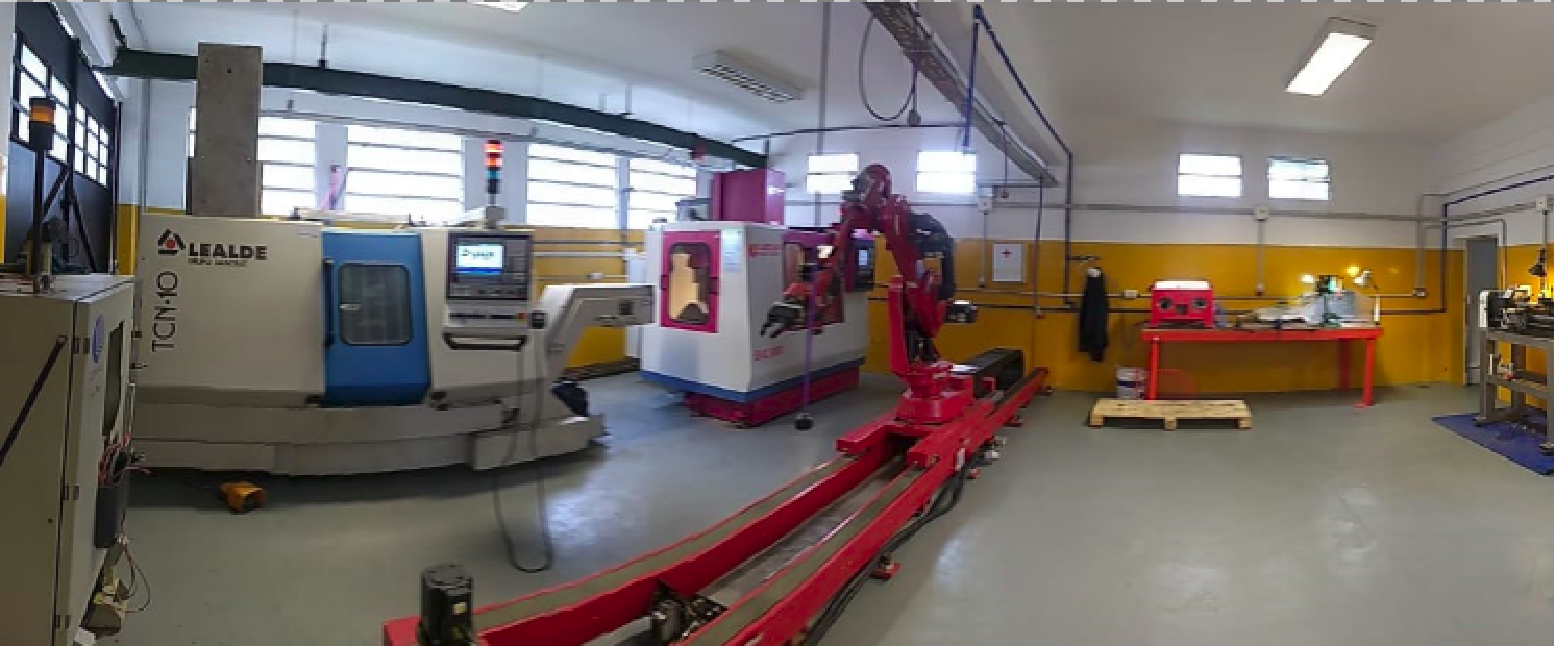
\includegraphics[width=0.85\textwidth]{./Figures/taller_v3.pdf}
\caption{Centro Tecnológico FUNINTEC.}
\label{fig:taller}
\end{figure}

La empresa también cuenta con un laboratorio de electrónica con equipos para diseño y prototipado electrónico.

%----------------------------------------------------------------------------------------
%	SECTION 2
%----------------------------------------------------------------------------------------
\section{Técnicas de dip coating}

En los laboratorios de investigación aplicados en nanotecnologías existen diferentes equipos para la fabricación de películas delgadas o \textit{thin films} que consisten en capas de material de espesores variables, que comúnmente van desde las centenas de nanómetros hasta las decenas de micrómetros y se depositan sobre diferentes superficies.


\textit{Dip coating} es una técnica que se emplea tanto en áreas de I+D (investigación y desarrollo) en la industria, como en la investigación científica en el campo de las nanociencias, se basa en la inmersión y extracción  controlada de un sustrato en una solución química bajo estudio. En la figura \ref{fig:inmersion} se observa una ejecución completa del movimiento desarrollado por el equipo.


\begin{figure}[htpb]
\centering 
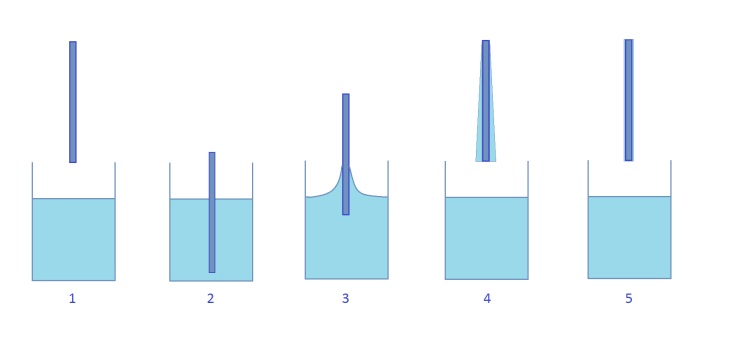
\includegraphics[width=0.85\textwidth]{./Figures/dip-coating.png}
\caption{Proceso completo desarrollado por el equipo \protect\footnotemark.}
\label{fig:inmersion}
\end{figure}
\footnotetext{Imagen tomada de \citep{web_nadetech}}

\begin{enumerate}
\item La muestra desciende a velocidad controlada.
\item La muestra queda sumergida un tiempo establecido por el usuario.	
\item La muestra asciende a velocidad controlada, este es el punto más crítico del experimento, en donde el material queda adherido a la muestra, se estudiará en el capítulo \ref{Chapter3} dos modelos matemáticos que explican este fenómeno y se dará una noción mas detallada de las velocidades que caracterizan el proceso.
\item Se extrae toda la muestra.
\item El usuario puede tener interés o no, en volver a repetir el proceso un tiempo después.
\end{enumerate} 
 
La principal característica del equipo es darle al usuario la posibilidad de controlar la velocidad y aceleración de inmersión de la muestra, el tiempo de espera que la muestra queda sumergida y la extracción, teniendo la posibilidad de repetir el ciclo según se desee.

Como ejemplo de los resultados que se obtienen aplicando está técnica podemos observar en la figura \ref{fig:muestras} films de dioxido de titanio \ce{TiO2}. En la imagen A el film se preparó sobre un wafer de silicio y en la imagen B sobre un portaobjeto de vidrio.


\begin{figure}[!htpb]
     \centering
     \begin{subfigure}[b]{0.4\textwidth}
         \centering
         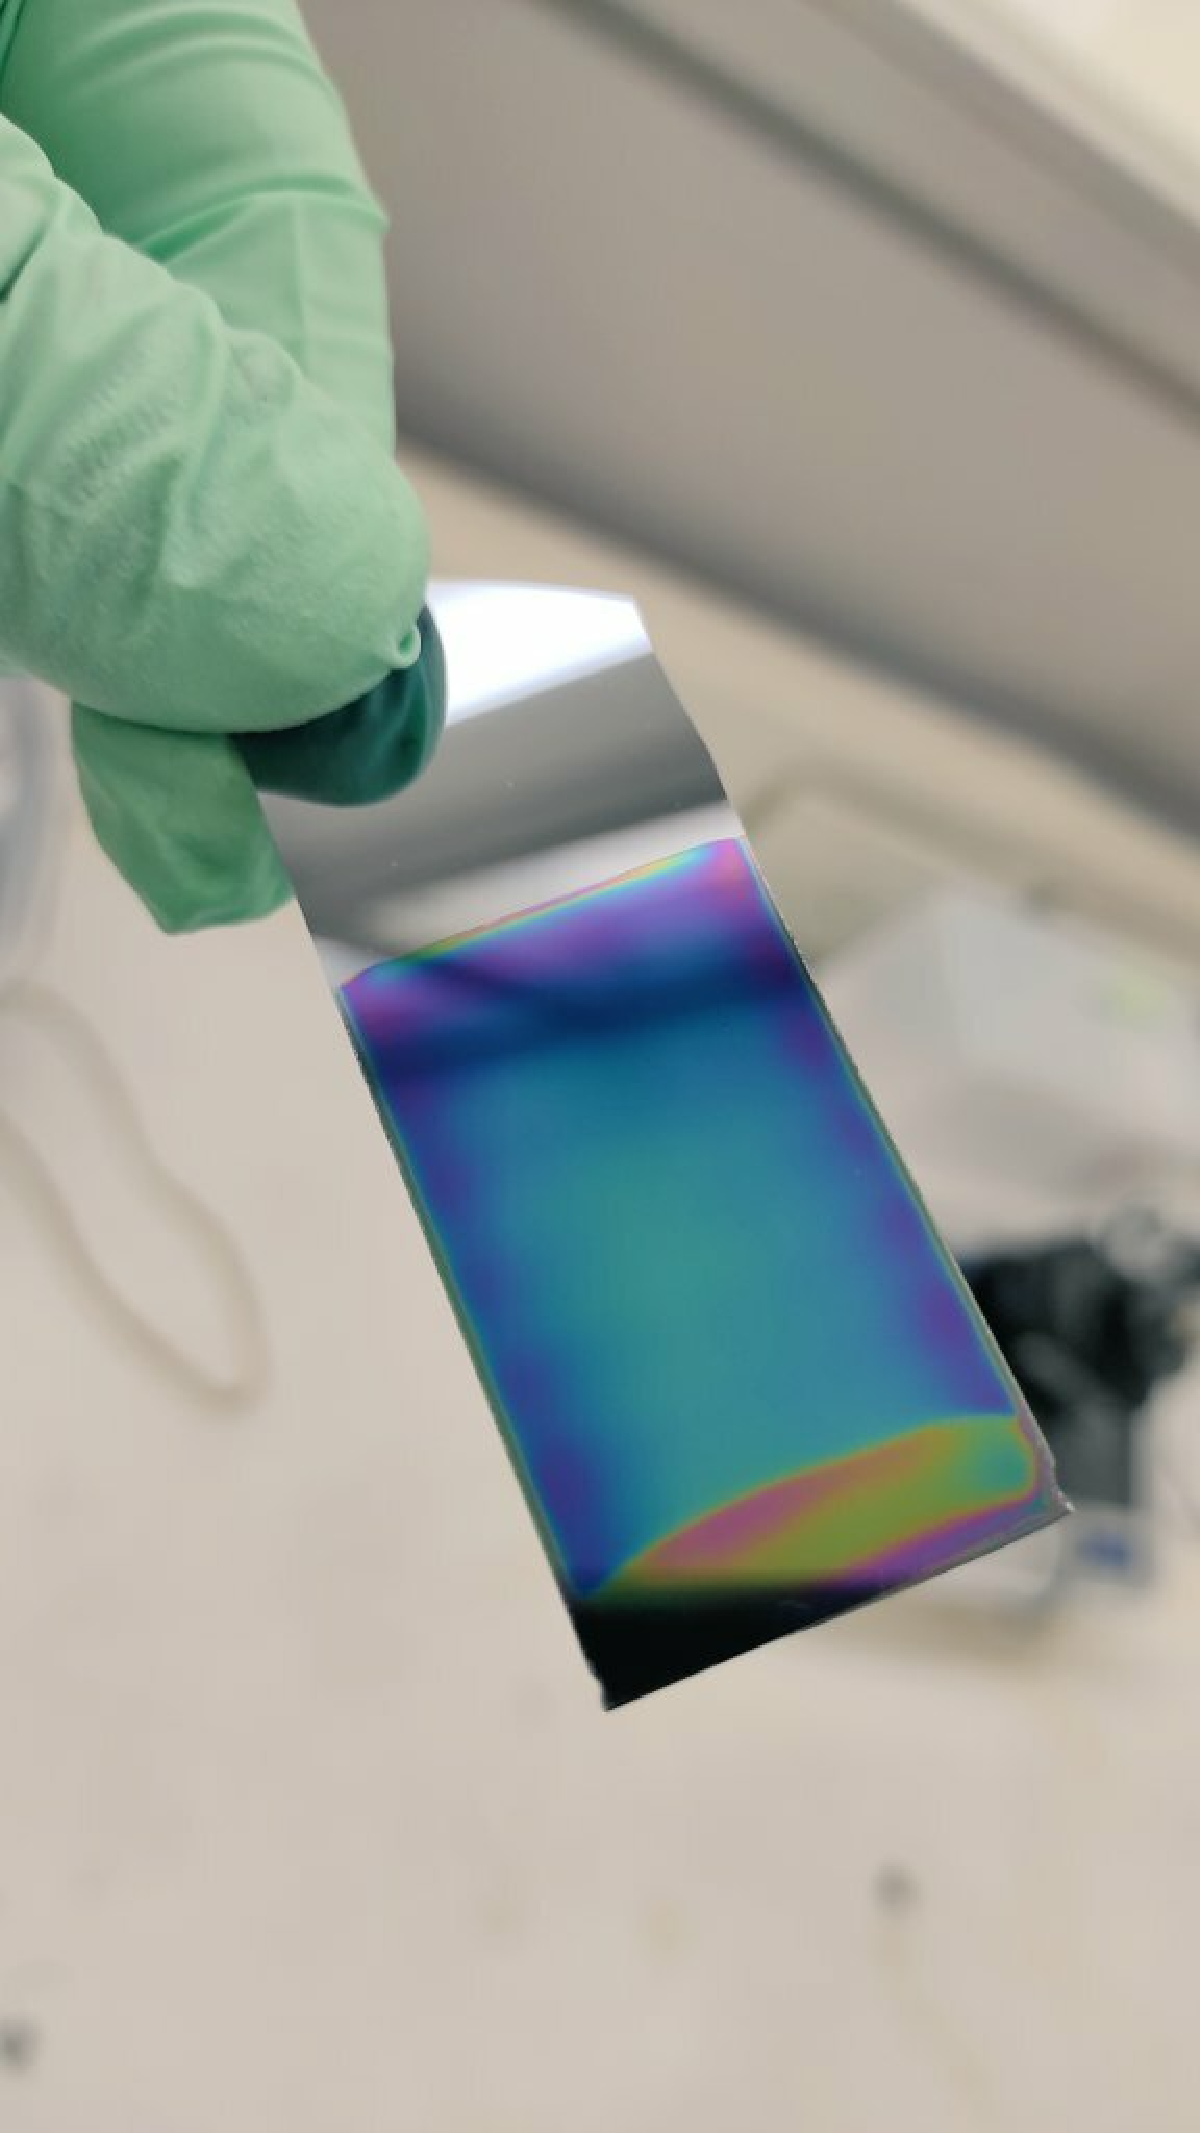
\includegraphics[width=.5\textwidth]{./Figures/muestra_1.pdf}
         \caption{Film sobre wafer de silicio.}
         \label{fig:muestra_1}
     \end{subfigure}
     \hfill
     \begin{subfigure}[b]{0.4\textwidth}
         \centering
         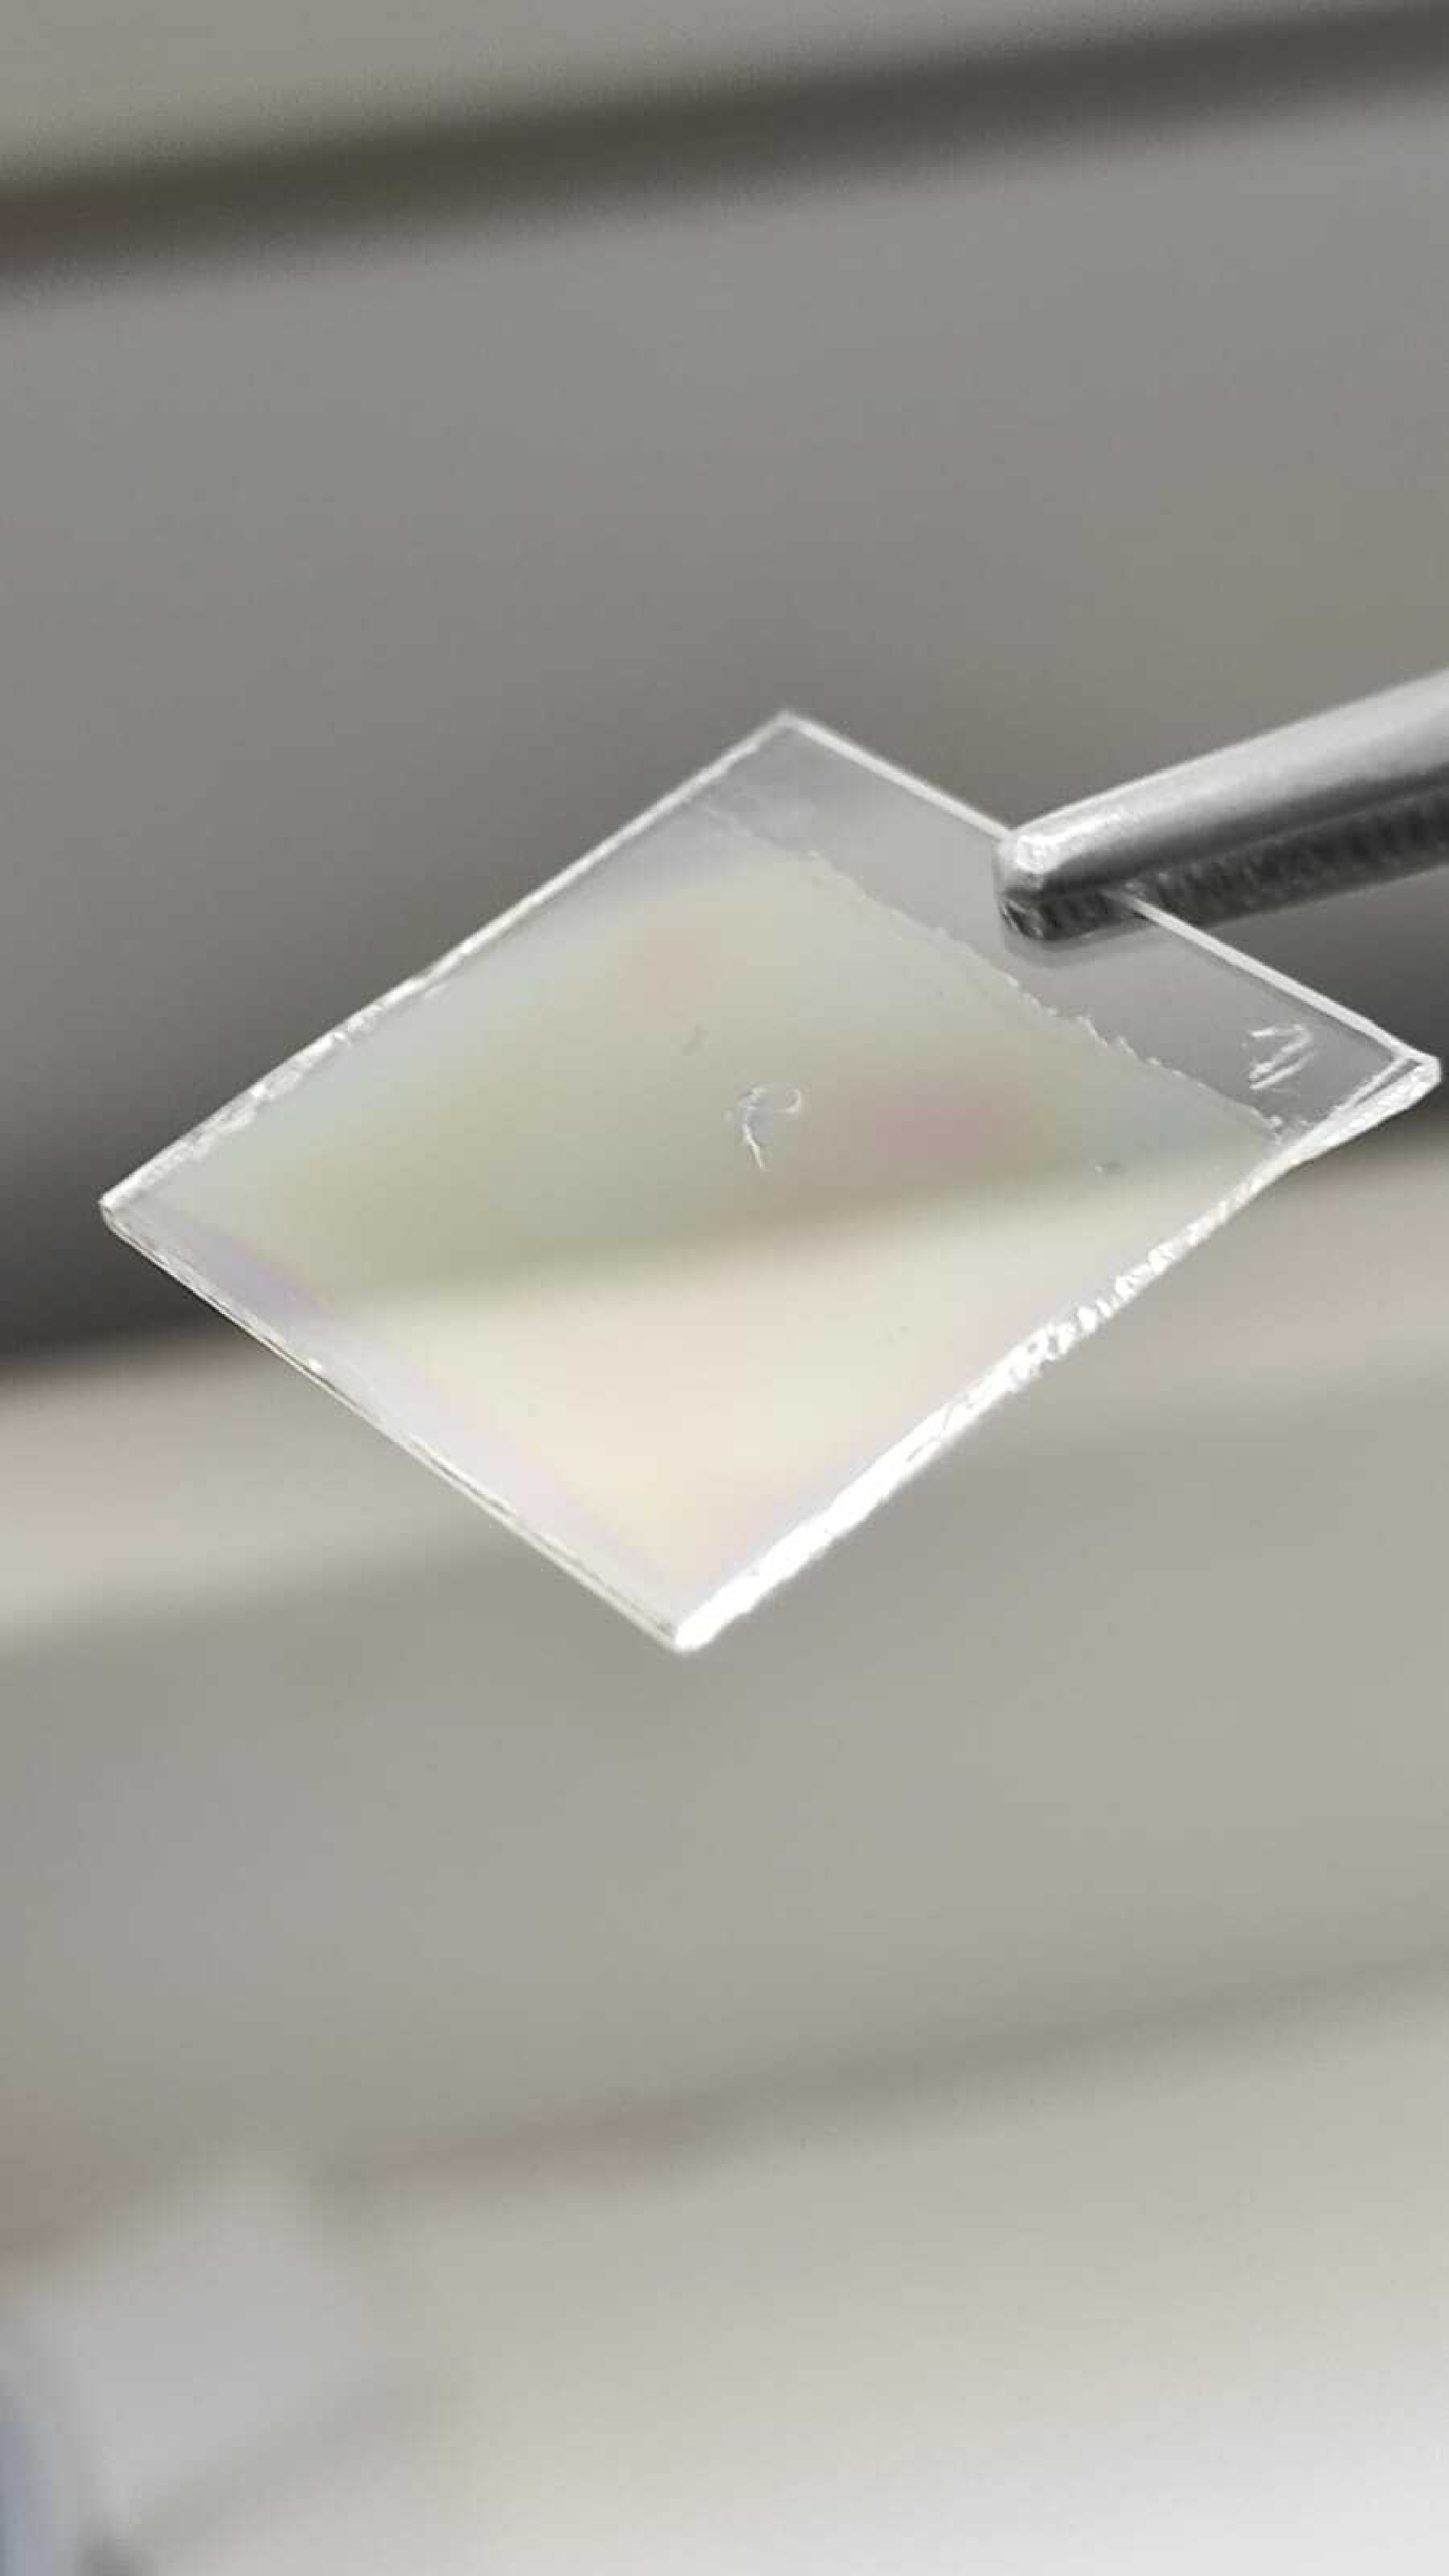
\includegraphics[width=.5\textwidth]{./Figures/muestra_2.pdf}
         \caption{Film sobre portaobjeto.}
         \label{fig:muestra_"}
     \end{subfigure}
     \hfill
        \caption{Films de dioxido de titanio \ce{TiO2} \protect\footnotemark.}
        \label{fig:muestras}
\end{figure}

\footnotetext{Imagen tomada en los laboratorios del Instituto de Nanosistemas de la UNSAM.}


Cabe destacar que los espesores logrados en este experimento fueron entre \SI{180}{nm} y \SI{200}{nm} y la velocidad de inmersión y extracción de los sustratos de \SI{180}{mm/min}.

Luego de un proceso dip coating, dependiendo del tipo de muestra que se genere, es necesario realizar tratamientos térmicos para finalizar el proceso, que se realizan con otro tipo de equipos y por lo tanto no serán parte de esta memoria.
 
\label{sec:dip coating}

%----------------------------------------------------------------------------------------
%	SECTION 3
%----------------------------------------------------------------------------------------
\section{Dip coaters en el mercado}
\label{sec:mercado}
Existen diferentes fabricantes a nivel internacional que comercializan este tipo de equipos pero ninguno a nivel local. Se presentan a continuación algunos equipos de diferentes fabricantes. 

Podemos observar en la figura \ref{fig:dip_kibron} el equipo de la empresa Kibron \citep{2_web_kibron}.

\begin{figure}[htbp]
	\centering
	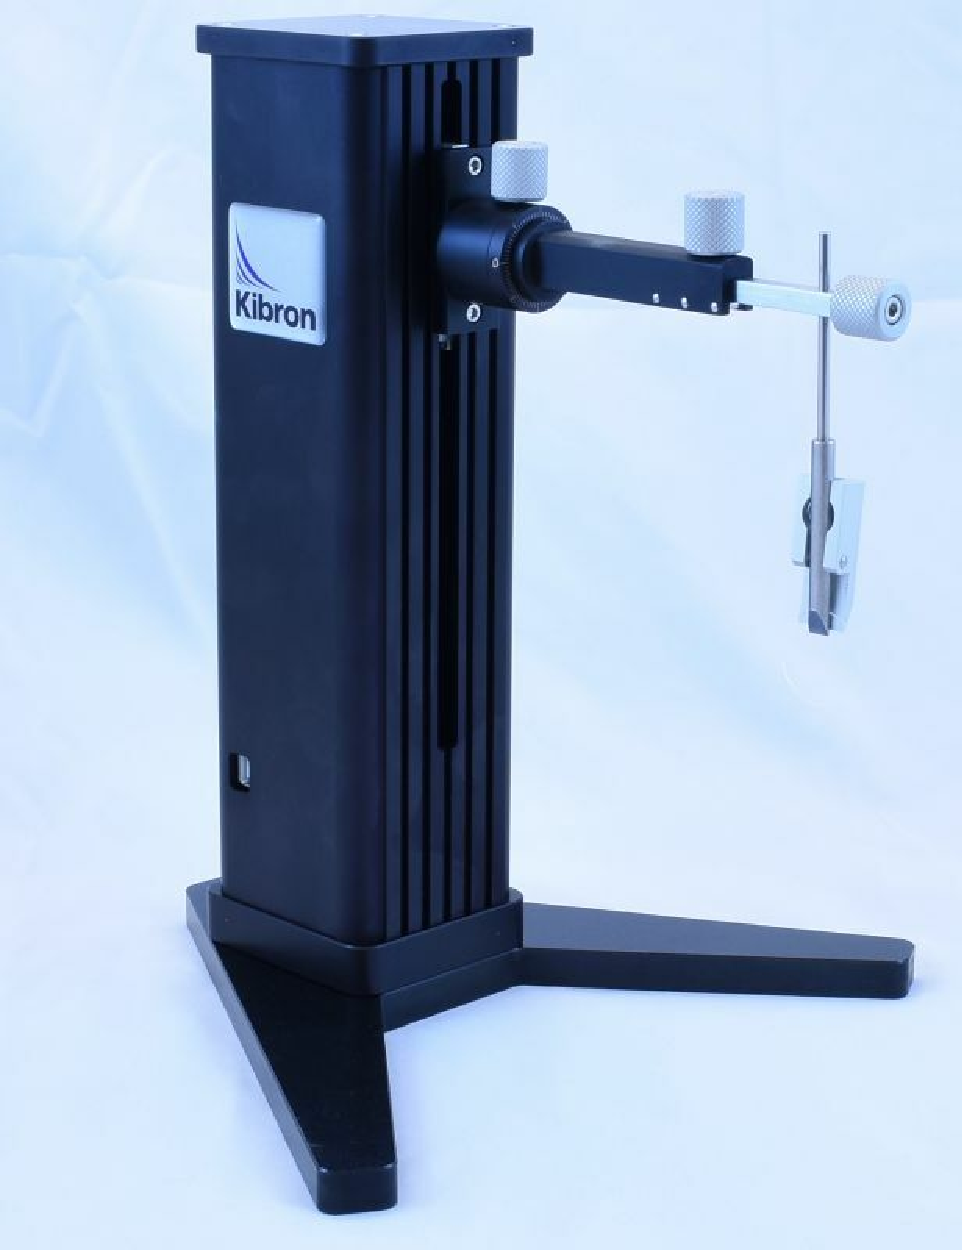
\includegraphics[width=.25\textwidth]{./Figures/kibron.pdf}
	\caption{Equipo de la empresa Kibron.}
	\label{fig:dip_kibron}
\end{figure}

En la figura \ref{fig:equipos_biolin} podemos ver los equipos de la empresa Biolin Scientific  \citep{1_web_biolin}, un equipo simple y otro con mayor funcionalidad. Si bien ambos controlan con exactitud la velocidad de inmersión y extracción, el último agrega una funcionalidad extra, que a través de una rotación en la base da la posibilidad de cambiar de manera automática y secuencial las soluciones donde se realizan las inmersiones. Ambos equipos necesitan estar conectados a una computadora corriendo un software para poder ser accionados.

\begin{figure}[!htpb]
     \centering
     \begin{subfigure}[b]{0.4\textwidth}
         \centering
         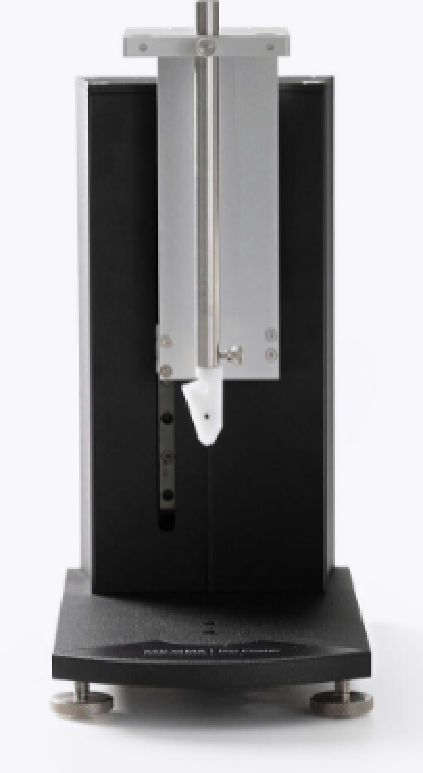
\includegraphics[width=.45\textwidth]{./Figures/dip_biolin.pdf}
         \caption{Equipo simple.}
         \label{fig:dip_biolin}
     \end{subfigure}
     \hfill
     \begin{subfigure}[b]{0.4\textwidth}
         \centering
         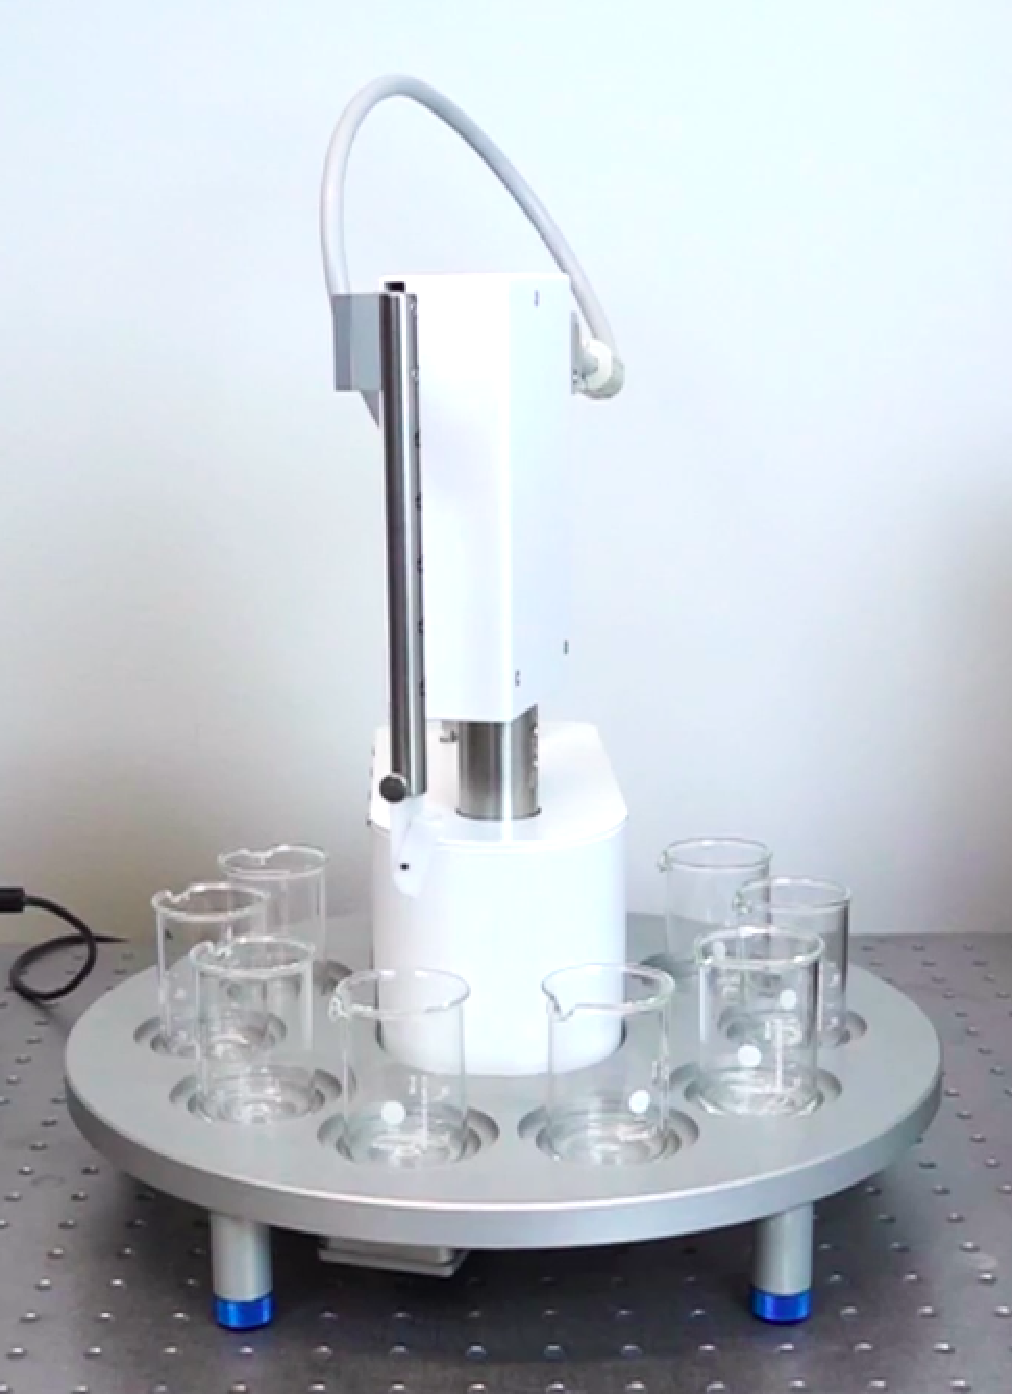
\includegraphics[width=.65\textwidth]{./Figures/dip_biolin_2.pdf}
         \caption{Equipo avanzado.}
         \label{fig:dip_biolin_2}
     \end{subfigure}
     \hfill
        \caption{Equipos de la empresa Biolin Scientific.}
        \label{fig:equipos_biolin}
\end{figure}

Por último presentamos el equipo de la empresa Bungard \citep{6_web_bungard}, que puede observarse en la figura \ref{fig:dip_bungard}.
Este equipo a diferencia de los otros cuenta con un display LCD y botonera, que permite al usuario realizar una configuración a pie de máquina.

\begin{figure}[htbp]
	\centering
	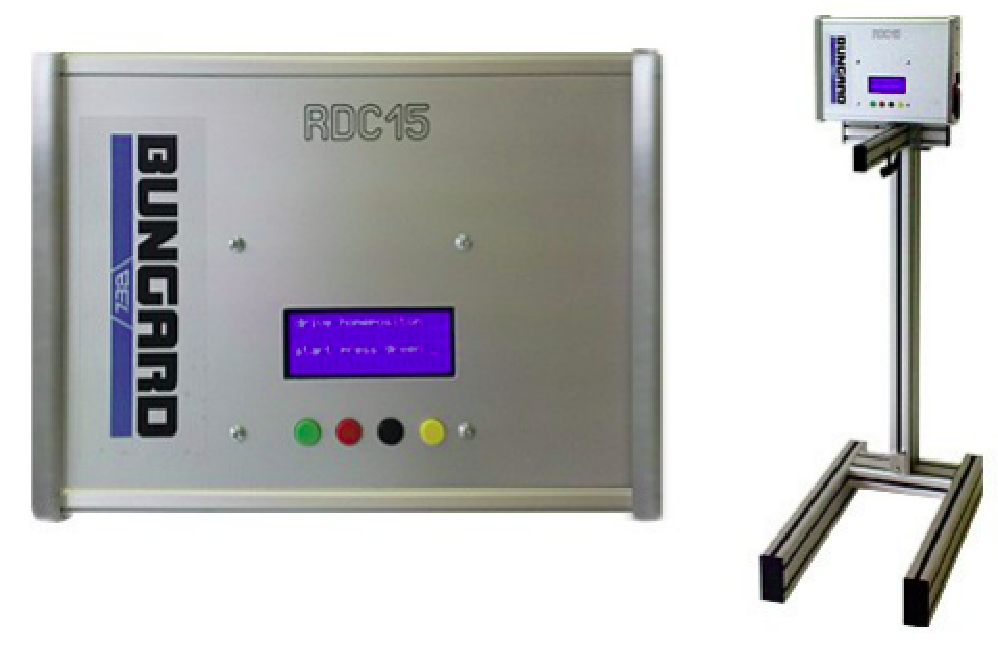
\includegraphics[width=.45\textwidth]{./Figures/6_bungard.pdf}
	\caption{Equipo de la empresa Bungard.}
	\label{fig:dip_bungard}
\end{figure}

A continuación se presenta la tabla \ref{tab:equipos_competencia} en donde se comparan las especificaciones técnicas que los caracterizan.

\begin{table}[h]
	\centering
	\caption[Dip coaters en el mercado]{Especificaciones técnicas de otros equipos.}
	\begin{tabular}{l c c c c}    
		\toprule
		\textbf{Equipo} 	 & \textbf{Recorrido}  & \parbox{2cm} {\textbf{Velocidad (mm/min)}}  & \parbox{2cm}{\textbf{Aceleración (m/min2)}}  & \textbf{Interface} \\
		\midrule
		Bio Single Vessel M	& 300 mm 	& 1    - 1000   & no & PC 							\\		
		Bio Multiplie Vessel		& 70  mm	& 0.1  - 108 	& no & PC					\\
		Kibron LayerX				& 134 mm	& 0.06 - 300	& no & PC					\\
		Bungard						& 600 mm	& 30 - 10000	& no & Display LCD		\\
		Ossila \citep{4_web_ossila}					& 100 mm	& 0.6  - 3000	& no & PC		\\
		Holmarc	\citep{5_web_holmarc}					& 100 mm	& 1.08 - 540	& no & PC		\\
		\bottomrule
		\hline
	\end{tabular}
	\label{tab:equipos_competencia}
\end{table}

Podemos entonces extraer algunas conclusiones, ninguno de los equipos permite al usuario tener control sobre la aceleración en los movimientos de inmersión y extracción de muestra, la mayoría  de los equipos depende de una comunicación USB-SERIAL con una computadora para poder ser ejecutados, ninguna de las empresas adhiere a los principios del software y hardware libre.  

%----------------------------------------------------------------------------------------
%	SECTION 4
%----------------------------------------------------------------------------------------

\section{Objetivos y alcance}

\subsection{Objetivos}

El objetivo de este trabajo fue diseñar y fabricar el primer equipo comercial de la empresa TECSCI, con la perspectiva a futuro de ampliar la gama ofrecida de equipos de laboratorio para la investigación científica.

También es parte de los objetivos fundamentales que el equipo desarrollado incorpore mejoras respecto a sus competidores. Se planteará en los siguientes capítulos un estudio sobre el control de movimientos elegido y se presentará un sistema moderno de configuración de equipo. 

\subsection{Alcance}

El presente trabajo incluye la presentación de un equipo comercial dip coater. 


Abarcó los siguientes puntos:

\begin{itemize}
\item Driver de motor provisto por el fabricante TRINAMIC \citep{3_web_trinamic}.
\item Diseño de hardware con software de diseño KICAD \citep{web_kicad}.
\item Fabricación de placa electrónica y montaje de componentes.
\item Diseño y fabricación de partes mecánicas a través del mecanizado de aluminio.
\item Incorporación de pantalla táctil para configuración y uso del equipo.
\end{itemize}



El trabajo no incluyó:

\begin{itemize}
\item Desarrollo de hardware con fuente de alimentación incorporada.
\item Programación de la interfaz gráfica con el software de diseño provisto por
el fabricante de la pantalla.
\item Control del entorno con registro de humedad, temperatura y  cámara de humedad.
\end{itemize}



% Chapter Template

\chapter{Introducción específica} % Main chapter title

\label{Chapter2} % Change X to a consecutive number; for referencing this chapter elsewhere, use \ref{ChapterX}

%----------------------------------------------------------------------------------------
%	SECTION 1
%----------------------------------------------------------------------------------------
En el presente capítulo se introducen los módulos principales del equipo dip coater fabricado.   

\section{Estudio preliminar}

Para entender la relación entre la velocidad de extracción y el espesor de material depositado se tuvo en consideración la siguiente publicación \textit{(Preparation of Sol-Gel Films by Dip-Coating)} \cite{paper_galo}, que describe la técnica dip coating como un proceso dinámico, complejo y difícil de modelar, debido a los gradientes de concentración y viscosidad generados por evaporación de la solución. 


La publicación se basa entonces en un estudio semi-experimental sobre varias soluciones químicas para predecir el espesor final de la película. Tiene en cuenta dos modelos matemáticos, un modelo de capilaridad asociado a extracciones en velocidades bajas y otro modelo de evaporación asociado a velocidades altas respecto al rango de estudio. 

Se observa en la figura \ref{fig:paper_galo} la variación de los espesores fabricados respecto a las velocidades utilizadas, también se puede observar la relación entre los diferentes modelos aplicados. 

\begin{figure}[!h]
\centering 
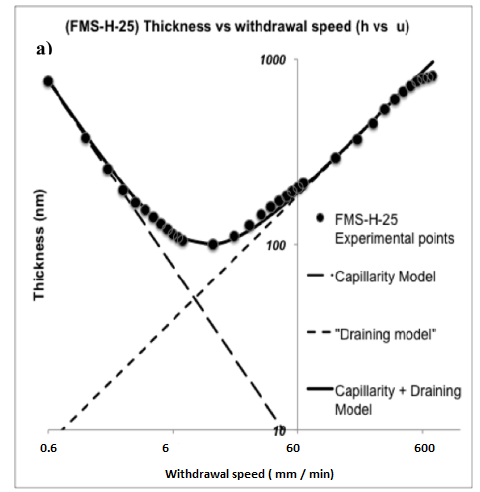
\includegraphics[width=0.52\textwidth]{./Figures/paper_galo.png}
\caption{Espesor vs velocidad \protect\footnotemark.}
\label{fig:paper_galo}
\end{figure}

\footnotetext{Imagen tomada de \cite{paper_galo}.}


Los resultados del experimento concluyen en que existe linealidad en la relación de espesor respecto a la velocidad de extracción entre \SI{60}{\milli\meter\per\minute} y \SI{600}{\milli\meter\per\minute} . También demuestra que en dicho rango de velocidades el fenómeno se explica por el modelo de evaporación.

Se desprende de este análisis la importancia de los siguientes requerimientos funcionales definidos por el cliente: 

\begin{itemize}
\item El sistema debe contar con un rango de velocidades de desplazamiento de muestra entre [1- 1000 \si{\milli\meter\per\minute}]. 
\item El sistema debe contar con un rango de aceleraciones de desplazamiento de muestra entre [1000 - 15000 \si{\meter\per\square\minute}].
		
\end{itemize}
	
Cabe destacar que todos los experimentos en la publicación fueron realizados a velocidad constante. De las reuniones con el cliente y del interés de trabajar en la frontera de la ciencia surgió la necesitad de poder darle al usuario la posibilidad de realizar experimentos a velocidad y aceleración controlada. Esto último es una cualidad que diferencia a este equipo respecto de todos los equipos comerciales analizados en la sección \ref{sec:mercado}.

 
%Sin embargo, es una técnica muy difundida porque es simple y proporciona una excelente reproducibilidad. 
%El problema con este modelo es que la mayoría de las soluciones utilizadas son fluidos no-newtonianos, %es decir en donde el solvente de la solución se va evaparonado en simultáneo con la extracción de la %muestra induciendo una modificación en la densidad, tensión superficial y viscosidad del fluido. 
%Existen modelos matemáticos basados en la mecánica newtoniana que no tienen en cuenta la evaporación de %las soluciones y requieren varias suposiciones y simplificaciones. En estos modelos llegar a la %predicción del espesor depende de la densidad, la tensión superficial y la viscosidad del fluido. 
%La importancia de estos resultados es que el rango de velocidades quedá incluido dentro de los %requerimientos de nuestro equipo. 


\section{Circuitos integrados Trinamic}
\label{sec:Circuitos integrados Trinamic}

%De los siguientes requerimientos funcionales acordados con el cliente:
De reuniones con el cliente en donde se remarcó la importancia de trabajar con un control preciso de motor y en base a experiencias de uso de equipos con tecnologías similares, surge el interés de trabajar con un fabricante de driver específico. Se definen entonces los siguientes requerimientos:
			
\begin{itemize}
\item El equipo deberá contar con un motor paso a paso Nema 17 \citep{web_nema17}  para realizar los movimientos.
\item Se utilizará un driver de motor de la marca Trinamic Motion Control.
\end{itemize}

Trinamic \citep{3_web_trinamic} se especializa en la fabricación de CI (Circuitos Integrados) para el control de diferentes tipos de motores, su tecnología se basa en convertir señales digitales en movimientos controlados. Tiene una amplia experiencia en la industria del control de motores y sus CI son utilizados en una gran variedad de productos. Recientemente fue adquirida por la compañía Analog Devices \citep{web_analogdevices}.

Cabe destacar que los integrados fabricados por la empresa Trinamic se utilizan en diversas aplicaciones en donde la precisión es importante, como por ejemplo: impresión 3D, automatización industrial, robótica y equipos de laboratorio médico entre otras.
Cuenta con una amplia gama de productos que se diferencian principalmente según el tipo de motor que se quiera accionar. Luego de estudiar las diferentes alternativas ofrecidas se eligió trabajar con el driver TMC5130 \citep{3_web_trinamic_producto}.
  
Todos los CI requieren una configuración inicial de parámetros que depende del tipo de motor y de la carga asociada al mismo. Para encontrarla la empresa ofrece el software TMCL-IDE y diferentes placas de desarrollo para trabajar sobre los diferentes drivers. La placa de desarrollo que corresponde al integrado seleccionado es la \textit{TMC5130-Eval Evaluation Board} \citep{3_web_trinamic_placa}.

El TMCL-IDE se ejecuta sobre una placa de desarrollo general compatible con diferentes kits de evaluación. En la figura \ref{fig:tmc5130_placa} se observa a izquierda la placa Startrampe  que se conecta entre la computadora y la placa de evaluación \textit{TMC5130-Eval} que se observa a derecha. 

\begin{figure}[htpb]
\centering 
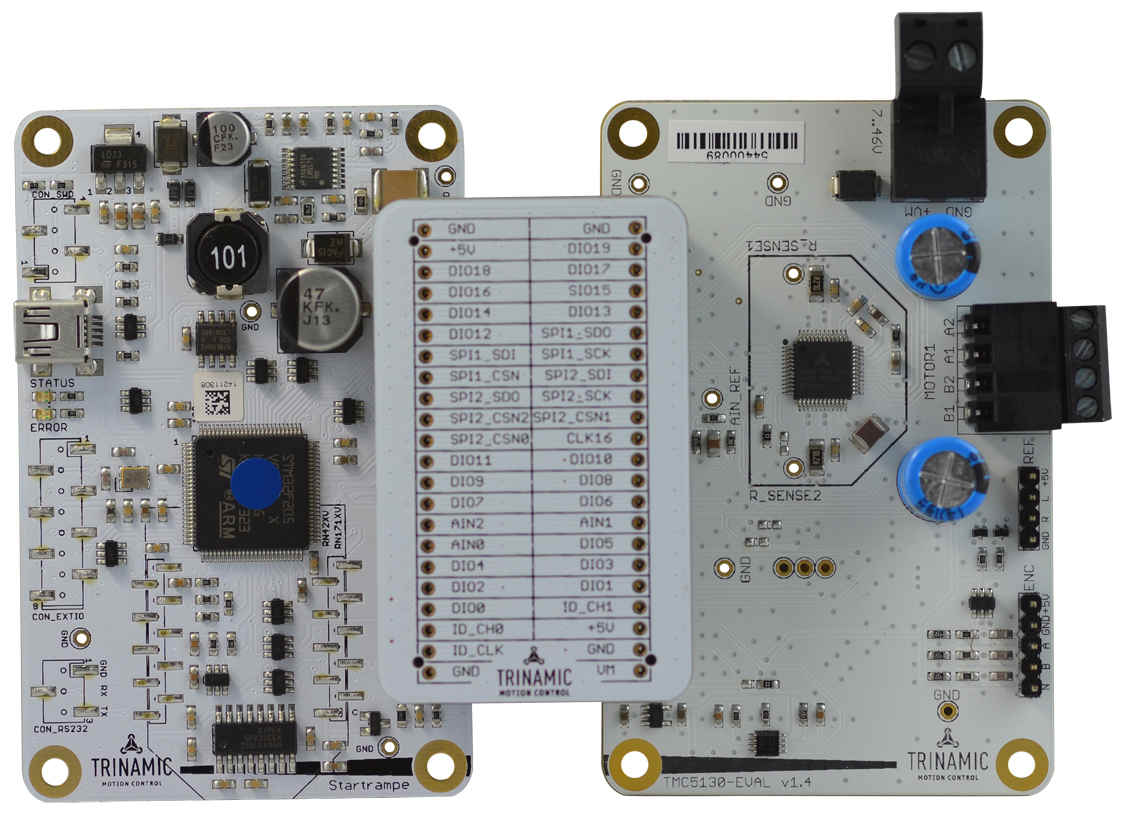
\includegraphics[width=0.7\textwidth]{./Figures/tmc5130_placa_v2.jpg}
\caption{Placa de desarrollo Startrampe + placa de evaluación TMC5130 \protect\footnotemark.}
\label{fig:tmc5130_placa}
\end{figure}

\footnotetext{Imagen tomada de \cite{3_web_trinamic}.}


  
\subsection{Driver TMC5130}
\label{subsection:Driver TMC5130}
El driver TMC5130 permite operar motores bipolares de dos fases comúnmente conocidos como motores paso a paso. El CI incorpora una etapa de potencia con tecnología \textit{MOSFET (Metal Oxide Semiconductor Field Effect Transistor)}  que permite manejar corrientes de hasta dos amperios por fase. Se observa en la figura \ref{fig:tmc5130_diagrama} el diagrama en bloque del CI.

\begin{figure}[htpb]
\centering 
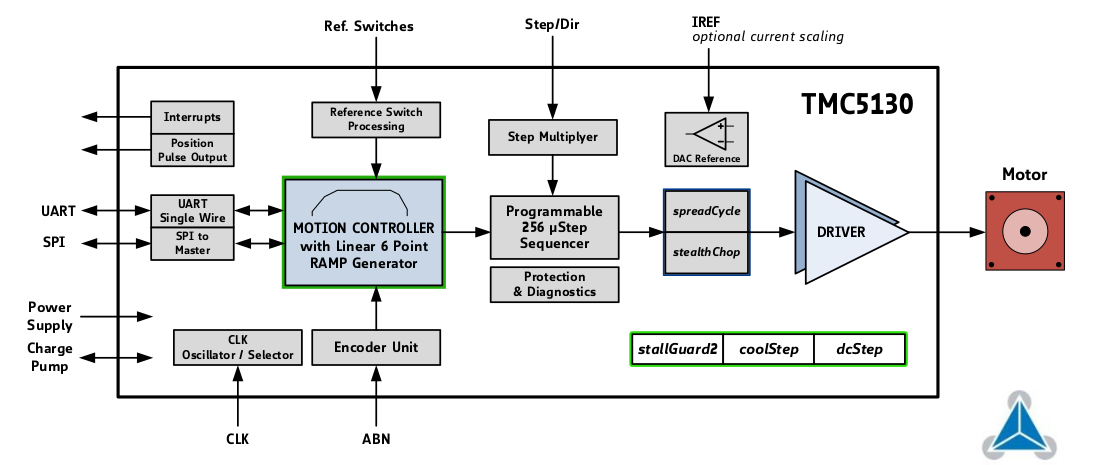
\includegraphics[width=1.1\textwidth]{./Figures/tmc5130_diagrama.png}
\caption{Diagrama en bloques TMC5130 \protect\footnotemark.}
\label{fig:tmc5130_diagrama}
\end{figure}
%\footnotetext{Imagen tomada de \cite{3_web_trinamic}.}

La comunicación con el CI se puede establecer a través del protocolo serie o \textit{SPI (Serial Peripheral Interface)}, para el desarrollo de este trabajo se utilizó el protocolo de comunicación SPI.

Los pasos que definen a este tipo de motores están relacionados con las fases y con la cantidad de dientes que tienen en su rotor y estator. Un paso es el movimiento mínimo que el motor puede hacer. Un motor paso a paso, como su nombre lo indica, realiza movimientos a través de pasos sucesivos. Por ejemplo, es común contar con algún motor en donde la especificación indica que el paso es de \ang{1.8}, esto significa que por cada vuelta de motor \ang{360}, el mismo realizará 200 pasos.

Una funcionalidad que incorpora este CI es incrementar la cantidad de pasos, el fabricante los denomina micropasos. El driver puede generar hasta un máximo de 256 micropasos por cada paso del motor. Siguiendo con el ejemplo recién presentado, para un motor de paso \ang{1.8} se tendrán en total 51200 micropasos, como se observa en la ecuación \ref{eq:micro_pasos}.

\begin{equation}
	\label{eq:micro_pasos}
		(360/1.8) * 256 = 51200 \textup{ micropasos por revolución}
\end{equation}


Una característica importante a destacar es la posibilidad de programar la cantidad de pasos que da el motor. El CI cuenta con el registro XACTUAL que contiene la cantidad de pasos absolutos desde una referencia inicial. También cuenta con el registro XTARGET que contiene una posición objetivo, cuando se escribe este registro el CI se acciona hasta lograr que XACTUAL = XTARGET.

%El motor estará acoplado a un eje lineal que generará movimientos ascendentes y descendentes. Sobre este eje lineal se acoplará un carro de aluminio que tendrá una pinza que sostendrá las muestras. 

Otra funcionalidad que se utilizó fue \textit{stallguard2}, una función que mide la fuerza contraelectromotriz generada en las bobinas del motor por cambios de carga en el eje. En la figura \ref{fig:tmc5130_stallGuard2} se observa que el valor del registro stallguard2 se decrementa linealmente a medida que la carga aumenta. Cuando se aplica una fuerza contraría al movimiento programado o el recorrido del carro llega a un límite mecánico, la fuerza contraelectromotriz aumenta. 

\begin{figure}[h]
\centering 
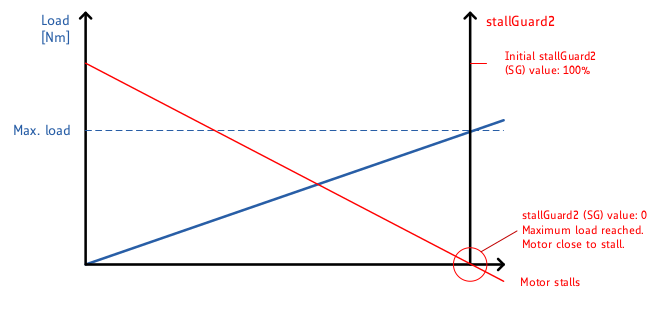
\includegraphics[width=0.8\textwidth]{./Figures/tmc5130_stallguard2.png}
\caption{Función stallguard2.\protect\footnotemark.}
\label{fig:tmc5130_stallGuard2}
\end{figure}
\footnotetext{Imagen tomada de \cite{3_web_trinamic}.}


En el capítulo \ref{Chapter3} se estudiará el valor del registro  stallguard2 configurado. Cada vez que el equipo se enciende se realiza un movimiento hacia un extremo del recorrido para buscar el cero de máquina. Se utiliza esta medida para encontrar un límite mecánico del sistema y realizar  un posicionamiento inicial. El uso de esta funcionalidad evita la incorporación de finales de carrera electromecánicos.   


También se utilizó \textit{coolstep}, una función que a través de mediciones de carga en el eje del motor adapta automáticamente la corriente suministrada hacia las bobinas, aumentando la eficiencia energética como puede observarse en la figura \ref{fig:tmc5130_coolStep}. El efecto final es reducir la energía suministrada según la hoja de datos \citep{3_web_trinamic_producto} hasta un \SI{75}{\percent}. Esto aplica incluso en equipos donde la carga es constante, como es el caso del dip coater, ya que la carga variable representada por un wafer de silicio o un portaobjeto es completamente despreciable.

\begin{figure}[h]
\centering 
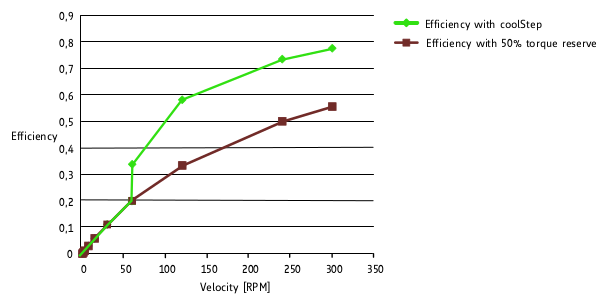
\includegraphics[width=1\textwidth]{./Figures/tmc5130_coolstep.png}
\caption{Función coolstep.\protect\footnotemark.}
\label{fig:tmc5130_coolStep}
\end{figure}
\footnotetext{Imagen tomada de \cite{3_web_trinamic}.}

Por último, se utilizó la función \textit{dcStep}, que es un modo de conmutación automático que ajusta la velocidad del motor en caso de existir sobrecarga en el eje, es decir que si no puede mover la carga acoplada al eje con la velocidad establecida, se ajusta a una velocidad menor para poder seguir en movimiento y no detenerse por completo. 


%el capítulo \ref{Chapter3} se darán detalles de las configuraciones finales del equipo.
El driver TMC5130 cuenta con cincuenta registros que se utilizan para configurar las funcionalidades del CI y controlar el motor. En el capítulo \ref{Chapter3} se darán más detalles de los registros configurados con la ayuda del software TMCL-IDE.  


\section{Interfaz de usuario}
\label{sec:interfaz_pantalla}

Respecto a la interacción entre el usuario y el equipo surgió en reuniones con el cliente la necesidad de contar con una interfaz moderna, que permita a un usuario dentro de un laboratorio configurar al equipo a pie de máquina. Dando lugar al siguiente requerimiento:
\begin{itemize}
\item La configuración de la máquina debe poder realizarse a través de una pantalla táctil.	
\end{itemize} 

Se decidió trabajar con pantallas del tipo \textit{HMI (Human Machine Interface)}. Las mismas se encargan exclusivamente del procesamiento gráfico. En general, cuentan con un software de diseño para la creación de la interfaz gráfica, es decir que permiten crear botones, barras, pantallas y diferentes tipos de objetos para interaccionar con el usuario. Luego se le da funcionalidad a cada uno de estos objetos creados en el software y a través de un protocolo de comunicación se interactúa con el sistema de control, permitiendo finalmente controlar y configurar el equipo. En el caso de este equipo la pantalla se comunica con un microcontrolador, pero  podría  comunicarse con algún otro sistema de control como por ejemplo un  \textit{PLC (Programmable Logic Controller)}.
 

Luego de una investigación de mercado se eligió a la empresa STONE \citep{web_stone}. El fabricante ofrece un catálogo amplio de pantallas que caracteriza según el tipo de aplicación y entorno de trabajo. Ofrece entonces pantallas para usos industriales, civiles o avanzados. Por las dimensiones finales del equipo y el tipo de uso se optó por pantallas avanzadas de 4.3 pulgadas. Se detallan en la tabla \ref{tab:tabla_stone} las características técnicas de dos pantallas de 4.3 pulgadas del fabricante.

\begin{table}[!ht]
	\centering
	\caption[Comparación Stone]{Comparación pantallas táctiles Stone 4.3.}
	\begin{tabular}{l c c }    
		\toprule
		\textbf{}     & \textbf{STWI043WT} & \textbf{STVI043WT} \\
		\midrule
		CPU 			& 	Cortex A8         		& 	CortexM4 			 	\\		
		Refresh Rate    & 	1G Hz         			& 	200 MHz 				\\
		Image format  	& 	png, bmp, jpg, svg, gif     & 	bmp, jpg 				\\
		Resolution		& 	480×272 pixel	        & 	480×272 pixel 			\\
		Flash  			& 	256 MB         			& 	128 MB 					\\
		Color  			& 	262 K	          		& 	65 K 					\\
		PCB 			& 	2.0 mm black, ROHS       & 	1.6 mm green 			\\
		Touch Type		& 	Resistive    			& 	Resistive				\\
		Interface 		& 	RS232/RS422/RS485/TTL   & 	RS232/RS485/TTL			\\
		\bottomrule
		\hline
	\end{tabular}
	\label{tab:tabla_stone}
\end{table}


El modelo elegido fue el STWI043WT, que pertenece a la nueva línea productos, tiene mayor capacidad de procesamiento, cuenta con un software nuevo de configuración con mayores funcionalidades respecto al utilizado por el otro modelo y la diferencia de precios no supera el \SI{15}{\percent}.  

La comunicación de la pantalla STWI043WT con el microcontrolador se estableció a través del protocolo serie.


%El modelo elegido como se observa en la figura \ref{fig:stone}
%\begin{figure}[htpb]
%\centering 
%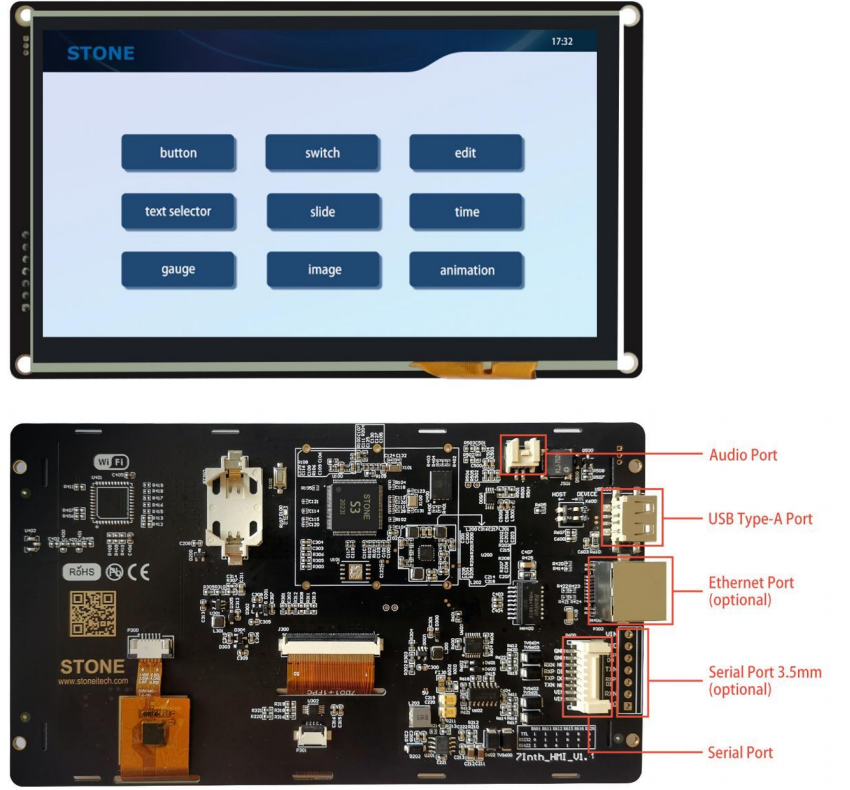
\includegraphics[width=0.5\textwidth]{./Figures/stone.png}
%\caption{Display táctil Stone.}
%\label{fig:stone}
%\end{figure}

\section{Estructura mecánica}
\label{sec:estructura_mecanica}

Se presentan a continuación los siguientes requerimientos asociados a las partes mecánicas del equipo: 

\begin{itemize}
\item La estructura principal del equipo debe ser fabricada con perfil de aluminio anodizado natural.
\item El recorrido mecánico de desplazamiento de muestra debe ser como mínimo de [3500 mm].
\item Las piezas especiales del equipo deben ser mecanizadas en aluminio.

\end{itemize}

Se decidió trabajar con el proveedor Perfiles de Aluminio .NET \citep{web_perfiles_net}, que cuenta con diferentes modelos y dimensiones de perfiles necesarios para la fabricación de la estructura.

El equipo cuenta con una guía lineal acoplada al perfil principal. Para la elección de la misma se tuvieron en cuenta las siguientes consideraciones:

\begin{enumerate}
\item El ambiente cambia  según las soluciones químicas utilizadas. Es posible entonces que se trabaje con soluciones corrosivas que afecten la estructura.  
\item El uso de lubricantes en las guías podría afectar la calidad del experimento.
\item Se deben evitar vibraciones en la estructura para no dañar la calidad del \textit{film}.

\end{enumerate}

Se decidió entonces trabajar con la empresa IGUS \citep{web_igus}, que se especializa en la fabricación de polímeros. La misma ofrece guías lineales que se deslizan en lugar de rodar, y por lo tanto no utilizan rodamientos metálicos. Los polímeros están combinados con materiales anticorrosivos y no requieren de la aplicación de lubricante, es decir, que conforman un entorno de trabajo limpio y libre de mantenimiento periódico. Se observa en la figura \ref{fig:equipo_mecánico} cuatro tipos de guías en donde se puede apreciar el polímero auto-lubricado que se ubica entre el eje y el carro.

\begin{figure}[ht]
\centering 
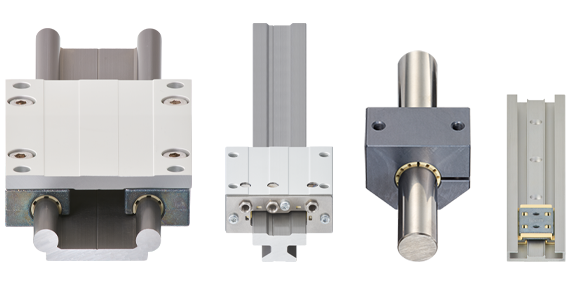
\includegraphics[width=0.7\textwidth]{./Figures/guias.png}
\caption{Guía Lineal IGUS.\protect\footnotemark.}
\label{fig:equipo_mecánico}
\end{figure}
\footnotetext{Imagen tomada de \cite{web_igus}.}


Para el diseño y fabricación de piezas mecanizadas en aluminio se trabajó con el software BOBCAD \citep{web_bobcad} \textit{CAD/CAM (Computer-Aided Design /Computer-Aided Manufacturing )}. Un software  utilizado en la industria manufacturera, que se encuentra constituido por dos módulos fundamentales que permiten abarcar aspectos de diseño y modelado de pieza y luego de fabricación.  

Con la parte CAD se diseña el modelo 3D de la pieza. Con el fin de corregir errores de diseño con mayor velocidad, se realiza una impresión 3D con filamento plástico para probar las dimensiones y la factibilidad técnica de la pieza.
Una vez que el modelo en su versión plástica queda aprobado, se comienza con la configuración del módulo CAM, este módulo se encarga de convertir, a través de diferentes estrategias, al modelo 3D en lenguaje de máquina que el equipo puede interpretar. Se observa en la imagen \ref{fig:fagor} la fresadora CNC de la marca FAGOR \citep{web_fagor} utilizada para la fabricación de las piezas del equipo dip coater. El control de la fresadora interpreta el código G-CODE también conocido como RS-274 \citep{web_gcode} generado por el modulo CAM y lo convierte en movimientos de motores.


\begin{figure}[ht]
\centering 
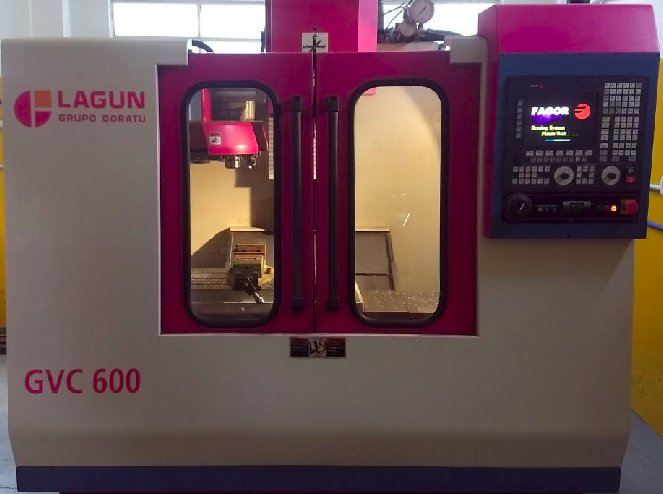
\includegraphics[width=0.7\textwidth]{./Figures/fagor.png}
\caption{Fresadora Fagor GVC 600.\protect\footnotemark.}
\label{fig:fagor}
\end{figure}
\footnotetext{Imagen tomada en el centro tecnológico de FUNINTEC.}
 

\section{Sistema electrónico propuesto}
\label{sec:sistema_propuesto}


Se presentan a continuación los siguientes requerimientos:
\begin{itemize}

\item El sistema debe permitir que el usuario pueda configurar en un programa variables de desplazamiento y tiempos de espera.
\item Un programa previamente configurado debe poder ejecutarse o guardarse en memoria interna.
\item El usuario debe poder guardar al menos 10 programas en la memoria no volátil del sistema.
\item Se debe utilizar control de versionado de cambios durante el desarrollo del firmware.
\item El desarrollo del firmware debe realizarse con capas de abstracción de software de tal manera que permita en un futuro cambiar de microcontrolador sin mayor esfuerzo.
\item El desarrollo se realizará sobre un módulo microcontrolador ESP32.
\item Se deben registrar variables de humedad, presión y temperatura [opcional].
\end{itemize}

De reuniones con el cliente y de la necesidad de trabajar con un equipo que permita a futuro contar con una comunicación Wi-Fi, surgió el requerimiento de trabajar con el módulo ESP32 \citep{web_esp}.
El ESP32 es un módulo del tipo \textit{SoC (System On Chip)}, es decir que además del microcontrolador y sus periféricos internos, agrega periféricos externos para brindar conectividad inalámbrica y almacenamiento extra para datos y programa.
  

Teniendo en cuenta los requerimientos analizados en las secciones previas y los requerimientos analizados en esta sección se propuso, como se observa en la figura \ref{fig:equipo_propuesto}, el siguiente esquema de equipo dip coater.  


\begin{figure}[ht]
\centering 
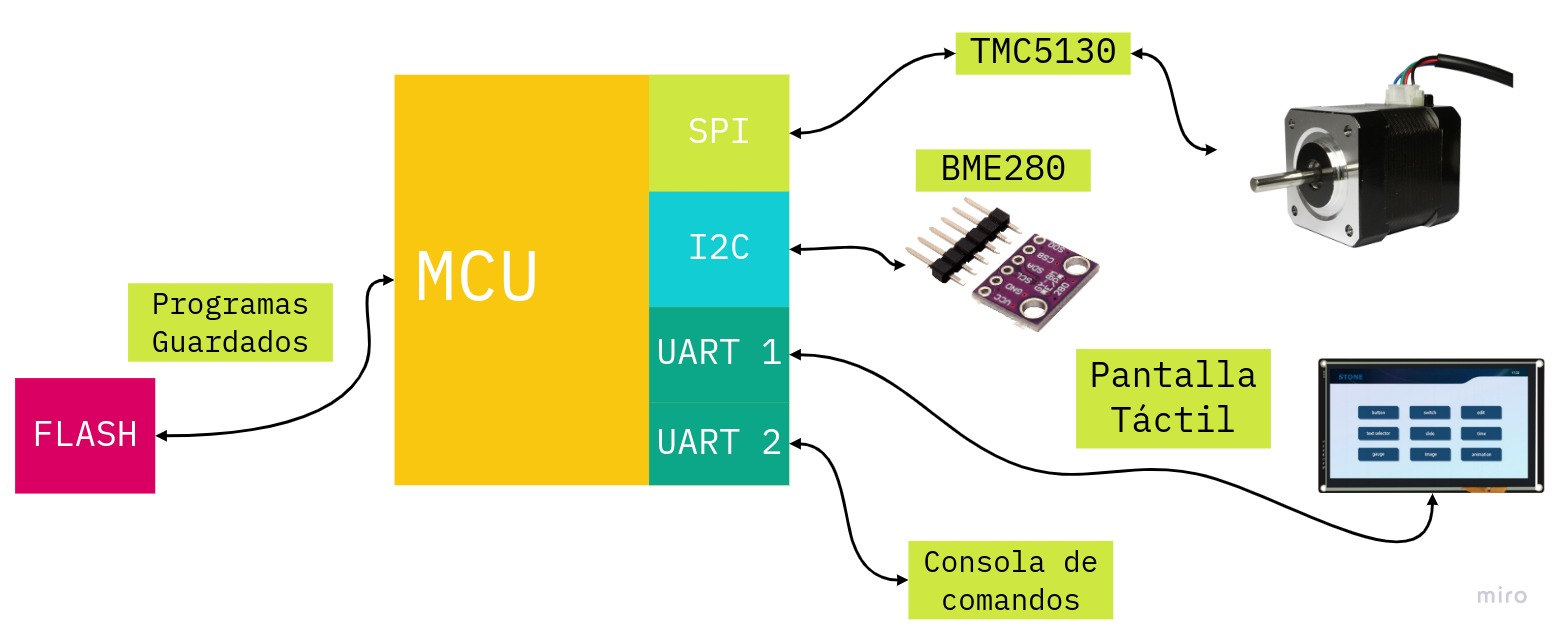
\includegraphics[width=0.9\textwidth]{./Figures/cap2_esquema_propuesto.jpg}
\caption{Esquema de equipo propuesto.}
\label{fig:equipo_propuesto}
\end{figure}

El equipo estará entonces compuesto por el módulo ESP32-WROOM como unidad central de procesamiento. Contará con dos canales de comunicación serie, uno para establecer una consola de comandos que permita comunicar al equipo con una computadora, realizar pruebas de funcionamiento y configuraciones y el otro para comunicarse con la pantalla táctil. También establecerá un protocolo de almacenamiento para guardar los programas que el usuario cree en la memoria FLASH disponible. Finalmente contará con un módulo de comunicación sobre protocolo I2C para obtener datos del sensor de humedad y temperatura BME280.  


\section{Herramientas de desarrollo}

Para la implementación del hardware se utilizó el software libre de diseño de circuitos impresos KICAD \citep{web_kicad}, la elección del mismo se basó en los siguientes puntos:

\begin{itemize}
\item Las capacidades que brinda el software son suficientes para el desarrollo de este hardware.
\item Se valora el apoyo del \textit{CERN:European Organization for Nuclear Research} \citep{1_nota_web_kicad_cern} al proyecto KICAD.
%\item Las últimas versiones presentan mejoras significativas respecto a sus predecesoras.
\end{itemize}


Para la implementación del firmware se trabajó con el \textit{framework} ESP-IDF \citep{web_esp_idf} provisto por el fabricante del microcontrolador. Dicho entorno se ejecuta sobre FreeRTOS, que es un sistema operativo de tiempo real utilizado en dispositivos embebidos que permite un desarrollo de software bajo un esquema multi-tareas.

Se trabajó con el entorno de programación ECLIPSE IDE, la elección se basó en los siguientes puntos:
\begin{itemize}
\item El fabricante del microcontrolador ESPRESSIF ofrece \textit{plugings} para incorporar al entorno y facilitar el desarrollo. 
\item Existe documentación para la configuración del \textit{framework ESP-IDF} \citep{web_esp_idf_eclipse} sobre el entorno.
\end{itemize}
 
% Chapter Template

\chapter{Diseño e Implementación} % Main chapter title

\label{Chapter3} % Change X to a consecutive number; for referencing this chapter elsewhere, use \ref{ChapterX}
En el siguiente capítulo se presenta el diseño y la implementación de las tres partes fundamentales del equipo. Se abarcan aspectos de diseño de hardware, desarrollo de firmware y diseño y fabricación mecánica.
%----------------------------------------------------------------------------------------
%	SECTION 1
%----------------------------------------------------------------------------------------

\definecolor{mygreen}{rgb}{0,0.6,0}
\definecolor{mygray}{rgb}{0.5,0.5,0.5}
\definecolor{mymauve}{rgb}{0.58,0,0.82}
%%%%%%%%%%%%%%%%%%%%%%%%%%%%%%%%%%%%%%%%%%%%%%%%%%%%%%%%%%%%%%%%%%%%%%%%%%%%%
% parámetros para configurar el formato del código en los entornos lstlisting
%%%%%%%%%%%%%%%%%%%%%%%%%%%%%%%%%%%%%%%%%%%%%%%%%%%%%%%%%%%%%%%%%%%%%%%%%%%%%
\lstset{ %
  backgroundcolor=\color{white},   % choose the background color; you must add \usepackage{color} or \usepackage{xcolor}
  basicstyle=\footnotesize,        % the size of the fonts that are used for the code
  breakatwhitespace=false,         % sets if automatic breaks should only happen at whitespace
  breaklines=true,                 % sets automatic line breaking
  captionpos=b,                    % sets the caption-position to bottom
  commentstyle=\color{mygreen},    % comment style
  deletekeywords={...},            % if you want to delete keywords from the given language
  %escapeinside={\%*}{*)},          % if you want to add LaTeX within your code
  %extendedchars=true,              % lets you use non-ASCII characters; for 8-bits encodings only, does not work with UTF-8
  %frame=single,	                % adds a frame around the code
  keepspaces=true,                 % keeps spaces in text, useful for keeping indentation of code (possibly needs columns=flexible)
  keywordstyle=\color{blue},       % keyword style
  language=[ANSI]C,                % the language of the code
  %otherkeywords={*,...},           % if you want to add more keywords to the set
  numbers=left,                    % where to put the line-numbers; possible values are (none, left, right)
  numbersep=5pt,                   % how far the line-numbers are from the code
  numberstyle=\tiny\color{mygray}, % the style that is used for the line-numbers
  rulecolor=\color{black},         % if not set, the frame-color may be changed on line-breaks within not-black text (e.g. comments (green here))
  showspaces=false,                % show spaces everywhere adding particular underscores; it overrides 'showstringspaces'
  showstringspaces=false,          % underline spaces within strings only
  showtabs=false,                  % show tabs within strings adding particular underscores
  stepnumber=1,                    % the step between two line-numbers. If it's 1, each line will be numbered
  stringstyle=\color{mymauve},     % string literal style
  tabsize=2,	                   % sets default tabsize to 2 spaces
  title=\lstname,                  % show the filename of files included with \lstinputlisting; also try caption instead of title
  morecomment=[s]{/*}{*/}
}

\section{Hardware}
\label{section:Hardware}
\subsection{Diseño basado en módulos de hardware libre}
\label{subsection:Diseño basado en módulos de hardware libre}

El diseño de la placa electrónica se baso en el estudio de los siguientes módulos:
\begin{itemize}
\item TMC5130-EVAL \citep{3_web_trinamic_placa}	
\item NodeMCU \citep{web_nodemcu}
\end{itemize}
Se destaca que ambos proyectos adhieren a la filosofía del hardware libre. Por lo tanto se pudieron descargar y estudiar los diagramas esquemáticos de ambas placas. Las primeras pruebas de implementación de hardware se realizaron interconectando ambos módulos como puede observarse en la figura \ref{fig:esp_tmc5130}.

\begin{figure}[!h]
	\centering
	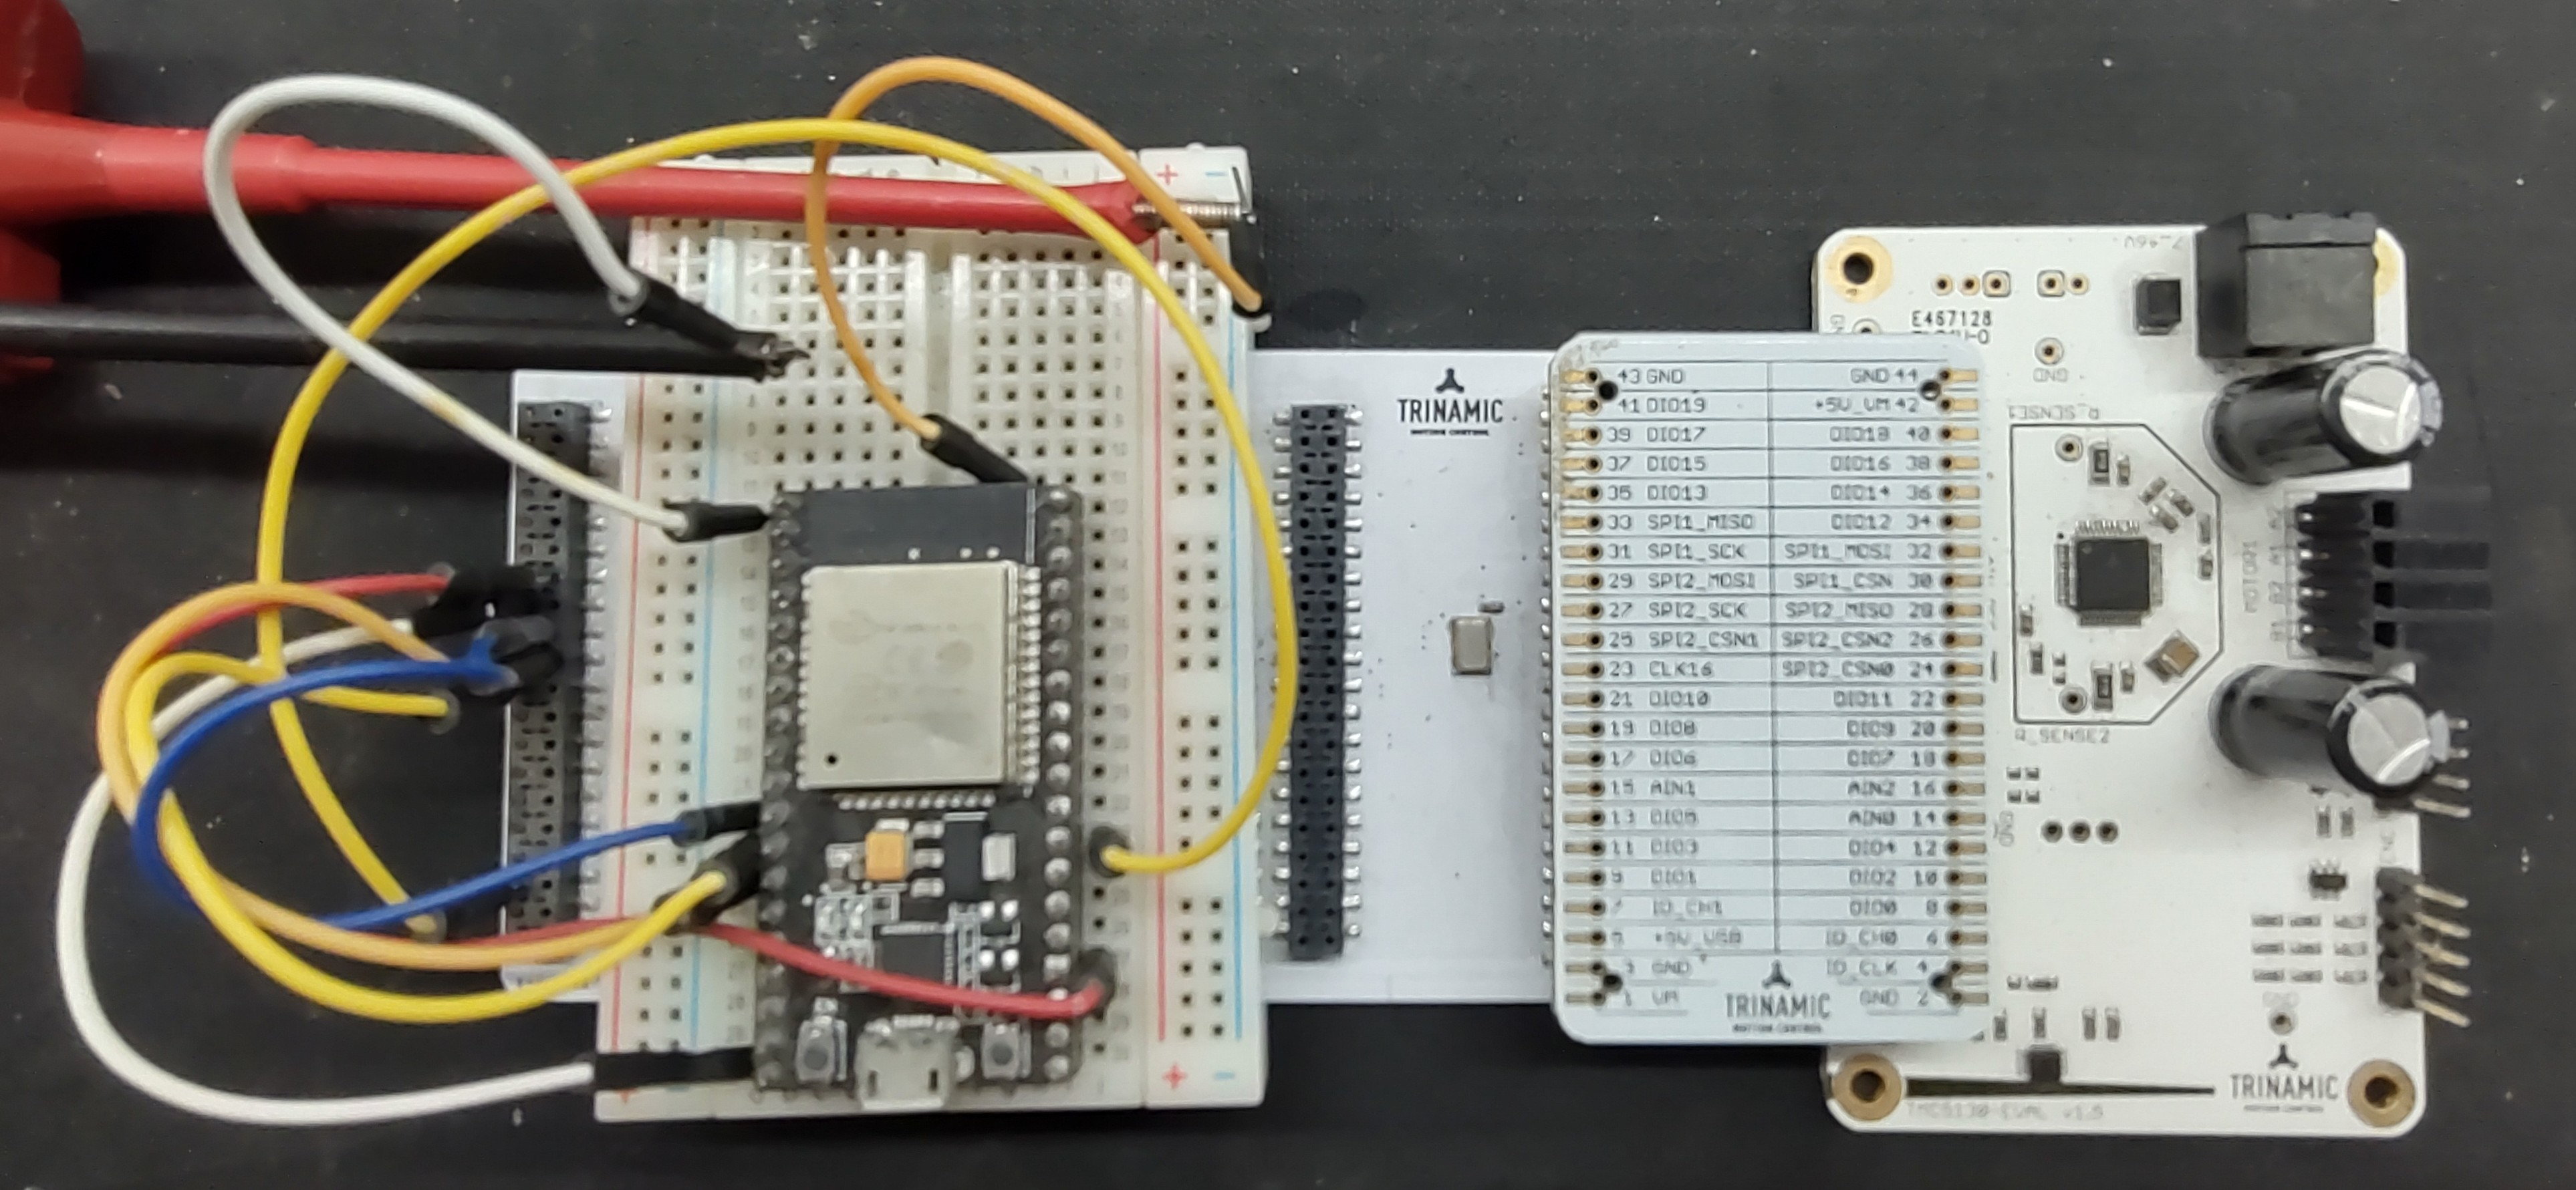
\includegraphics[width=1\textwidth]{./Figures/esp_tmc5130.jpg}
	\caption{Módulo NodeMCU + TMC5130-EVAL.}
	\label{fig:esp_tmc5130}
\end{figure}

\subsection{Etapa de alimentación}

Una etapa importante, que se observa en la figura \ref{fig:kicad_tension}, es la reguladora de tensión que permite alimentar al equipo con tensiones continuas de entre 24 V y 46 V. En el diseño se utilizó el CI LM5161 en modo \textit{step-down buck converter}, una configuración que permite bajar la tensión de entrada según la relación de las resistencias de \textit{feedback}. En este caso se configuró una salida de 5 V la cual tiene una eficiencia energética de 86 \% según su hoja de datos. Luego a través de un regulador de tensión se obtienen 3,3 V que se utilizan para alimentar el microcontrolador.

\begin{figure}[!h]
	\centering
	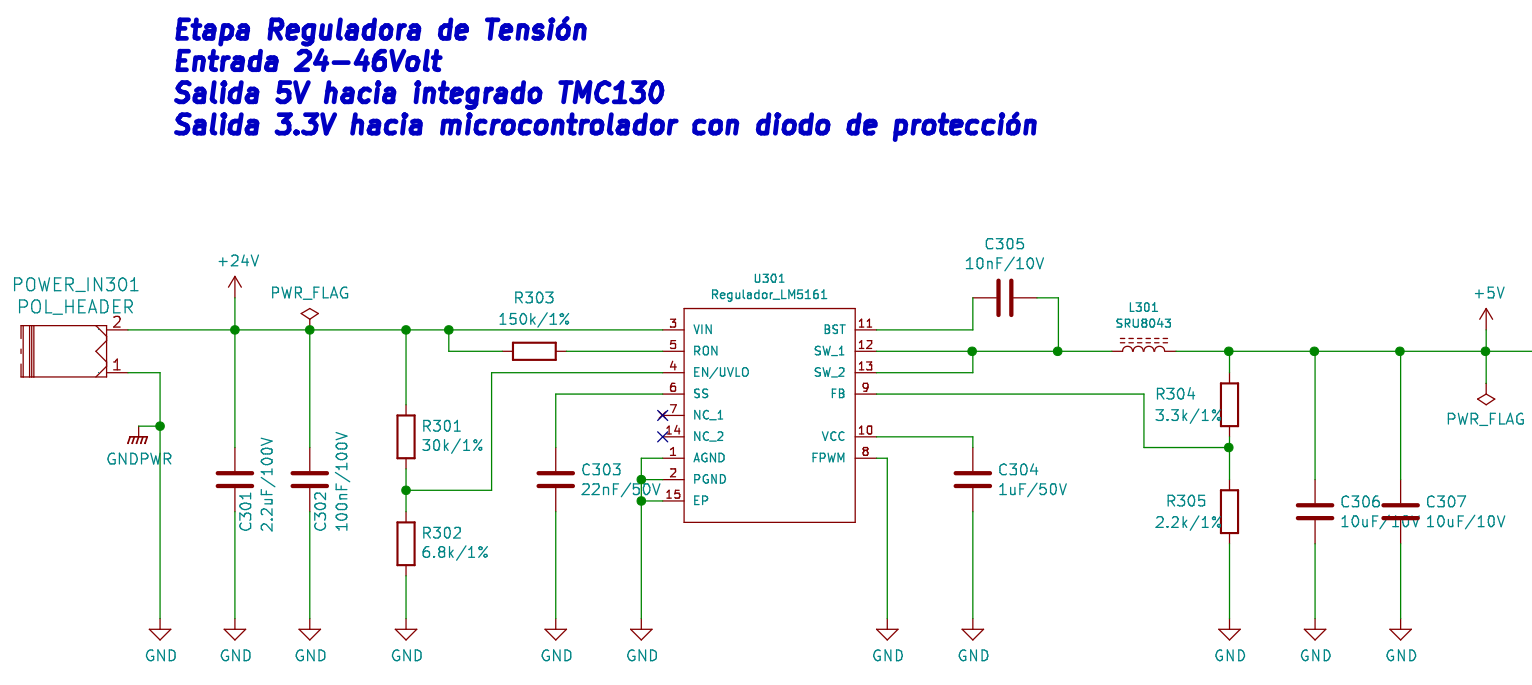
\includegraphics[width=1\textwidth]{./Figures/kicad_tension_v2.png}
	\caption{Módulo de entrada.}
	\label{fig:kicad_tension}
\end{figure}
  
El equipo fue diseñado para ser alimentado con una fuente externa de tensión continua, simplificando así cuestiones regulatorias de certificación que deben cumplir equipos que se alimentan directamente a la red eléctrica.

\subsection{Etapa de comunicación}

El módulo NodeMCU es una placa de desarrollo que contiene el SoC ESP32-WROOM. A partir del estudio de su diseño, se implementó la etapa de conversión SERIAL-USB que puede observase en la figura \ref{fig:kicad_conversor}. 


\begin{figure}[!h]
	\centering
	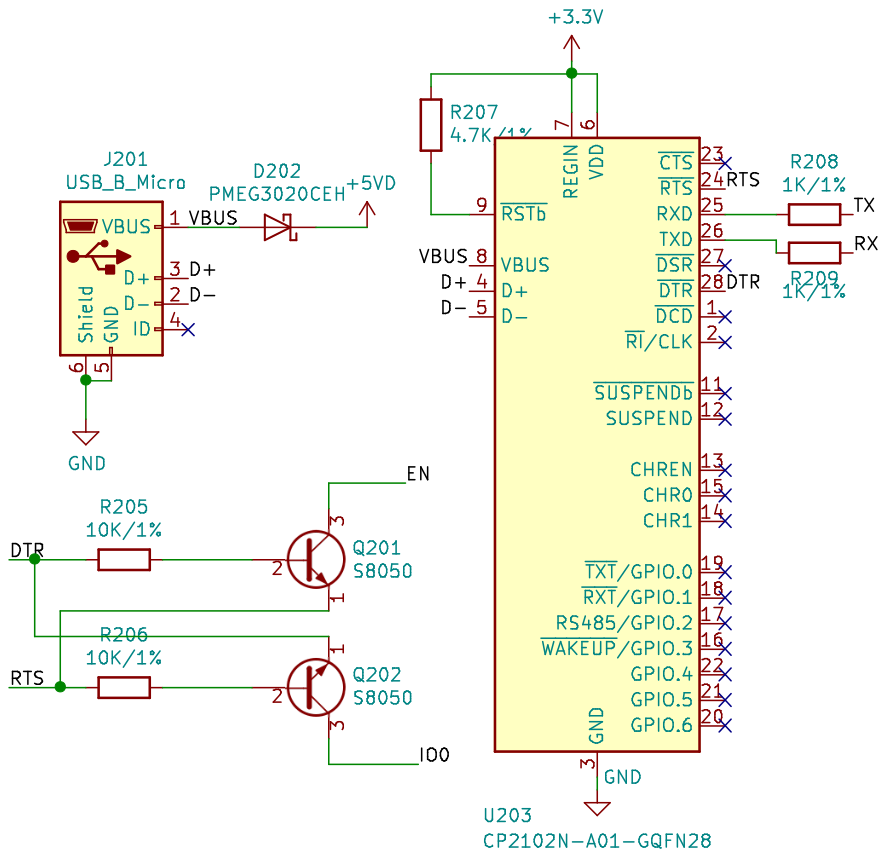
\includegraphics[width=1\textwidth]{./Figures/kicad_conversor_v1.png}
	\caption{Conversor serie-USB.}
	\label{fig:kicad_conversor}
\end{figure}

Mantener esta etapa de entrada en la placa electrónica final habilita la conexión directa del equipo dip coater con un puerto USB de computadora, permitiendo establecer una comunicación constante con el periférico UART y descargar un firmware nuevo sin tener que contar con un programador externo. Se utilizó para esta etapa de conversión el CI CP2102.

Cuando se trabaja con el módulo NodeMCU se debe seguir la siguiente secuencia para descargar el firmware en el microcontrolador:
\begin{enumerate}
\item Apretar el botón \textit{boot} del módulo para poner la terminal IO0 a masa.
\item Sin soltar el boton \textit{boot}, apretar el boton \textit{reset} para inicializar en modo boot.
\item Descargar el firmware con el software de desarrollo. 
\end{enumerate}

La interfaz UART CP2102 consta de señales de transmisión y recepción de datos TX y RX respectivamente, también admite las señales de control RTS/CTS, DSR/DTR y X-On/X-Off. En el diseño se incorporó el uso de las terminales DTR y RTS para generar la secuencia de descarga de manera automática. Sin embargo la misma presentó cierta inestabilidad y no siempre se logró generar la secuencia correctamente, por tal motivo se implementará en la nueva versión de la placa botones para poder forzar dicha secuencia.



\subsection{Driver TMC5130}

El módulo TMC5130-EVAL, como se describió en la sección \ref{sec:Circuitos integrados Trinamic}, contiene al CI TMC5130. Del estudio de esta placa de evaluación se extrajeron las configuraciones necesarias para lograr la correcta utilización del driver. Se tuvieron en cuenta las recomendaciones de diseño establecidas por el fabricante, como por ejemplo la incorporación de un clock externo de 16 MHz, que se puede observar en la figura \ref{fig:kicad_clock} el cual es necesario en aplicaciones de alta precisión. 

\begin{figure}[!h]
	\centering
	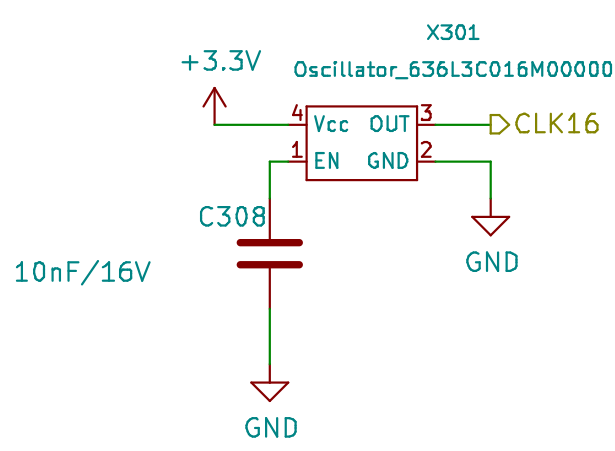
\includegraphics[width=0.5\textwidth]{./Figures/kicad_clock.png}
	\caption{Clock para el CI TMC5130.}
	\label{fig:kicad_clock}
\end{figure}

A continuación, se observa en la figura \ref{fig:kicad_trinamic} las conexiones del driver con el motor paso a paso y el puerto SPI utilizado en la comunicación con el microcontrolador. 
 
\begin{figure}[h]
	\centering
	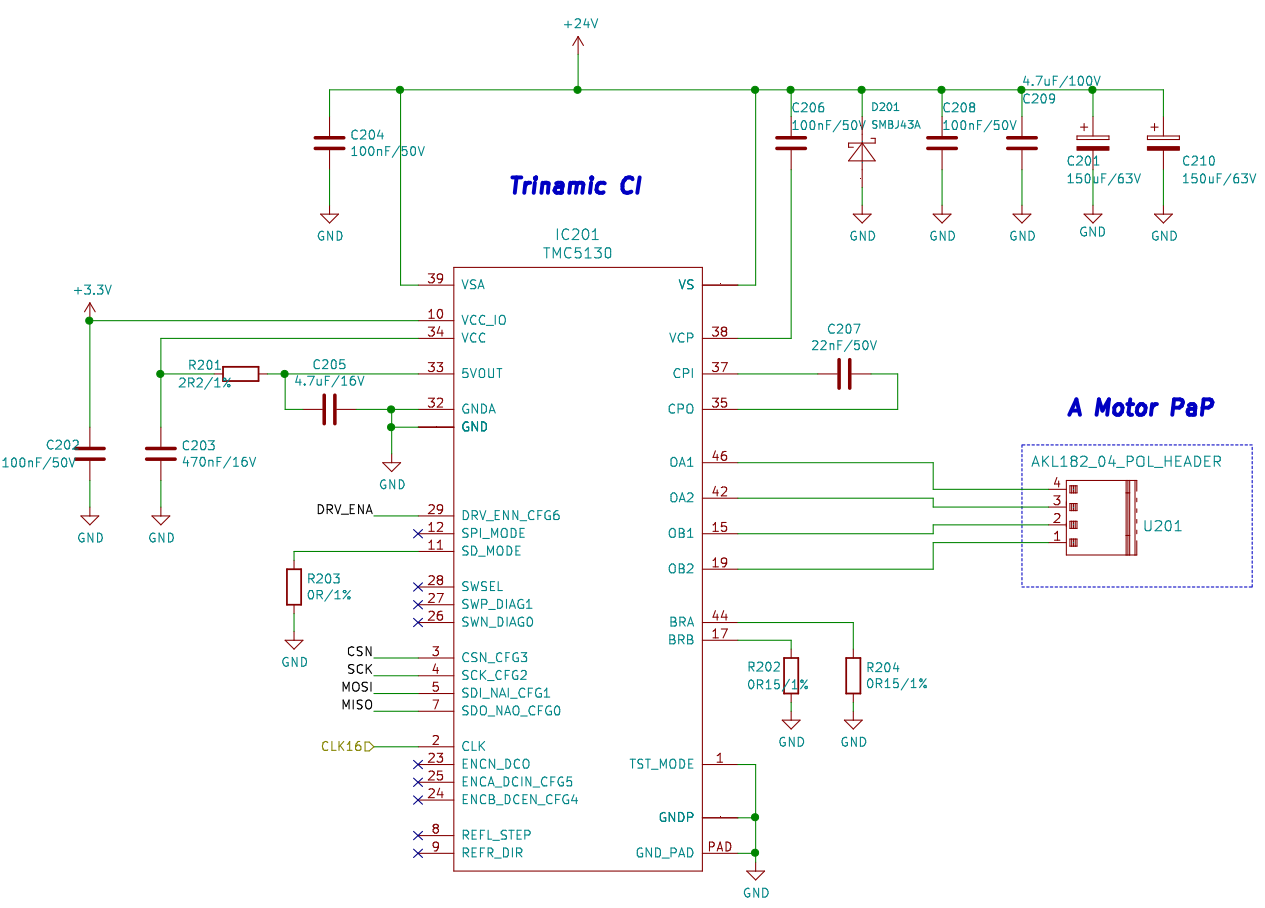
\includegraphics[width=1\textwidth]{./Figures/kicad_trinamic.png}
	\caption{CI TMC5130.}
	\label{fig:kicad_trinamic}
\end{figure} 

%\begin{figure}[h]
%	\centering
%	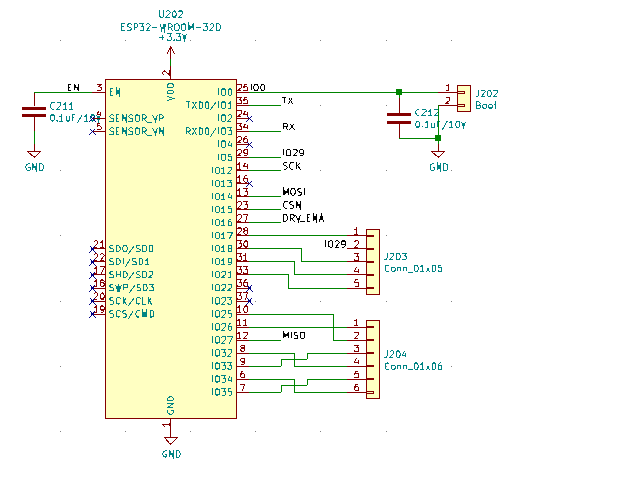
\includegraphics[width=.6\textwidth]{./Figures/kicad_esp.png}
%	\caption{Módulo ESP32.}
%	\label{fig:kicad_esp}
%\end{figure}
  
Finalmente, se observa en la figura \ref{fig:dip_3d_model} el diseño 3D generado por el software KICAD.

Todo el diseño y material asociado se encuentra disponible en el repositorio de la empresa TECSCI \citep{web_hardware_tecsci}. La placa electrónica de este equipo dip coater cuenta con una licencia CERN OHL v.1.2 \citep{web_cern_licence}.


\begin{figure}[!h]
	\centering
	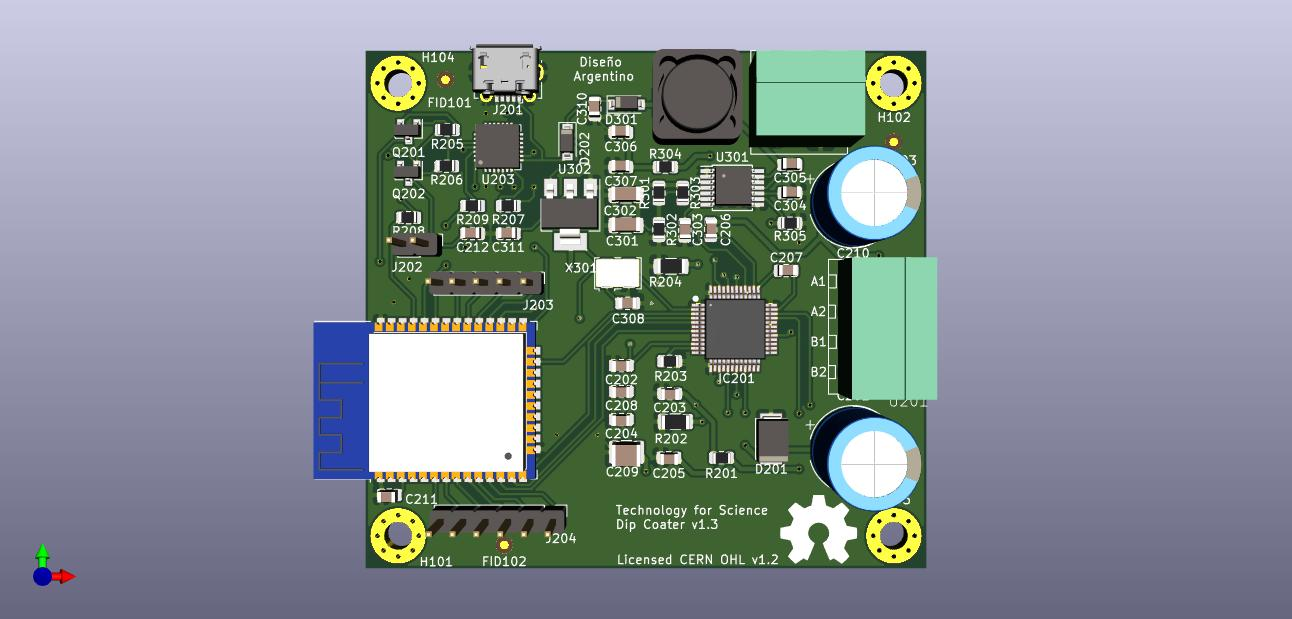
\includegraphics[width=1\textwidth]{./Figures/tecsci_dip.jpg}
	\caption{Modelo 3D Kicad.}
	\label{fig:dip_3d_model}
\end{figure}
         



  
%-----------------------------------
%	SUBSECTION 1
%-----------------------------------
\subsection{Fabricación}
%-----------------------------------
%	SUBSECTION 2
%-----------------------------------
La placa electrónica se fabricó con el proveedor local de circuitos impresos Ernesto Mayer S.A. \citep{web_mayer}. A continuación se presenta la información de diseño de la misma y se describen algunas  restricciones de impuestas por el propio fabricante:

\begin{itemize}

\item Grilla de posicionamiento principal: 0,25 mm.
\item Grilla de ruteo principal: 0,25 mm.
\item Agujeros de montaje: 3,2 mm.
\item Pistas principales: 0,5 mm.
\item Pistas inferiores: 0,25 mm, con límite particular 0,20mm (8 mils).
\item Pistas superiores: 0,8 mm.
\item Vías: 0,8 mm /0,4 mm, con límite particular 0,20mm (8 mils).
\item Margen general: 0,22 mm.
\item Margen particular: 0,2 mm, con límite particular 0,20 mm (8 mils).
\item Fabricación: espesor 1,6mm FR4.  
\item Restricciones generales del fabricante: con límite estándar 0,254 mm (10 mils).

\end{itemize}

Luego de fabricar el PCB, se continuó con el montaje de componentes electrónicos superficiales, que estuvo a cargo de la empresa Asembli S.A. \citep{web_asembli}. Se fabricó un primer lote de cinco placas. En la figura \ref{fig:dip_real_model} se observa la placa con los componentes montados.


\begin{figure}[htbp]
	\centering
	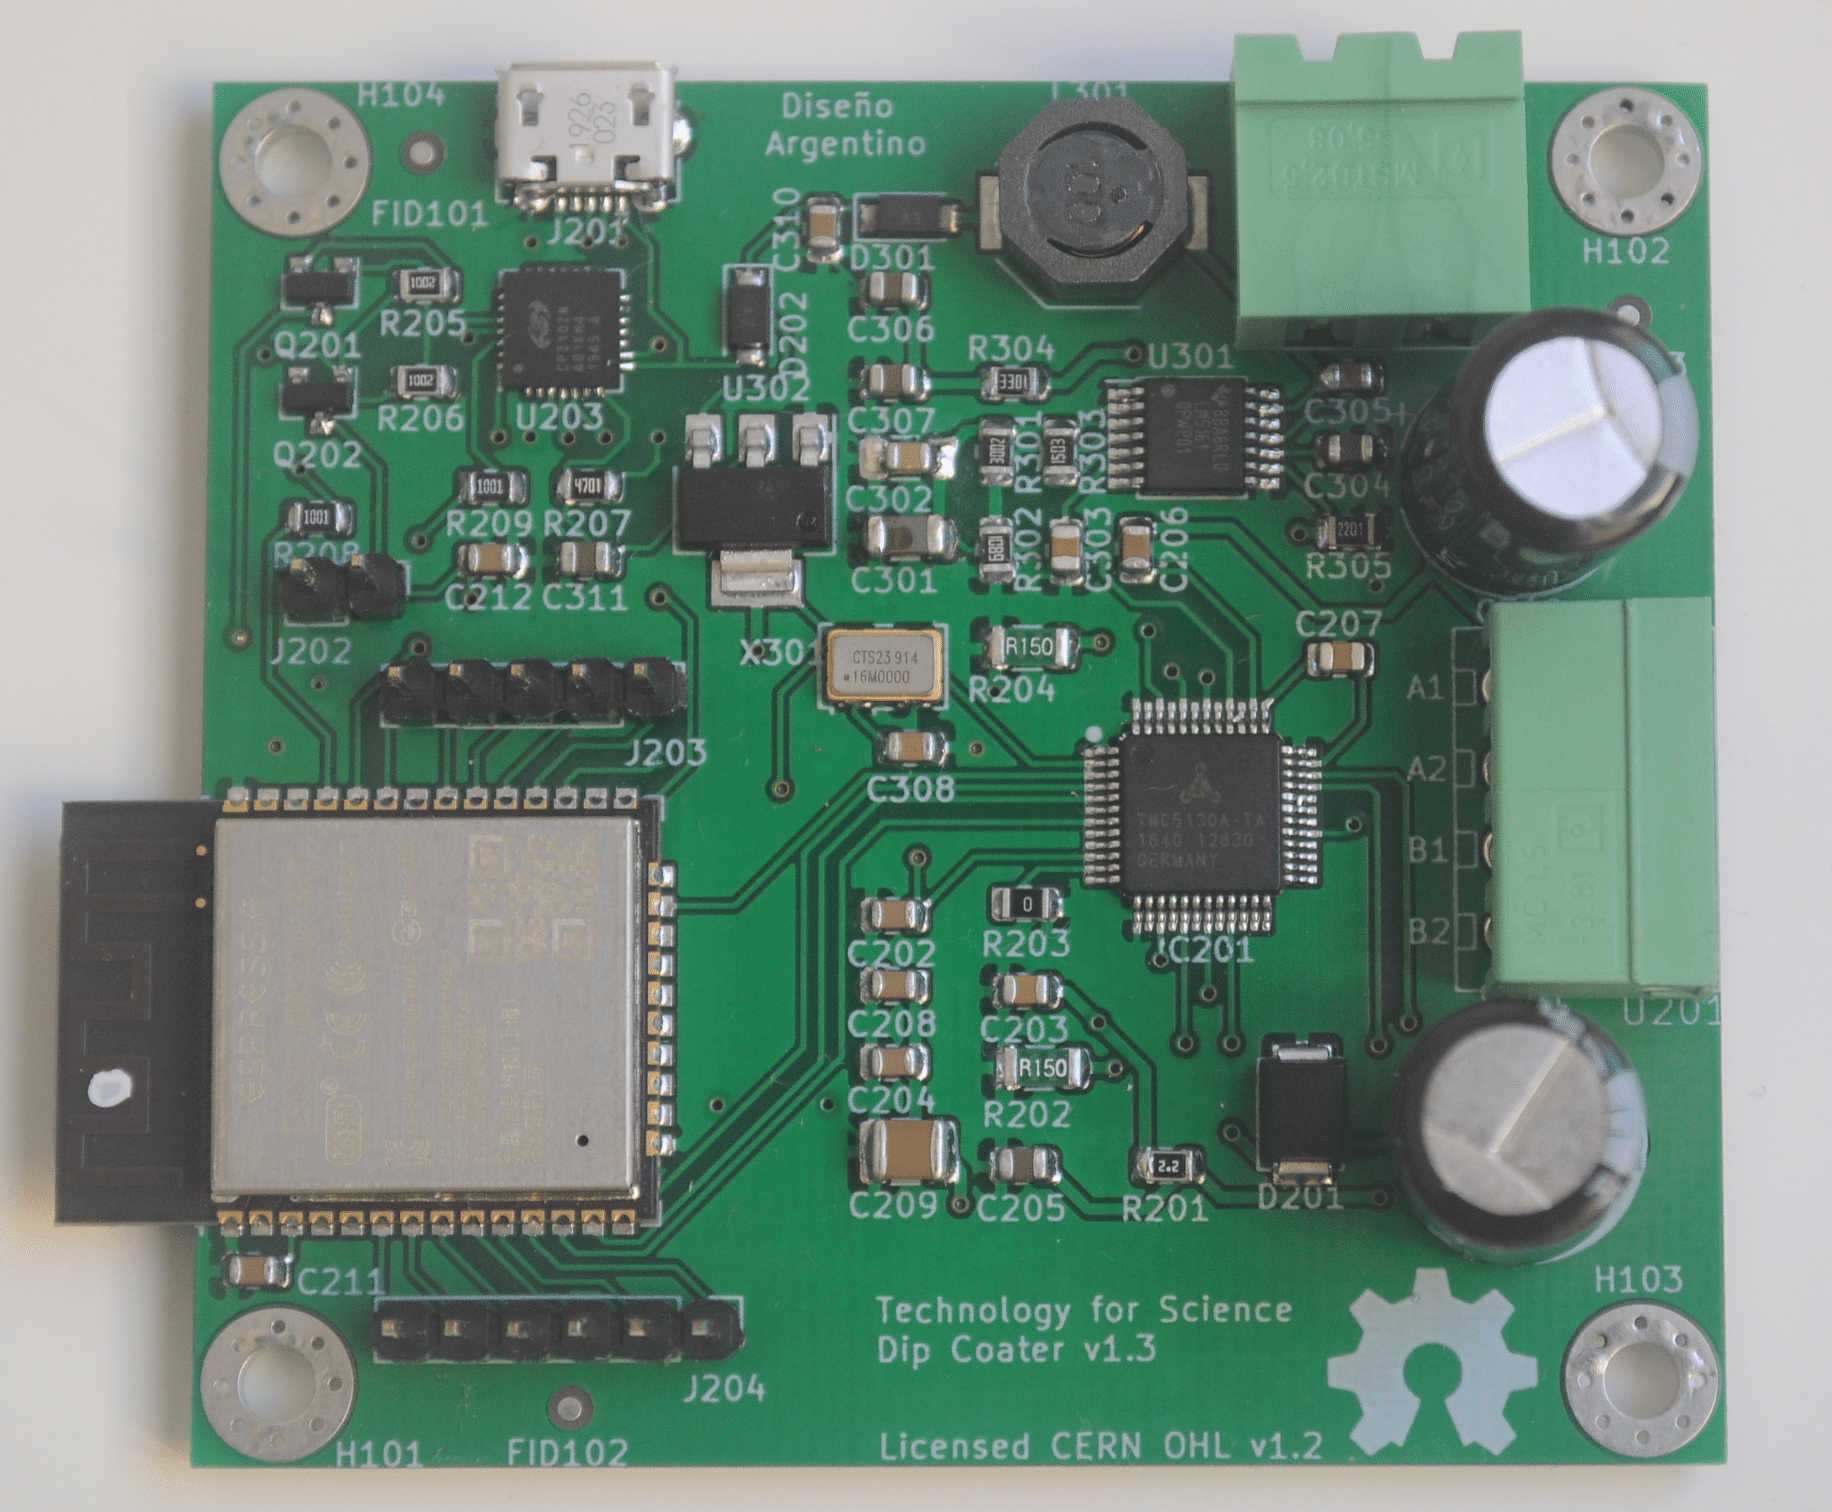
\includegraphics[width=0.6\textwidth]{./Figures/dip_real_model.jpg}
	\caption{Plaqueta electrónica final.}
	\label{fig:dip_real_model}
\end{figure}

%----------------------------------------------------------------------------------------
%	SECTION 2
%----------------------------------------------------------------------------------------

\section{Firmware}
\subsection{Capas de abstracción}

Se desarrolló un firmware modular que permite incorporar código de manera incremental y ordenada. Se observan en la figura \ref{fig:capas} las capas de abstracción de software implementadas. Esta implementación tiene dos ideas fundamentales:

\begin{itemize}
\item No se permite llamados a funciones entre capas discontinuas. Los módulos de la capa superior o capa APP solo pueden hacer llamados a funciones de la capa intermedia o capa API \textit{(Application Programming Interfaces)} y estas últimas solo pueden llamar a funciones de la capa inferior o capa BOARD.
\item Las aplicaciones pueden funcionar de manera independiente,  las mismas se pueden habilitar o deshabilitar.
\end{itemize}

\begin{figure}[h]
	\centering
	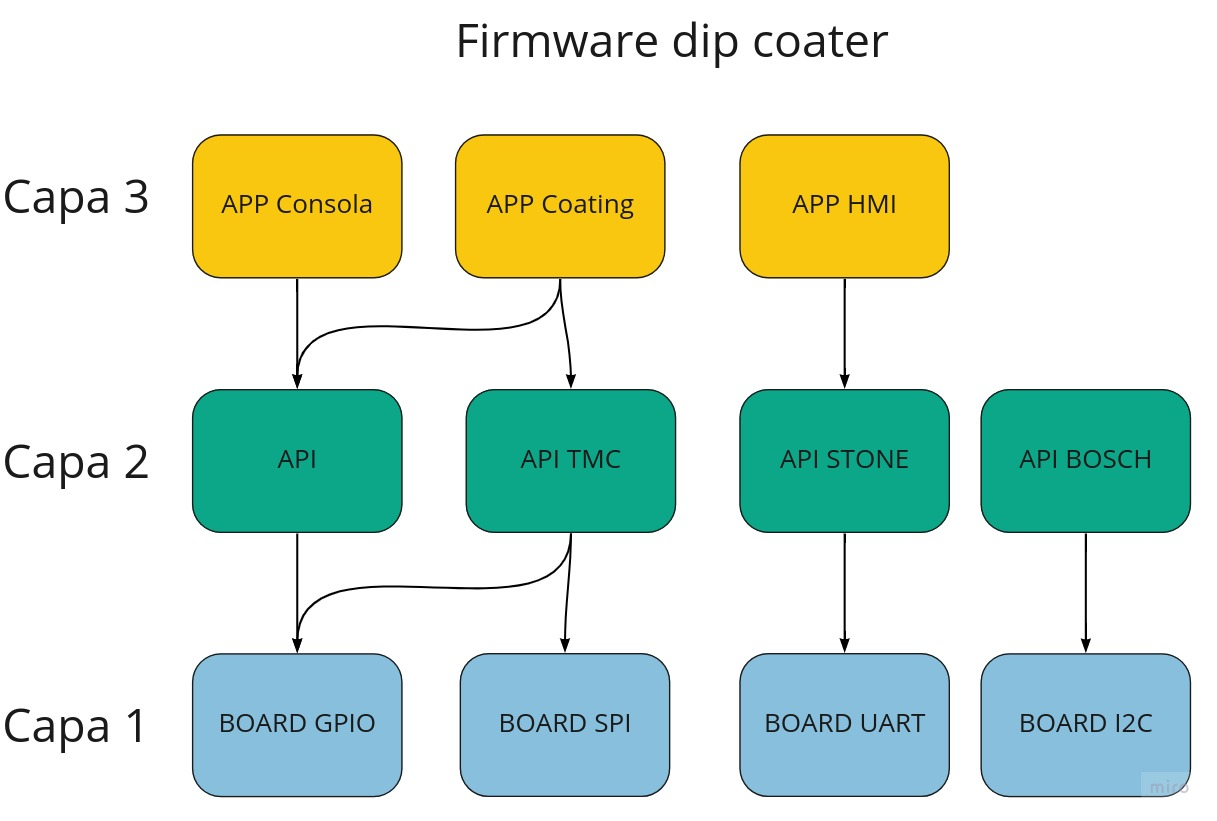
\includegraphics[width=1\textwidth]{./Figures/capas.jpg}
	\caption{Capas de abstracción de software.}
	\label{fig:capas}
\end{figure}


La capa tres corresponde a la capa de aplicaciones. El firmware cuenta con 3 aplicaciones fundamentales para el funcionamiento del equipo y una aplicación de testing utilizada para probar nuevos componentes de software. Cada aplicación contiene al menos una \textit{task} del sistema operativo freeRTOS. A continuación se detallan las aplicaciones:

\begin{itemize}

\item APP coating: se encarga de la comunicación con el driver TMC5130 y de la ejecución de todos los movimientos.
\item APP consola: administra una consola de comandos que permite ejecutar y configurar el equipo a través de una comunicación serial, recibe comandos en la consola serial y los envía a traves de una cola de freeRTOS a la app coating para ser procesados.
\item APP hmi: administra la interfaz de configuración, establece una comunicación serial con la pantalla táctil, recibe comandos a través de una cola de freeRTOS y los envía a la app coating para ser procesados.
\item APP test: se utiliza para probar nuevos componentes y realizar tests sobre el sistema. Se activa y desactiva según la necesidad de uso.

\end{itemize}
% y realizar test sobre el sistema que se activa y desactiva según la necesidad de uso.

La capa dos esta compuesta por bloques de código provistos por los fabricantes de drivers:
\begin{itemize}
\item API TMC: provista por el fabricante Trinamic y adaptada para ser ejecutada bajo el framework ESP-IDF.
\item API BOSH: provista por el fabricante y adaptada a este firmware.
\item API STONE: contiene los módulos de software que interaccionan con la pantalla táctil.
\item API: se utiliza como puente hacia la capa BOARD que tiene acceso a los periféricos del microcontrolador y con módulos de software del \textit{framework} ESP-IDF.

\end{itemize}

La capa uno es la que interacciona con los módulos de hardware del microcontrolador. Por lo tanto, esta capa es la única que contiene llamados a funciones disponibles en el framework ESP-IDF, como por ejemplo las funciones de configuración de los periféricos UART, GPIO, SPI, etc. Es importante mencionar que si debido a un rediseño se decide cambiar el microcontrolador utilizado, solo se deberán reescribir los módulos pertenecientes a esta capa y se podrá mantener el resto del programa sin alteraciones.

\subsection{Módulos principales de software}
\label{sec:modulos principales}

\subsubsection{Funcionamiento general}
 
App coating puede recibir a través de implementaciones de colas de FreeRTOS comandos de ejecución desde la app hmi y desde app consola.

Las aplicaciones app consola y app hmi se encargan de la interacción con el usuario y son las encargadas de enviar a la aplicación app coating los comandos para ejecutar los distintos movimientos.

El equipo dip coater puede ser utilizado de dos maneras diferentes detalladas a continuación:

\begin{enumerate}
\item A través de una consola de comandos.
\item A través de una pantalla táctil.
\end{enumerate}

Ambas opciones permiten ejecutar un ciclo completo de dip coating y también permiten ejecutar comandos de manera individual.
\subsubsection{Control de movimientos}

La aplicación app coating contiene toda la lógica de control de movimientos. La misma se encarga de realizar la configuración inicial del driver TMC5130, de ejecutar los procesos completos de dip coating y de procesar comandos individuales para generar diferentes tipos de acciones. 

Como se mencionó en la subsección \ref{subsection:Driver TMC5130} calcular los parámetros iniciales del driver es una tarea compleja, por lo que se optó por utilizar el software TMCL-IDE provisto por el fabricante y realizar la configuración de los registros de manera interactiva.

%Como se mencionó en la subsección \ref{subsection:Driver TMC5130} la configuración inicial del driver es compleja, por tal motivo se utilizo el software  TMCL-IDE provisto por el fabricante para obtener los valores de inicialización de los registros de manera interactiva.
%Cabe destacar que con este software se pueden configurar todos los driver que la compañía ofrece, abarcando desde motores paso a paso hasta  servomotores, motores \textit{brushless} y de corriente continua. 

En esta etapa de configuración es recomendable que el motor este acoplado al eje lineal, junto con el tornillo, la tuerca y el carro ya que el driver registra la corriente que circula por las bobinas del motor y calcula la fuerza contraelectromotriz que el eje esta ejerciendo. 
En la figura \ref{fig:tmcl_ide} se observa el entorno de desarrollo TMCL-IDE.  

\begin{figure}[h!t]
	\centering
	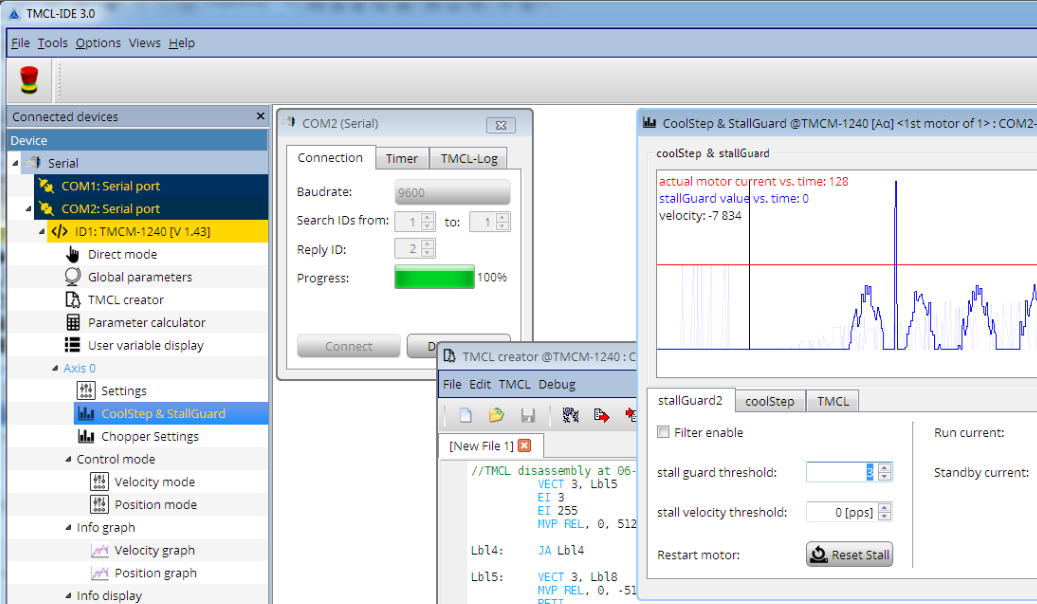
\includegraphics[width=1\textwidth]{./Figures/tmcl_ide_1.png}
	\caption{Software TMCL-IDE.}
	\label{fig:tmcl_ide}
\end{figure}


En la figura \ref{fig:tmcl_ide_stall} se puede observar el \textit{wizard} de configuración de las funciones \textit{stallguard2} y \textit{coolstep}.
Como se mencionó en el capítulo \ref{Chapter2} es posible usar stallguard2 para detectar los límites mecánicos de recorrido. El parámetro \textit{stall guard threshold} relaciona la fuerza contraelectromotriz registrada por el driver. A medida que se detecta mayor fuerza, es decir mayor oposición al movimiento y mayor corriente en los motores, el valor de stallguard2 disminuye. Se debe configurar entonces un valor límite de detección para que una vez alcanzado se genere un evento.

El firmware cuenta con una función llamada \textit{mod-coating-process-cero-machine} que se encarga de detectar el evento que el driver envía cuando se detecta un final de carrera. La misma se encarga de parar el motor, generar un desplazamiento en sentido contrario y establecer una nueva posición.

  

\begin{figure}[h!]
	\centering
	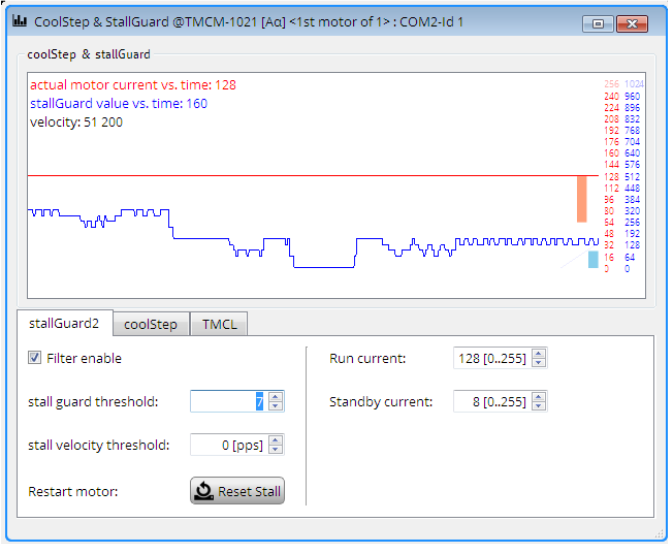
\includegraphics[width=0.6\textwidth]{./Figures/tmcl_ide_2.png}
	\caption{Configuración de funcionalidades stalldguard2 y coolstep.}
	\label{fig:tmcl_ide_stall}
\end{figure}

Otros parámetros importantes a configurar son los que definen la rampa de aceleración del desplazamiento. El driver permite configurar una rampa de seis puntos donde los valores a encontrar, A1, AMAX, D1, DMAX, V1 y VMAX corresponden a la aceleración, desaceleración y velocidad, como se observa en la figura \ref{fig:rampa}.



\begin{figure}[h!]
	\centering
	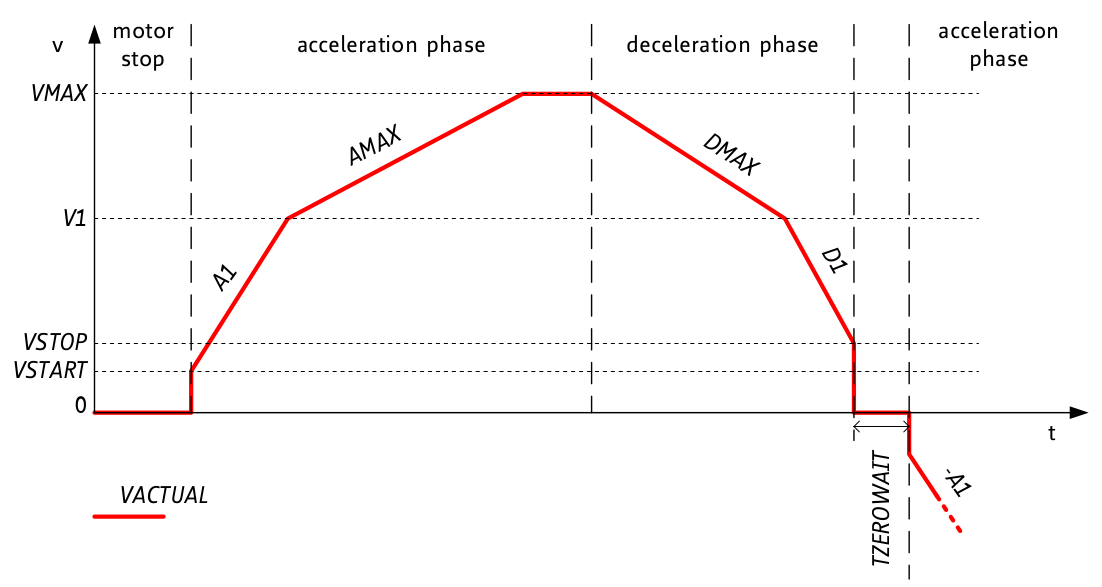
\includegraphics[width=0.8\textwidth]{./Figures/rampa_1.png}
	\caption{Configuración de rampa de seis puntos.}
	\label{fig:rampa}
\end{figure}


%Todos los movimientos del equipo dip coater están definidos de la siguiente manera \ref{cod:vControl_1}.
%\begin{lstlisting}[label=cod:vControl_1,caption=Macros para configurar de desplazamientos.] 
%	// Velocidad
%	//V1
%	Evalboards.ch1.writeRegister(0, TMC5130_V1, (arg->velocity) / 2);
%	//VMAX
%	Evalboards.ch1.writeRegister(0, TMC5130_VMAX, arg->velocity);
%	//VSTART
%	Evalboards.ch1.writeRegister(0, TMC5130_VSTART, 0);
%	//VSTOT
%	Evalboards.ch1.writeRegister(0, TMC5130_VSTOP, 100);
%
%	// Seteo Aceleracion
%	//A1
%	Evalboards.ch1.writeRegister(0, TMC5130_A1,  arg->acceleration);
%	//AMAX
%	Evalboards.ch1.writeRegister(0, TMC5130_AMAX,  arg->acceleration);
%
%	// Seteo Desaceleracion
%
%	//DMAX
%	Evalboards.ch1.writeRegister(0, TMC5130_DMAX,  arg->acceleration);
%	//D1
%	Evalboards.ch1.writeRegister(0, TMC5130_D1,  arg->acceleration);
%\end{lstlisting}

Para el control de los movimientos se optó por generar una rampa de cuatro puntos que el usuario puede configurar según lo desee. Se implementó entonces la siguiente relación de variables:

\begin{itemize}
\item A1 = AMAX  (Aceleración establecida por usuario).
\item D1 = DMAX  (Desaceleración establecida por usuario).
\item VMAX 	  (Velocidad establecida por usuario).
\item V1 = VMAX / 2 (Velocidad fija del movimiento).

\end{itemize}

\subsubsection{Consola de comandos}

App consola permite establecer un canal de comunicación entre el equipo dip coater y un ordenador a través de una comunicación serial. Como se mencionó en la subsección \ref{subsection:Diseño basado en módulos de hardware libre}, la placa electrónica incorpora un conversor serie TTL-USB que permite conectar el  equipo directamente a través de un cable USB. 

Se definen dos series de comandos:
\begin{itemize}
\item Los que permiten ejecutar un proceso completo de dip coating y están pensados para ser utilizados por un usuario.
\item Los que permiten realizar consultas y configuraciones sobre el sistema y fueron utilizados durante el desarrollo del trabajo.
\end{itemize}



\begin{figure}[h!]
	\centering
	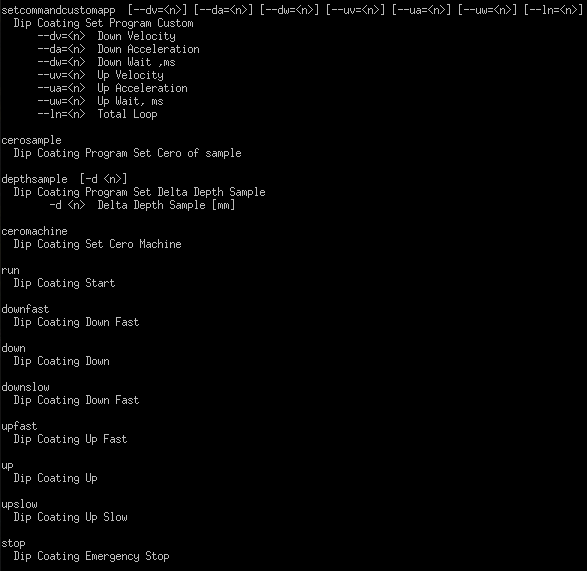
\includegraphics[width=1\textwidth]{./Figures/consola_2.png}
	\caption{Comandos de movimientos.}
	\label{fig:consola_movimientos}
\end{figure}

En la figura \ref{fig:consola_movimientos} se observa la primer serie de comandos. El comando setcommandcustomapp permite configurar los siguientes parámetros del proceso:

\begin{itemize}
\item Velocidad y aceleración ascendente y descendente.
\item Tiempos de espera en posición superior e inferior.
\item Cantidad de repeticiones del ciclo.
\end{itemize}

El comando cerosample permite configurar la posición inicial donde comienzo el movimiento. El comando depthsample permite configurar la distancia de recorrido de la muestra. Para ejecutar el proceso, con los párametros anteriores  establecidos, se debe ejecutar el comando run. También esta disponible el comando stop para que el usuario pueda detener el proceso si así lo desea. El resto de los comandos  down, downfast, up, etc, permiten movimientos individuales que sirven para posicionar la muestra.

Se observa en la figura \ref{fig:consola_comandos} la segunda serie de comandos. Los comandos read-register y write-register sirven para leer y escribir registros del driver TMC5130. El comando data permite leer todos los parámetros del proceso cargados en el sistema.



\begin{figure}[h!]
	\centering
	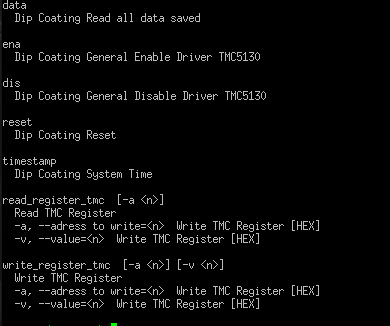
\includegraphics[width=0.7\textwidth]{./Figures/consola_3.png}
	\caption{Comandos de control.}
	\label{fig:consola_comandos}
\end{figure}

A modo de ejemplo se observa en la figura \ref{fig:comando_lectura} una consulta sobre el registro Xactual[0x21], que expresa la posición actual en micro pasos desde la referencia inicial y otra consulta sobre el registro Xtarget[0x2D], cuyo valor expresa la posición objetivo en micro pasos que se desea alcanzar. En este ejemplo Xactual = Xtarget ya que el equipo estaba detenido. Para ejecutar un movimiento se debe configurar una posición en Xtarget que accionara el motor hasta alcanzar Xactual = Xtarget.


\begin{figure}[h!]
	\centering
	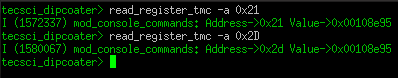
\includegraphics[width=1\textwidth]{./Figures/consola_6.png}
	\caption{Lectura de registros del driver TMC5130.}
	\label{fig:comando_lectura}
\end{figure}


Cada vez que el usuario ejecuta un comando sobre la consola, la aplicación app console procesa y envía el mensaje a través de una cola de FreeRTOS hacia la aplicación app coating. Si la máquina está ejecutando un movimiento individual o un proceso dip coating completo y recibe un comando nuevo, el mismo por seguridad es descartado, es decir que los mensajes no se encolan. En la figura 
\ref{fig:consola_comando_ok} se observa que luego de iniciar el proceso dip coating se envía el comando DOWN y el mismo es descartado sin afectar el proceso.

\begin{figure}[h!]
	\centering
	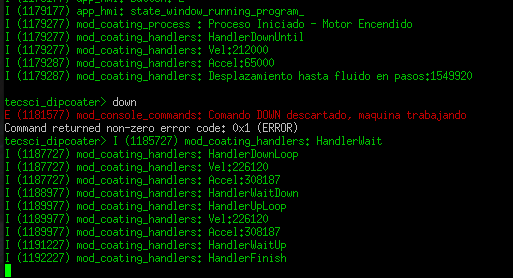
\includegraphics[width=1\textwidth]{./Figures/consola_4.png}
	\caption{Comando DOWN descartado por equipo en funcionamiento.}
	\label{fig:consola_comando_ok}
\end{figure}

El único comando de movimiento que no es descartado es el comando STOP, el cual tiene un tratamiento especial y siempre se garantiza su ejecución.

\begin{figure}[h!]
	\centering
	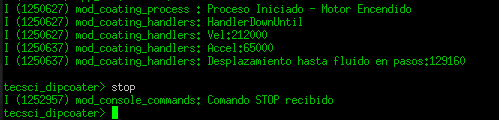
\includegraphics[width=1\textwidth]{./Figures/consola_5.png}
	\caption{Comando STOP procesado.}
	\label{fig:consola_comando_false}
\end{figure}

\subsubsection{Pantalla táctil}

La aplicación app hmi establece un canal de comunicación serial entre la pantalla táctil y el microcontrolador, la misma se encarga de procesar datagramas salientes y entrantes. 

En la sección \ref{sec:interfaz_pantalla} se presentó el modelo STWI043WT elegido para el equipo dip coater, el mismo requiere para su configuración el desarrollo de un proyecto con el software \textit{STONE GUI Desing Software}. En la figura \ref{fig:stone_a} se presenta la interfaz interactiva que permite crear pantallas y diferentes tipos de objetos o \textit{widgets} para brindar de funcionalidad a las mismas. El fabricante define también un protocolo de comunicación \citep{web_protocolo_stone} para interaccionar con los objetos que componen cada pantalla.

\begin{figure}[h!]
	\centering
	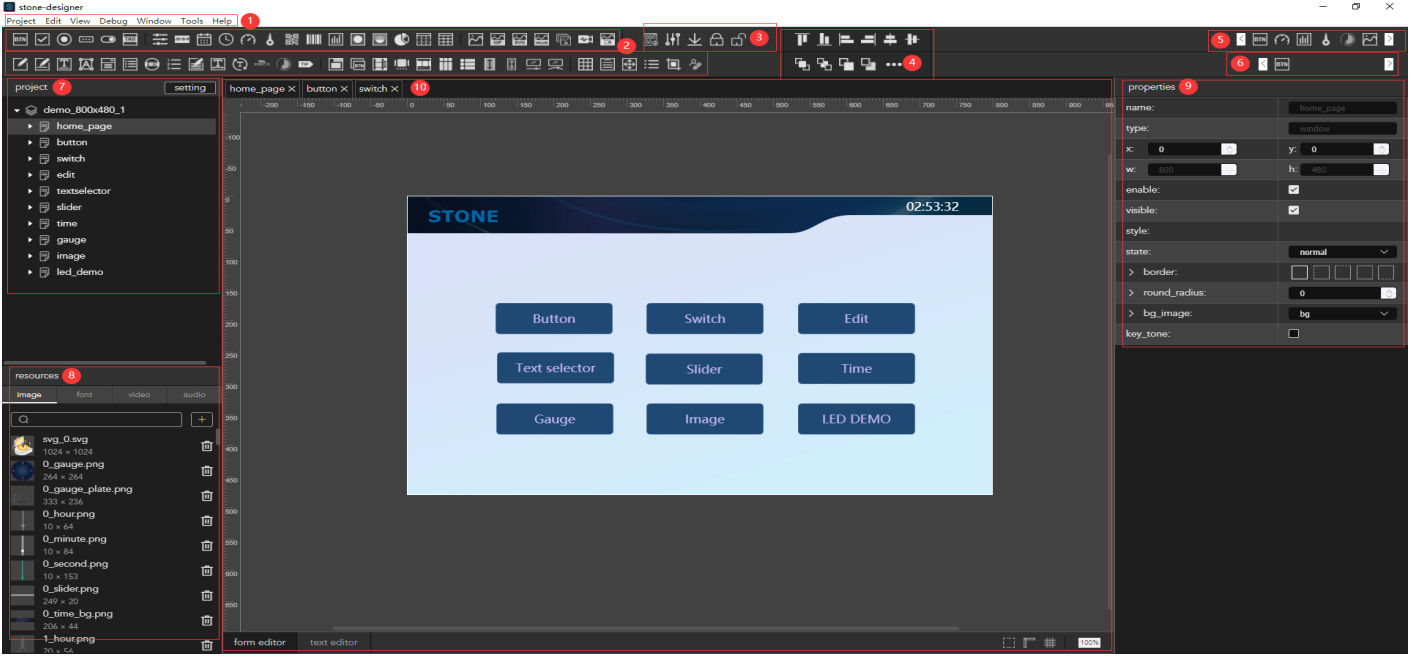
\includegraphics[width=1\textwidth]{./Figures/stone_a.png}
	\caption{STONE GUI Desing Software.}
	\label{fig:stone_a}
\end{figure}



En la figura \ref{fig:datagrama_a} se define el formato de datagrama para enviar datos desde el microcontrolador hacia la pantalla. 

\begin{figure}[h!]
	\centering
	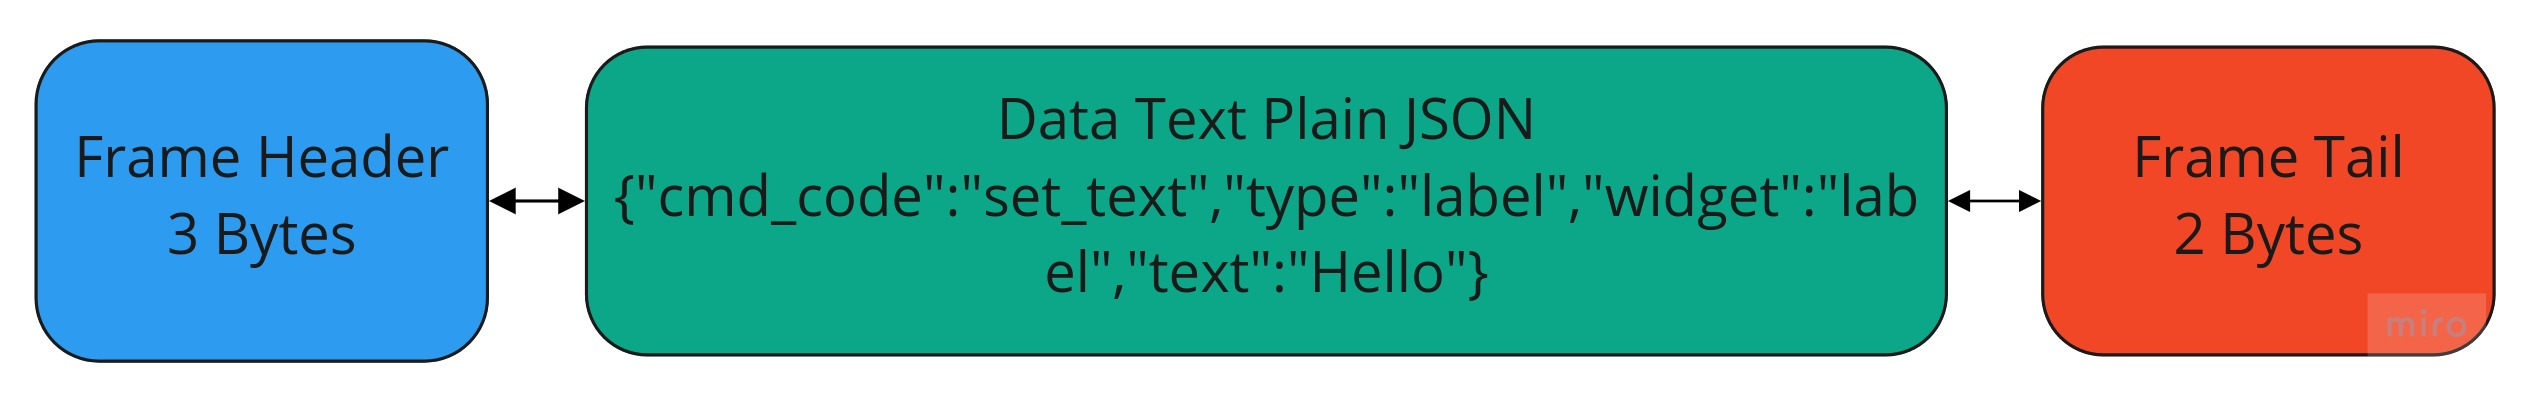
\includegraphics[width=1\textwidth]{./Figures/datagrama_b.jpg}
	\caption{Datagrama desde microcontrolador hacia pantalla.}
	\label{fig:datagrama_b}
\end{figure}

El datagrama está compuesto por tres bloques:
\begin{enumerate}
\item Frame header: 3 bytes fijos.
\item Data: Datos definidos en texto plano con formato \textit{JSON (JavaScript Object Notation)}.
\item Frame tail: 2 bytes fijos.
\end{enumerate}

El campo data define múltiples categorías, se mencionan a continuación las mas importantes:
\begin{itemize}
\item Cmd-code: Es un identificador único que define la instrucción.
\item Type: Define el tipo de objeto.
\item Widget: Define el nombre único del objeto.
\item Text: Define el contenido del objeto, varia según el tipo de objeto.
\end{itemize}  

En la figura \ref{fig:datagrama_a} se define el formato de datagrama para enviar datos desde la pantalla hacia el microcontrolador. El datagrama esta compuesto por los siguientes bloques:

\begin{figure}[h!]
	\centering
	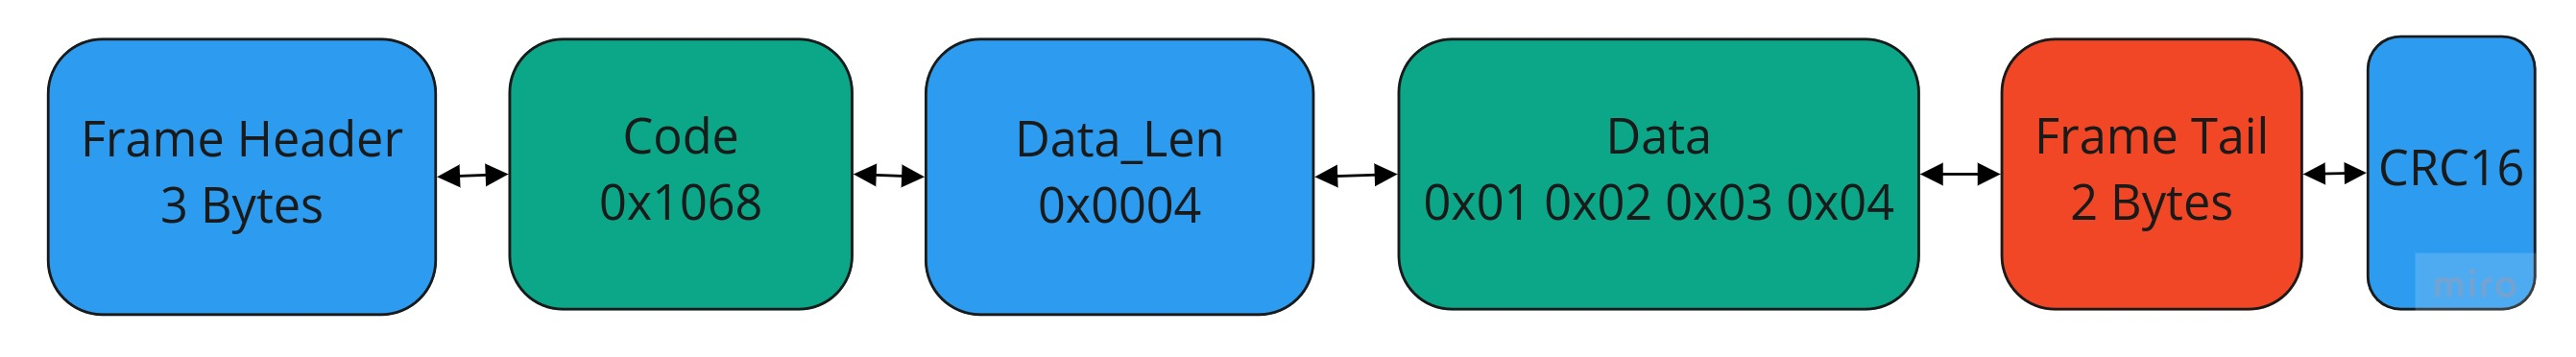
\includegraphics[width=1\textwidth]{./Figures/datagrama_a.jpg}
	\caption{Datagrama desde pantalla hacia microcontrolador.}
	\label{fig:datagrama_a}
\end{figure}

\begin{enumerate}

\item Frame header: 3 bytes fijos.
\item Code: Identificación única de objeto.
\item Data-Len: Define el largo del dato a transmitir.
\item Data: Su tamaño debe coincidir con el item anterior.
\item Frame tail: 2 bytes fijos.
\item CRC16: Para verificación de integridad del datagrama.

\end{enumerate}

Para procesar los datagramas entrantes se implementó un bloque de código que analiza el buffer del periférico UART-1. Cuando hay datos disponibles el periférico envía un evento a través de una \textit{queue} de freeRTOS. El evento UART-DATA se recibe en la \textit{task} mod-hmi-RX-task-loop la cual comienza a procesar dichos datos mientras estén disponibles. En la figura \ref{fig:secuencia_a} se observa el control que se va realizando a cada unos del los bytes entrantes. Si el datagrama pasa todas las condiciones es aceptado y enviado a la \textit{task} app hmi task a través de una \textit{queue} para ser procesado.


\begin{figure}[h!]
	\centering
	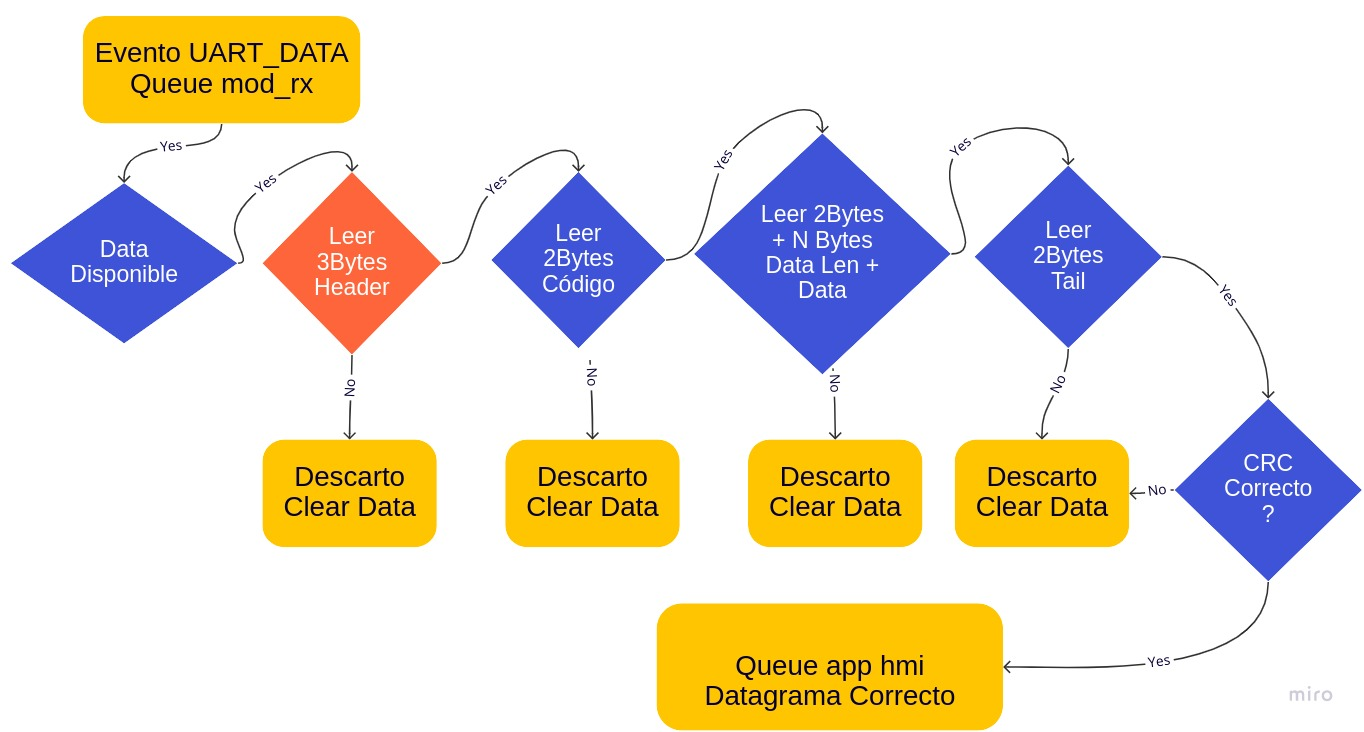
\includegraphics[width=\textwidth]{./Figures/Secuencia_lectura_uart.jpg}
	\caption{Secuencia de procesamientos de datos entrantes.}
	\label{fig:secuencia_a}
\end{figure}

 
En la figura \ref{fig:stone_a} se presenta la pantalla de configuración de programa  creada con el software de diseño.

\begin{figure}[h!]
	\centering
	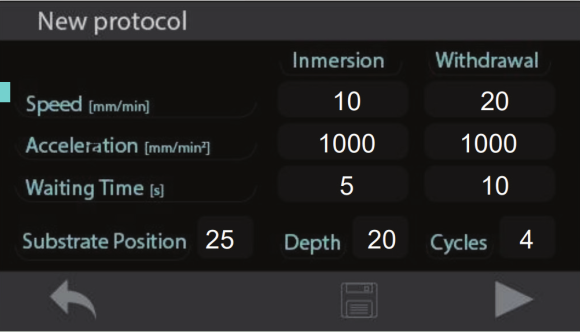
\includegraphics[width=0.7\textwidth]{./Figures/pantalla.png}
	\caption{Pantalla de configuración de programa.}
	\label{fig:stone_a}
\end{figure}  


 

\subsubsection{Registros de variables ambientales}

En la sección \ref{sec:sistema_propuesto} se presentó el requerimiento opcional que establece el registro de variables de humedad, presión y temperatura. El interés del cliente se fundamenta en que ciertos experimentos necesitan realizarse particularmente a humedad y temperatura controlada. 

Para el registro de estas variables se incorporó al sistema un sensor BME280, el mismo integra en un solo CI sensores de presión atmosférica, temperatura y humedad relativa. El fabricante ofrece en sus repositorios \citep{web_repositorio_api_bosh} ejemplos de implementaciones y una API para utilizar todas las funcionalidades del CI.

La comunicación entre el sensor y el microcontrolador se realizó a través del protocolo I2C, se incorporó el módulo del software BOARD I2C que se encarga de inicializar el periférico. También se implementó el módulo API BOSH BME, que trabaja con todas las funcionalidades que ofrece el fabricante en su API. En la figura \ref{fig:api_bosh} de observa el flujo de capas desarrollado:

\begin{figure}[h!]
	\centering
	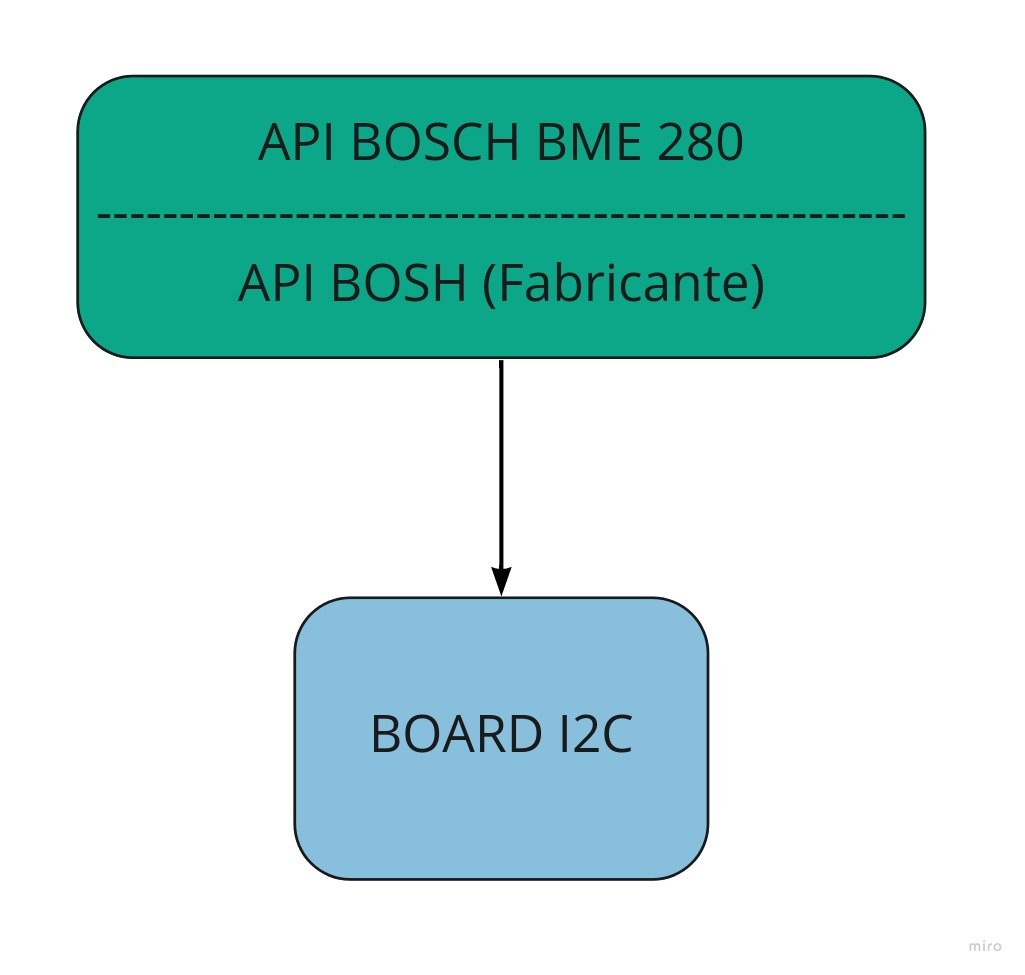
\includegraphics[width=0.4\textwidth]{./Figures/api_bosh_bme.jpg}
	\caption{Módulo API BOSH.}
	\label{fig:api_bosh}
\end{figure}

API BOSH BME inicializada una estructura donde define los siguientes parámetros de interés:
\begin{itemize}
\item Dirección del dispositivo I2C.
\item Función de lectura.
\item Función de escritura.
\item Función de delay.
\item Configuración de modo normal de funcionamiento del sensor. 
\end{itemize}

Para visualizar los datos registrados por el sensor se implementó sobre la APP TEST una rutina de consulta con llamado a funciones de la capa API BOSH BME, se observa en la siguiente figura los datos registrados en consola.

\begin{figure}[h!]
	\centering
	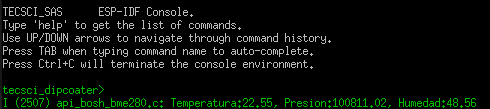
\includegraphics[width=1\textwidth]{./Figures/registro_bme.png}
	\caption{Registro de datos en consola.}
	\label{fig:api_bosh}
\end{figure}

 
El desarrollo de este MPV incluyó el registro de variables ambientales pero no un control y corrección de las mismas con un sistema de control. Sin embargo, se pretende ofrecer en un futuro cercano la funcionalidad de cámara de humedad anexada a este MPV. Por tal motivo se presenta en el anexo XX el desarrollo de un sistema de control de humedad.  

\subsubsection{Parámetros de calibración}
\label{subsec:calibracion}

La carpeta /components/config contiene tres archivos de configuración importantes:
\begin{itemize}
\item hardware.h: contiene todas las macros referidas a los pines de conexión del modelo de microcontrolador utilizado.
\item os-config.h: contiene las macros de configuración de las tareas y colas de FreeRTOS. Entre otras los tamaños de stack, las prioridades y los periodos de tiempo de ejecución de tareas.
\item machine.h: contiene las macros relacionadas con la calibración mecánica del equipo.
\end{itemize}


La macro más importante configurada en el archivo machine.h es MACHINE STEPS PER MILLIMETER y es necesario que este bien definida. En la sección \ref{sec:calibración} se demuestra el procedimiento realizado para definir su valor. Esta macro define la cantidad de micro pasos necesarios para generar el desplazamiento de 1 mm. La misma esta completamente relaciona con el paso del tornillo acoplado al eje del motor. Las unidades de posición son expresados en micro pasos, las unidades de velocidad en micro pasos sobre segundos y las unidades de aceleración en micro pasos sobre segundos al cuadrado.

Se observa en la figura \ref{fig:unidades}, extraída de la hoja de datos del driver TMC5130, los factores de corrección que deben aplicarse cuando se cuenta con un clock externo incorporado en el circuito electrónico. Se deben calcular las constantes que corrigen los valores de velocidad y aceleración.

\begin{figure}[h!]
	\centering
	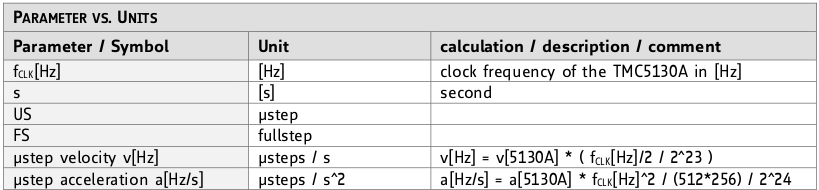
\includegraphics[width=1\textwidth]{./Figures/unit.png}
	\caption{Unidades.}
	\label{fig:unidades}
\end{figure}


Como se mencionó en la subsección \ref{subsection:Driver TMC5130} el equipo se configuró con 51200 micro pasos por vuelta completa.  
 
 

\begin{lstlisting}[label=cod:vControl,caption=Macros de desplazamiento y factores de conversión.]  % Start your code-block
/*Buscar este numero con calibración mecánica del sistema*/

#define MACHINE_STEPS_PER_MILLIMETER	(12916)		
#define MACHINE_EXT_CLOCK					(16000000)	//16MHz


/*FACTOR*/
/*((MACHINE_EXT_CLOCK/2)*(1/8388608))*/	
#define MACHINE_USTEPS_VELOCITY_FACTOR	  (0.9536743164)
/*((MACHINE_EXT_CLOCK*MACHINE_EXT_CLOCK)/(512*256)/ (16777216) )*/
#define MACHINE_USTEPS_ACELERATION_FACTOR (116.4153218)


/*UPPER AND LOWER MECHANICAL LIMIT*/

#define MACHINE_CONTROL_MECANICAL_UPPER_LIMIT 	(MACHINE_STEPS_PER_MILLIMETER * 10 ) // 10mm
#define MACHINE_CONTROL_MECANICAL_LOWER_LIMIT	(MACHINE_STEPS_PER_MILLIMETER * 290) // 290mm

\end{lstlisting}






%----------------------------------------------------------------------------------------
%	SECTION 3
%----------------------------------------------------------------------------------------

\section{Estructura mecánica}
\subsection{Fabricación de piezas personalizadas a través de mecanizado CNC}

\subsubsection{Etapa CAD}

Como se mencionó en la sección \ref{sec:estructura_mecanica} se utilizó para el diseño mecánico del equipo el software BOBCAD. El módulo CAD del software permite realizar modelos 2D y 3D de piezas.

El prototipo dip coater cuenta actualmente con dos piezas mecanizadas en aluminio. Se observa en la figura \ref{fig:carro} la pieza que se acopla al carro de la guiá lineal presentada en la sección \ref{sec:estructura_mecanica}.

\begin{figure}[ht]
	\centering
	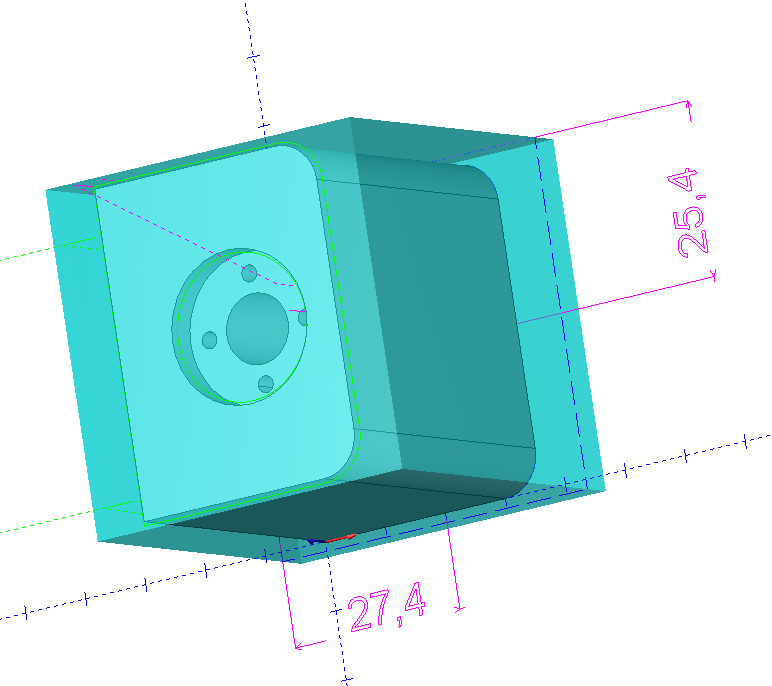
\includegraphics[width=.5\textwidth]{./Figures/3d_carro.png}
	\caption{Pieza personalizada soporte de carro.}
	\label{fig:carro}
\end{figure}

Y en la figura \ref{fig:estructura_superior} el soporte superior que sostiene el motor paso a paso y el  tornillo acoplado al eje del motor.

\begin{figure}[h]
	\centering
	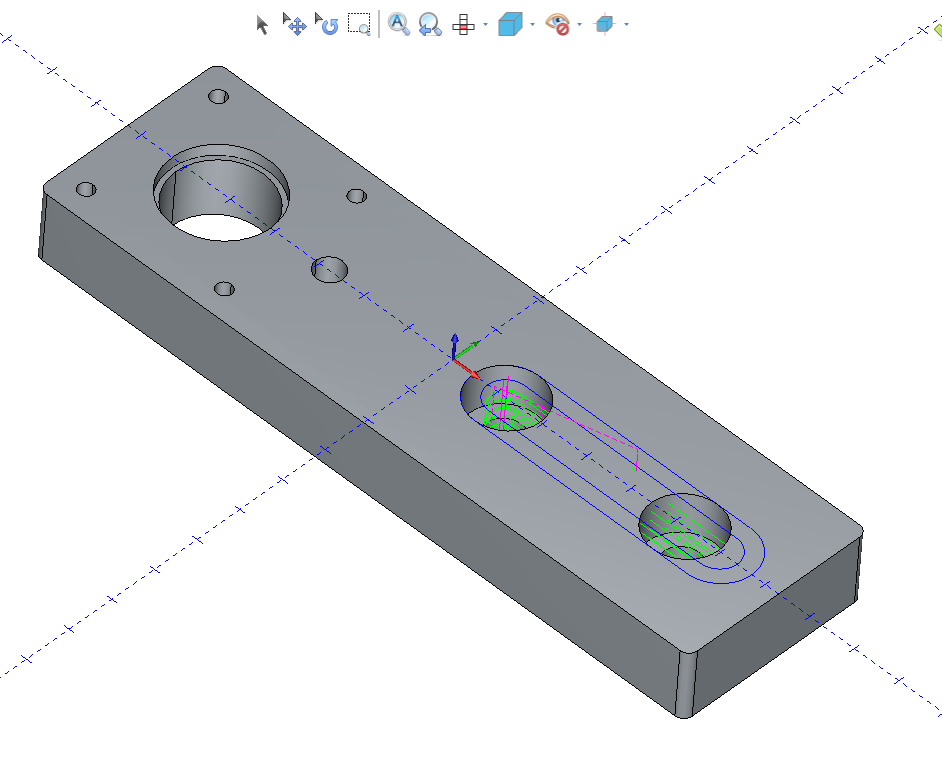
\includegraphics[width=.5\textwidth]{./Figures/3d_top.png}
	\caption{Piezas personalizada soporte de estructura superior.}
	\label{fig:estructura_superior}
\end{figure}

Con los modelos 3D diseñados, se fabricaron primeras versiones a través de impresión 3D en plástico. 
Luego que las piezas fueron probadas, testeadas y aprobadas en el prototipo, se pasó a la fabricación final sobre aluminio.

\subsubsection{Etapa CAM}

La estrategia utilizada en el mecanizado CNC es por el método de arranque de viruta. Este consiste en partir de un bloque de aluminio con volumen de material suficiente y desbastar con herramientas de corte hasta modelar la pieza. Esta estrategia se programa en la parte CAM del software. Existen diferentes operaciones de mecanizado que se utilizan según el tipo de pieza que se desee fabricar. Tal es el caso de refrentado, vaciado, fresado de chaflán, taladrado y roscado entre otras. Cada una de estas operaciones  en general se realizan con herramientas específicas que son definidas en la configuración del software.

A modo de ejemplo se presenta en la figura \ref{fig:estrategia} el listado de operaciones realizadas para la fabricación de una de las piezas del dip coater.

\begin{figure}[h]
	\centering
	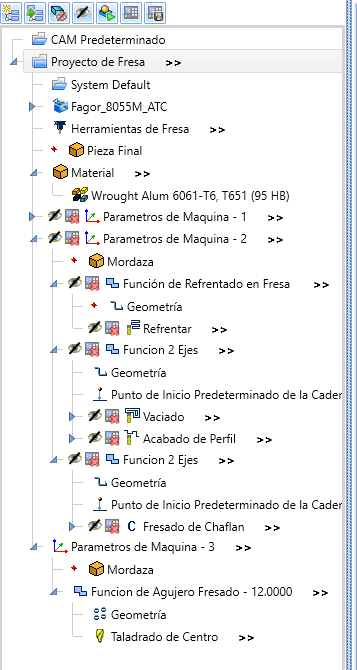
\includegraphics[width=.6\textwidth]{./Figures/3d_estrategia.png}
	\caption{Operaciones de mecanizado en software Bodcad.}
	\label{fig:estrategia}
\end{figure}

En general las piezas se fabrican en dos etapas, primero a través de diferentes operaciones se mecaniza la parte superior, luego se rota la pieza 180° y se mecaniza la parte inferior.


El material mecanizado para la fabricación de estas piezas fue aluminio 6061, el mismo es una aleación endurecida compuesta por aluminio, magnesio y silicio. La elección se basó en que el mismo puede someterse a tratamientos de anodizado posteriores. El anodizado es un tratamiento electrolítico, que genera una capa superficial de óxido de aluminio (alúmina). De espesor superior que el aluminio en estado natural, tiene como ventajas la protección contra atmósferas agresivas, agentes químicos y una mayor dureza superficial.

Finalmente en la figura \ref{fig:real_custom} se observan ambas piezas fabricadas.

\begin{figure}[h]
	\centering
	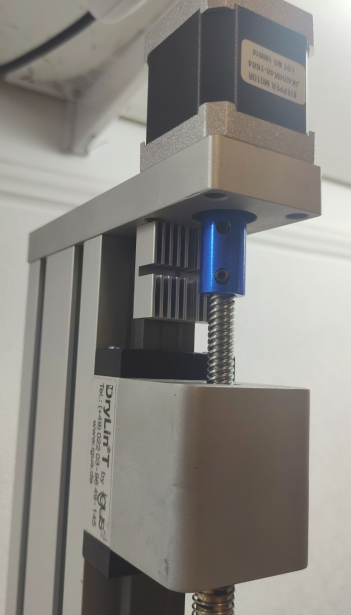
\includegraphics[width=0.5\textwidth]{./Figures/real_custom.png}
	\caption{Piezas fabricadas en centro de mecanizado.}
	\label{fig:real_custom}
\end{figure}


\subsection{Modelos 3D y real}

En la figura \ref{fig:mecanica_3d_model} se presenta el primer modelo 3D diseñado del equipo dip coater.
\begin{figure}[h]
	\centering
	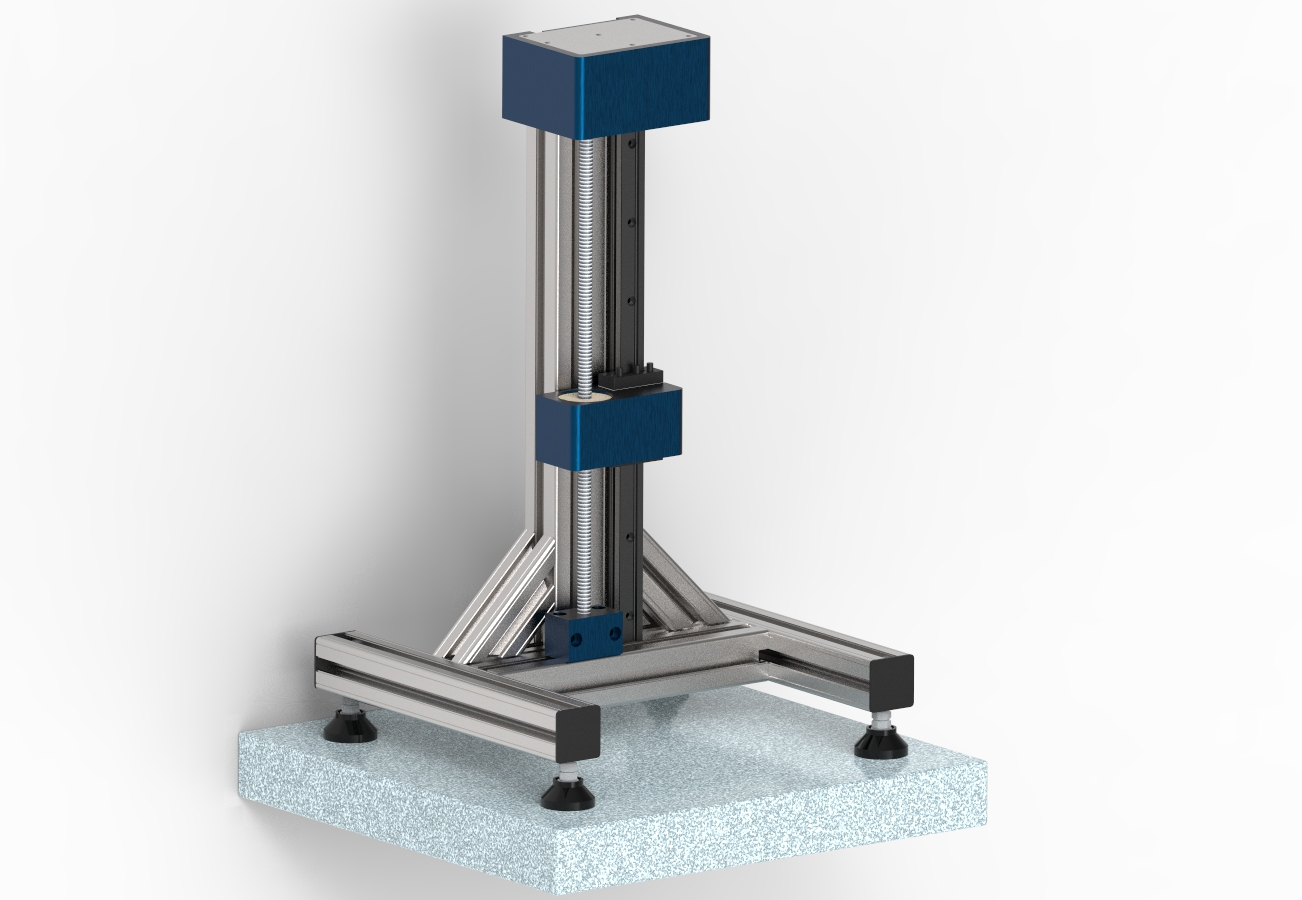
\includegraphics[width=0.9\textwidth]{./Figures/3d.jpg}
	\caption{Modelo 3D.}
	\label{fig:mecanica_3d_model}
\end{figure}


%Se detallan a continuación los siguientes componentes fundamentales del equipo:
%\begin{itemize}
%\item Guiás lineales IGUS 
%\item Mecanizado soporte superior y mecanizado carro
%\item Placa electrónica
%\item Pantalla táctil 4.3 inch
%\end{itemize}

Luego de sucesivas iteraciones con pruebas de piezas impresas en material plástico se logró fabricar un primer prototipo completamente en metal que se presenta en la figura \ref{fig:mecanica_real_model}.

\begin{figure}[h]
	\centering
	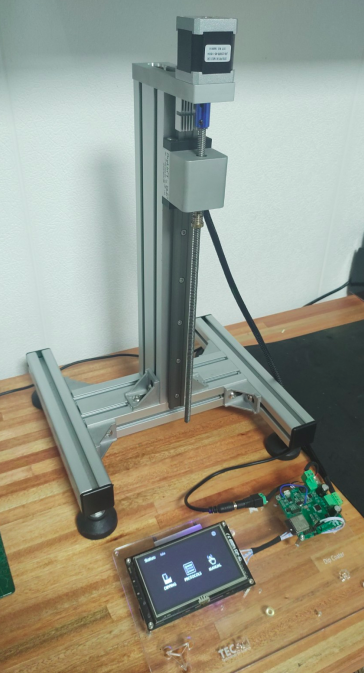
\includegraphics[width=0.4\textwidth]{./Figures/real.png}
	\caption{Primer prototipo dip coater TECSCI.}
	\label{fig:mecanica_real_model}
\end{figure}


% Chapter Template

\chapter{Ensayos y resultados} % Main chapter title

\label{Chapter4} % Change X to a consecutive number; for referencing this chapter elsewhere, use \ref{ChapterX}

%----------------------------------------------------------------------------------------
%	SECTION 1
%----------------------------------------------------------------------------------------

\section{Pruebas funcionales de hardware}
%\label{sec:pruebasHW}

En el presente capítulo se explican los ensayos realizados sobre el prototipo del equipo dip coater, se presentan y analizan los resultados obtenidos y se introducen posibles cambios para próximas versiones.
\subsection{Comunicación con driver TMC5130}

El presente ensayo se realizó para verificar la comunicación entre el microcontrolador ESP32 y el CI TMC5130. Como se mencionó en el capítulo \ref{Chapter3} dicha comunicación se establece a través del  protocolo SPI. En la figura \ref{fig:ensayo_spi_0} se observa el esquema del banco de pruebas propuesto.

\begin{figure}[h]
\centering 
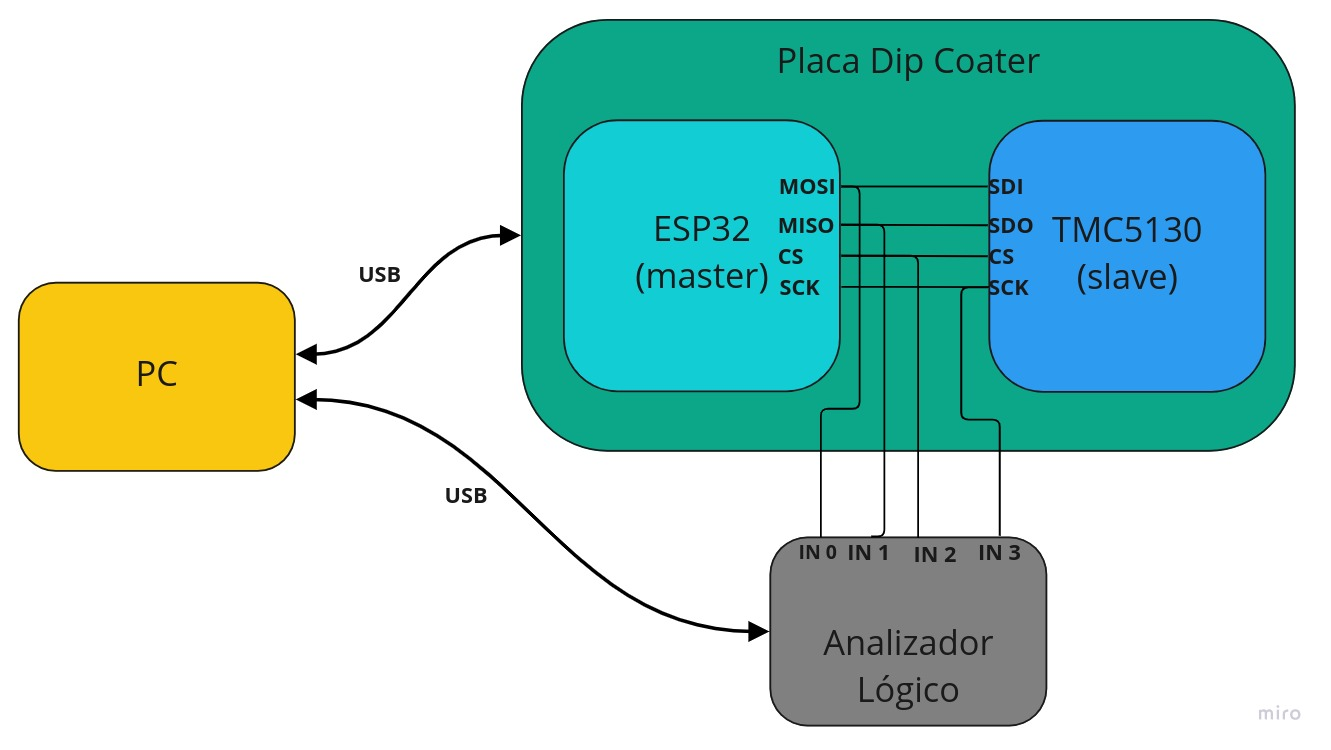
\includegraphics[width=1\textwidth]{./Figures/ensayo_spi.jpg}
\caption{Banco de pruebas.}
\label{fig:ensayo_spi_0}
\end{figure}


 
% Al encender el equipo se realiza una configuración inicial en donde se escriben todos los registros y luego durante el uso del equipo se realizan operaciones de lectura y escritura para conocer el estado del CI y accionar diferentes tipos de movimientos.
%Se configura el ESP como dispositivo \textit{SPI master} y el TMC5130 como dispositivo \textit{SPI slave}.

%En la figura \ref{fig:datagrama} se observa la estructura de datos para leer y escribir registros.
%\begin{figure}[h]
%\centering 
%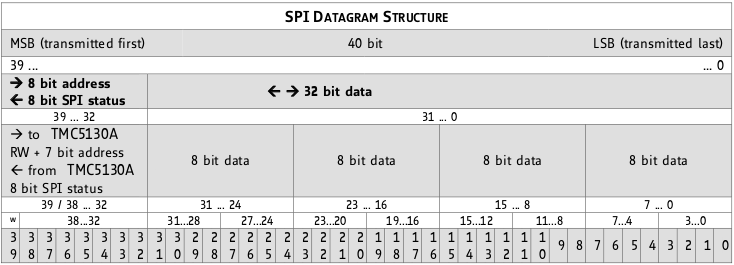
\includegraphics[width=1\textwidth]{./Figures/datagrama.png}
%\caption{Datagrama de 40 bits.}
%\label{fig:datagrama}
%\end{figure}


%Las operaciones de lectura y escritura tienen una diferencia, que se ve representada por el bit más significativo de la trama de datos, es decir el bit 39. Cuando la operación es de lectura, y primer byte que representa la dirección del registro no sufre alteración. Cuando la operación es de escritura, se debe establecer en 1 el bit de la posición 39. Por ejemplo, si  se pretende escribir un valor en el registro [0x22], el primer byte del datagrama deberá ser [0x22 + 0x80 = 0xA2],  sumar [0x80] representa poner en 1 el primer bit del byte mas significativo del datagrama. 


Para realizar el ensayo se conectó de manera provisoria el analizador lógico USB con las cuatro terminales que establecen la comunicación SPI entre el microcontrolador y el CI TMC5130. La comunicación con el CI TMC5130 está definida por datagramas de 5 bytes, el primer byte define la dirección del registro y los 4 bytes restantes representan su valor. Las operaciones de lectura y escritura tienen una diferencia que se representa en el byte de dirección. Cuando la operación es de escritura, se debe establece en 1 el bit mas significativo de dicho byte y cuando la operación es de lectura, la dirección no sufre alteración.

Se puede observar en la figura \ref{fig:ensayo_spi} el banco de pruebas.

\begin{figure}[h]
\centering 
\includegraphics[width=0.8\textwidth]{./Figures/ensayo_spi.jpeg}
\caption{Ensayo sobre terminales SPI.}
\label{fig:ensayo_spi}
\end{figure}

El procedimiento realizado fue el siguiente:
\begin{enumerate}
\item Se conectó el equipo dip coater con el software Putty para establecer una consola de comandos.
\item Se ejecutó el software del analizador lógico y se comenzó el registro de datos.
\item Se ejecutó el comando de lectura del registro [0x2D].
\item Se ejecutó el comando de escritura del registro [0x2D] con valor [0x00 0XFF 0x00 0x00].
\item Se realizó nuevamente una lectura del registro [0x2D] para verificar el valor ingresado en el item anterior. 
\end{enumerate}


En la figura \ref{fig:ensayo_spi_a} se observa la ejecución del comando de lectura sobre el registro [0x2D]. 
\begin{itemize}
\item MOSI: [0x2D][0x00 0x00 0x00 0x00].
\item MISO: [0x29][0x00 0x01 0xF8 0x88].
\end{itemize}



\begin{figure}[h]
\centering 
\includegraphics[width=1\textwidth]{./Figures/ensayo_spi_a.png}
\caption{Comando de lectura sobre registro [0x2D].}
\label{fig:ensayo_spi_a}
\end{figure}


En la figura \ref{fig:ensayo_spi_b} se observa la ejecución del comando de escritura sobre el registro [0x2D] con valor [0x00 0xFF 0xFF 0x00]. 

\begin{itemize}
\item MOSI: [0x2D + 0x80 = 0xAD][0x00 0xFF 0x00 0x00].
\item MISO: [0x11][0x00 0x01 0xF8 0x88].
\end{itemize}



\begin{figure}[h]
\centering 
\includegraphics[width=1\textwidth]{./Figures/ensayo_spi_b.png}
\caption{Comando de escritura sobre registro [0x2D].}
\label{fig:ensayo_spi_b}
\end{figure}

En la figura \ref{fig:ensayo_spi_c} se observa la ejecución nuevamente del comando de lectura sobre el registro [0x2D].

\begin{itemize}
\item MOSI: [0x2D][0x00 0xFF 0x00 0x00].
\item MISO: [0x11][0x00 0xFF 0x00 0x00].
\end{itemize}


\begin{figure}[h!]
\centering 
\includegraphics[width=1\textwidth]{./Figures/ensayo_spi_c_c.png}
\caption{Comando de lectura actualizado sobre registro [0x2D].}
\label{fig:ensayo_spi_c}
\end{figure}

Se observa entonces que luego de estas operaciones el registro [0x2D] se actualizó correctamente con el valor[0x00 0xFF 0x00 0x00].

Con este ensayo se validó la comunicación SPI entre el microcontrolador y el CI TMC5130 para las operaciones de lectura y escritura de datos.

%\subsection{Comunicación con pantalla táctil}
%El presente ensayo se realizó para verificar la comunicación entre el microcontrolador ESP32 y la pantalla táctil STONE . Como se mencionó en el capítulo \ref{Chapter3} dicha comunicación se establece a través del  protocolo serial.
%El banco de pruebas fue el siguiente:



\section{Pruebas funcionales del firmware}
\subsection{Tiempo de ejecución de movimientos}

El ensayo se realizó para verificar los parámetros que definen el desplazamiento de la muestra, es decir para verificar que las velocidades y aceleraciones que definen movimientos sean similares a las que surgen del cálculo teórico.

En el capítulo \ref{Chapter3} se detalló la configuración de la rampa de cuatro puntos que define los movimientos del equipo. 
%Puntos que define un movimiento y se mostró la configuración de los parámetros para obtener una rampa de cuatro puntos en donde la etapa de aceleración es igual a la etapa de desaceleración.

Dicha rampa está definida por la ecuación \ref{eq:movimiento_completo}.

\begin{equation}
	\label{eq:movimiento_completo}
	\vec{x}=\vec{x_o}+\vec{v}(t-t_o)+\frac12 \vec {a} (t-t_o)^2
\end{equation}
%(((2*velocidad)/(aceleración*1000))+(desplazamiento/velocidad))*60*1000  

Por lo tanto, con los valores de aceleración, desaceleración, velocidad y desplazamiento se calculó el tiempo teórico necesario para la ejecución de un movimiento.
En la tabla \ref{tab:ensayo_comandos} se observan los valores de los parámetros ensayados.

\begin{table}[h]
	\centering
	\caption[Ensayo de tiempo en desplazamientos]{Ensayo de tiempos en desplazamiento}
	\begin{tabular}{c c c }    
		\toprule
		\textbf{Velocidad (mm/min)}     & \textbf{Aceleración-Desaceleración(m/min)} & \textbf{Desplazamiento(mm)} \\
		\midrule
		1  mm/min	 & 	   100-500-1000-2100 m/min2     & 	50 mm 			 	\\		
		10  mm/min   & 	   100-500-1000-2100 m/min2 	& 	50 mm				\\
		100  mm/min  & 	   100-500-1000-2100 m/min2	    & 	50 mm 				\\
		200  mm/min	 & 	   100-500-1000-2100 m/min2	    & 	50 mm 			\\
		500  mm/min	 & 	   100-500-1000-2100 m/min2     & 	50 mm					\\
		800  mm/min	 & 	   100-500-1000-2100 m/min2     & 	50 mm					\\
		\bottomrule
		\hline
	\end{tabular}
	\label{tab:ensayo_comandos}
\end{table}

Para realizar el ensayo se implementó una aplicación de prueba que realiza el siguiente procedimiento:

\begin{enumerate}
\item Configuración de movimiento descendente con valores de velocidad, aceleración y desplazamiento.
\item Ejecución del movimiento descendente y registro del tiempo del sistema.
\item Registro del tiempo del sistema al final del movimiento, cálculo de variación temporal y envío del dato por terminal serie.
\item Configuración y ejecución de movimiento ascendente con valores de velocidad, aceleración y desplazamiento.
\item Ejecución del movimiento ascendente y registro del tiempo del sistema.
\item Registro del tiempo del sistema al final del movimiento, cálculo de variación temporal y envío del dato por terminal serie.
\item Incremento de la tabla hacia nuevos parámetros de aceleración, velocidad y desplazamiento.
\item Repetición del ciclo.
\end{enumerate}

Un ordenador conectado al equipo ejecuta un script de Python que guarda los datos recibidos en un archivo.

En la figura \ref{fig:tiempo_movimiento_1} se observa una comparación de tiempos teóricos respecto a  tiempos registrados en el sistema. En el eje Y se representa el tiempo en milisegundos necesario para ejecutar cada movimiento y en el eje X la velocidad. Los puntos cercanos representan el movimiento descendente y ascendente con el mismos parámetro de velocidad y aceleración, por tal motivo se visualizan pares de puntos cercanos. El gráfico compara los tiempos teórico respecto a los tiempos registrados. A simple vista no se pueden visualizar diferencias significativas.

\begin{figure}[h]
\centering 
\includegraphics[width=1\textwidth]{./Figures/tiempo_movimiento_1.png}
\caption{Comparación de tiempos teóricos y registrados.}
\label{fig:tiempo_movimiento_1}
\end{figure}

Se presenta en la figura \ref{fig:error_porcentual_1} un gráfico que representa los errores relativos porcentuales de las mediciones realizadas. Se puede observar que existe un aumento del error relativo a velocidades altas, con un registro pico  en la velocidad de 800 mm/min. 


\begin{figure}[h]
\centering 
\includegraphics[width=1\textwidth]{./Figures/error.png}
\caption{Error relativo porcentual.}
\label{fig:error_porcentual_1}
\end{figure}
Se concluye con este ensayo que el equipo es muy preciso en la mayor parte del rango para el cual fue diseñado teniendo un error relativo pico de 13\% en las velocidades superiores del rango de funcionamiento.
 
  
\section{Calibración del equipo}
\label{sec:calibración}
\subsection{Desplazamiento lineal y micro pasos}

Este ensayo se realizó para definir y ajustar la constante de desplazamiento que relaciona los micro pasos realizados por el motor, con la distancia de desplazamiento del carro. La misma es una constante que está definida por el paso del tornillo sobre el cual se desplaza el carro.

Para realizar las mediciones se utilizó un comparador digital de la marca Asimeto\citep{web_asimeto}, el cual puede observarse en la figura \ref{fig:micrometro}. El mismo tiene una resolución de 0.001 mm y permite desplazamientos de 0 a 50 mm.


\begin{figure}[h]
\centering 
\includegraphics[width=0.3\textwidth]{./Figures/micrometro.png}
\caption{Comparador digital Asimeto.}
\label{fig:micrometro}
\end{figure}

El ensayo consistió en medir seis desplazamientos sucesivos de 1 mm sobre el carro de manera descendente y luego de manera ascendente. Este ensayo es importante porque permite corregir la unidad de conversión de micro pasos a milímetros que utiliza el CI TMC5130 para realizar todos los movimientos. 
En la subsección \ref{subsec:calibracion} se mencionó la macro \textit{MACHINE STEPS PER MILLIMETER} definida en el archivo hardware.h que surgió de este ensayo. 

En la figura \ref{fig:desplazamiento_lineal} se observa el banco de medición donde se visualiza el comparador Asimeto apoyado sobre una base metálica independiente, con la punta del mismo en contacto directo con el carro de desplazamiento.

\begin{figure}[h]
\centering 
\includegraphics[width=0.5\textwidth]{./Figures/desplazamiento_lineal.png}
\caption{Ensayo de desplazamiento lineal.}
\label{fig:desplazamiento_lineal}
\end{figure}


Para iniciar el ensayo se presiona el botón \textit{origin} del comparador para poner en cero la medida, la sensibilidad del mismo es tan grande que es difícil lograr 0,000 mm debido a la acción misma  de apretar el botón. Luego se realizan movimientos descendentes de 1 mm y se registran los datos.
En la tabla \ref{tab:ensayo_desplazamiento_des} se muestran los resultados obtenidos.

\begin{table}[h!]
	\centering
	\caption[Ensayo de desplazamiento]{Ensayo de desplazamiento lineal descendente}
	\begin{tabular}{l c c }    
		\toprule
		\textbf{Posición absoluta}     & \textbf{Desplazamiento} & \textbf{Error Relativo} \\
		\midrule
		0,058 mm	& 	        	& 	 			 	\\		
		1,051 mm    & 	0,993 mm    	& 	0,007				\\
		2,035 mm 	& 	0,984 mm	    & 	0,016 				\\
		3,034 mm	& 	0,999 mm	    & 	0,001 			\\
		4,054 mm 	& 	1,02 mm         & 	-0,020					\\
		5,039 mm 	& 	0,985 mm	    & 	0,015					\\
		5,998 mm 	& 	0,959 mm        & 	0,041 			\\
		\bottomrule
		\hline
	\end{tabular}
	\label{tab:ensayo_desplazamiento_des}
\end{table}

De igual manera se confecciona la tabla \ref{tab:ensayo_desplazamiento_asc} para los movimientos ascendentes.
 
\begin{table}[h!]
	\centering
	\caption[Ensayo de desplazamiento]{Ensayo de desplazamiento lineal ascendente}
	\begin{tabular}{l c c }    
		\toprule
		\textbf{Posición absoluta}     & \textbf{Desplazamiento} & \textbf{Error Relativo} \\
		\midrule
		0,02 mm	& 	        	& 	 			 	\\		
		0,939 mm    & 	0,019 mm    	& 	0,081	\\
		1,931 mm 	& 	0,992 mm	    & 	0,008 	\\
		2,929 mm	& 	0,998 mm	    & 	0,002 	\\
		3,923 mm 	& 	0.994 mm        & 	0,006	\\
		4,923 mm 	& 	1 mm	    	& 	0		\\
		5,911 mm 	& 	0,988 mm        & 	0,012 	\\
		\bottomrule
		\hline
	\end{tabular}
	\label{tab:ensayo_desplazamiento_asc}
\end{table}


Para corregir el valor de micro pasos por milímetros de desplazamiento se utilizó el siguiente procedimiento:
\begin{enumerate}
\item Realizar un promedio de los 6 errores relativos ascendentes y descendentes.
\item Ajustar el valor inicial de micro pasos con los respectivos errores. 
\item Realizar un promedio entre el valor corregido ascendente y el valor corregido descendente.
\end{enumerate}


Inicialmente al comenzar el ensayo la macro \textit{MACHINE STEPS PER MILLIMETER}  estaba definida con un valor de 12737 micro pasos por milímetros, luego de sucesivas correcciones la macro quedo definida en 12932 micro pasos por milímetros.
Este ensayo se repitió cinco veces hasta llegar a los valores presentados en las tablas anteriores, en donde se observó que el porcentaje promedio de los errores relativos fue inferior al 2.5\%.

\section{Caso de prueba}
\section{Prueba de campo con personal capacitado}

El siguiente ensayo consistió en una prueba completa del equipo dip coater con personal capacitado del Instituto de Nanosistemas.
La prueba que se llevo a cabo consistió en realizar el primer \textit{thin films} del equipo, se utilizó un wafer de silicio como sustrato y una solución de dioxido de titanio disuelto en etanol para formar un film de nanoparticulas de titanio.

\begin{figure}[h]
\centering 
\includegraphics[width=0.5\textwidth]{./Figures/prueba_b.jpg}
\caption{Ensayo completo en laboratorio.}
\label{fig:desplazamiento_lineal}
\end{figure}


\begin{figure}[h]
\centering 
\includegraphics[width=0.5\textwidth]{./Figures/prueba_a.jpg}
\caption{Ensayo con wafer de silicio.}
\label{fig:desplazamiento_lineal}
\end{figure}


 
% Chapter Template

\chapter{Conclusiones} % Main chapter title

\label{Chapter5} % Change X to a consecutive number; for referencing this chapter elsewhere, use \ref{ChapterX}


%----------------------------------------------------------------------------------------

%----------------------------------------------------------------------------------------
%	SECTION 1
%----------------------------------------------------------------------------------------
En esté capítulo se presentan las conclusiones principales sobre la fabricación de un equipo dip coater, se detallan los logros más importantes del trabajo y se mencionan algunos puntos para mejorar en futuros trabajos. Por último se plantean los planes inmediatos de desarrollo, fabricación y comercialización del equipo.

\section{Resultados obtenidos }


El principal hito del trabajo fue fabricar un MVP (Producto Mínimo Viable) de equipo dip coater que cuente con las características suficientes para satisfacer las demandas de primeros usuarios. 
Se señalan a continuación los siguientes logros en el desarrollo del presente trabajo: 
\begin{itemize}
\item Diseñar y fabricar un lote de cinco unidades con la primer versión de placa electrónica.
\item Desarrollar un firmware modular que cumple con todos los requerimientos y permite incorporar nuevas funcionalidades sin cambios importantes en la estructura.
\item Generar la capacidad técnica suficiente para fabricar las piezas mecanizadas del primer equipo.  
\end{itemize} 
 

Lamentablemente la planificación original no pudo ser sostenida. Abarcar íntegramente la fabricación de un MVP implicó demasiado trabajo para los tiempos y recursos establecidos. Existieron retrasos en el diseño y la fabricación mecánica lo que llevó a no poder estimar con exactitud los tiempos. Sin embargo, surge de este trabajo una base de conocimiento importante que permite comenzar con el desarrollo y la fabricación de otro MVP en tiempos más acotados y con una planificación más certera. 


%----------------------------------------------------------------------------------------
%	SECTION 2
%----------------------------------------------------------------------------------------
\section{Próximos pasos}

Se plantean los siguientes puntos fundamentales para el futuro inmediato del equipo:  

\begin{itemize}

\item Se fabricará un lote nuevo de diez placas. 

\item Se incorporará un módulo de software para el registro de parámetros de humedad y temperatura , que será integrado con el desarrollo futuro de una cámara de humedad compatible con este equipo.

\item Durante el mes de agosto del presente año, investigadores del INS (Instituto de Nanositemas) llevarán a cabo ensayos para caracterizar el equipo. El ensayo contemplará la generación de cincuenta \textit{thin films} sobre soluciones químicas de \ce{TiO2} y \ce{SiO2} caracterizadas a través del método XRR (reflectometría de rayos-X). Surgirá de este ensayo un documento técnico con los resultados obtenidos.  
 
\item A través de un arreglo de cooperación se entregarán dos equipos a usuarios calificados para realizar pruebas funcionales y evaluar su satisfacción. Se realizarán cambios de ser necesario.


\item Se trabajará en conjunto con un diseñador industrial para convertir este MVP en un producto comercial de la empresa TECSCI.

\end{itemize}


 

%----------------------------------------------------------------------------------------
%	CONTENIDO DE LA MEMORIA  - APÉNDICES
%----------------------------------------------------------------------------------------

\appendix % indicativo para indicarle a LaTeX los siguientes "capítulos" son apéndices

% Incluir los apéndices de la memoria como archivos separadas desde la carpeta Appendices
% Descomentar las líneas a medida que se escriben los apéndices

% Appendix A

\chapter{Appendix Title Here} % Main appendix title

\label{AppendixA} % For referencing this appendix elsewhere, use \ref{AppendixA}

Write your Appendix content here.
%\include{Appendices/AppendixB}
%\include{Appendices/AppendixC}

%----------------------------------------------------------------------------------------
%	BIBLIOGRAPHY
%----------------------------------------------------------------------------------------

\Urlmuskip=0mu plus 1mu\relax
\raggedright
\printbibliography[heading=bibintoc]

%----------------------------------------------------------------------------------------

\end{document}  
